\documentclass[
10pt,
a4paper,
draft,
%numbers=noenddot
]
{scrreprt}

% ====================================================================================================
% ===   Packages                                                                                   ===
% ====================================================================================================
\usepackage{scrhack}
\usepackage[utf8]{inputenc}
%\usepackage[T1]{fontenc}
\usepackage{amsmath}
\usepackage[final]{graphicx}
\usepackage{subcaption}
\usepackage[style=numeric,backend=biber,urldate=iso8601]{biblatex}
\usepackage{listings}
\usepackage{xspace}
\usepackage[iso]{datetime}
\usepackage{tabularx}
\usepackage{multirow}
\usepackage{pdfpages}
\usepackage{lipsum}
\usepackage{color}
\usepackage{chngcntr}
\usepackage{float}
\usepackage{hyperref}


% ====================================================================================================
% ===   Packages config                                                                            ===
% ====================================================================================================

%
% biblatex
%
\addbibresource{references.bib}
\let\cite\parencite

%
% graphics
%
\graphicspath{ {./images/} }

% listings
\lstdefinelanguage{CPP}[ISO]{C++}
{
	morekeywords={size_t},
	morekeywords={inline}
}

\lstset
{
	numberbychapter=false,
	tabsize=2,
	captionpos=b,
	basicstyle=\ttfamily{},
	aboveskip=\parskip,
% keywordstyle=\color{blue}\bfseries,
	commentstyle=\color{gray},
% stringstyle=\color{red},
	showstringspaces=false,
	breaklines=true,
	numbers=left,
	morekeywords={size_t}
%	frame=single,
% backgroundcolor=\color{lightgray}
}

\counterwithout{figure}{chapter}

% ====================================================================================================
% ===   Macros                                                                                     ===
% ====================================================================================================

% e.g. i.e. etc. et al.
\newcommand*{\eg}{e.g.\@\xspace}
\newcommand*{\Eg}{E.g.\@\xspace}
\newcommand*{\ie}{i.e.\@\xspace}
\newcommand*{\cf}{cf.\@\xspace}
\newcommand*{\aka}{aka.\@\xspace}
\makeatletter
\newcommand*{\etc}{%
	\@ifnextchar{.}%
	{etc}%
	{etc.\@\xspace}%
}
\newcommand*{\etal}{%
	\@ifnextchar{.}%
	{et al}%
	{et al.\@\xspace}%
}
\makeatother

\newcommand{\dummytext}[1]{\textcolor{red}{\lipsum[1-#1]}}

\begin{document}
% ====================================================================================================
% ===   Front matter                                                                               ===
% ====================================================================================================

%\title{Detailed and adaptive surface reconstruction of implicitly defined geometries}
\title{Surface reconstruction from models for subtractive manufacturing simulation}
\author{Bernhard Manfred Gruber}
\date{\today}

% Three into pages
%\setcounter{page}{4}

%
\includepdf{titlepage}
\maketitle
%\thispagestyle{empty}
\clearpage

%\pagenumbering{Roman}

%\chapter*{Declaration}

I hereby declare and confirm that this thesis is entirely the result of my own original work. Where other sources of information have been used, they have been indicated as such and properly acknowledged. I further declare that this or similar work has not been submitted for credit elsewhere.

\vspace{2cm}

\parbox{7cm}{
	\centering
	\rule{6cm}{1pt}\\
	Date
}
\hfill
\parbox{7cm}{
	\centering
	\rule{6cm}{1pt}\\
	Bernhard Manfred Gruber
}
%\chapter*{Acknowledgments}

Alexander Leutgeb, Michael Hava


The research projects Enlight and Engrave contributed as previous work to this thesis.
Both projects were co-funded by the European Union as well as the Federal Government of Upper Austria within the program Regio 13.
Regio 13 aims at the sustainable improvement of the contestability of regional companies, economic growth and employment of Upper Austria.

%\chapter*{Kurzfassung}


\pagebreak

\chapter*{Abstract}



\tableofcontents
\clearpage

% ====================================================================================================
% ===   Main matter                                                                                ===
% ====================================================================================================

%\pagenumbering{arabic}

\chapter{Introduction}
\label{ch:introduction}

\section{Motivation and background}
\label{ch:motivation}

Many applications in different fields of science have to deal with the representation of geometries, their volumes and surfaces.
As visualization often plays an important role, being able to efficiently render a piece of geometry becomes a decisive factor when choosing an appropriate data structure.
Modern hardware architectures and well-established graphic APIs like OpenGL and DirectX are commonly optimized towards rasterization and require explicit surface meshes (\ie triangles).
Furthermore, many scientific applications in fields like structural engineering, material science or fluid dynamics are based on finite element methods with rely on triangle meshes to approximate their underlying mathematical models.
Additionally, triangle meshes are well established means to process, store, edit, distribute and sell geometric models resulting in broad support in many software products.


However, despite their great suitability and acceptance, triangle-based representations also have their drawbacks and a numerous amount of problems can be addressed better using different, often implicit, methods or representations (\eg CSG trees, dexel images or functional representations).
In many of these situations efficient rendering is only a secondary requirement.
Implicit models like functional and parametric surfaces shine in mathematical exactness, expressiveness and memory requirements.
A sphere for example is easily expressed as an equation with radius and center as parameters, describing an exact surface.
Triangle meshes are in most cases only approximations of such shapes and require an appropriate resolution (\ie triangle count) to achieve the desired visual quality.
Exactness is vital in fields like CAD (computer-aided design) and CAM (computer-aided manufacturing).
%
Some kinds of problems may also benefit greatly in runtime when solved for implicit models.
Questions like whether a point is inside a volume or if two volumes intersect can be more easily answered on a few mathematically defined shapes than on a large set of triangles.
Applications range from ray tracing photo realistic images to collision detection in physics engines or milling machines.
%
Sometimes an implicit representation is easier to create.
An example would be CSG (constructive solid geometry) where a complex shape is constructed using set operations like union, intersection or subtraction on simple primitives (e.g. cubes, cylinders or spheres).
The resulting model is described using a tree where each node is an operator and each leaf a primitive.
CSG is supported by a wide range of modelling tools and CAD kernels.
%
Finally, some problems are just inherently implicit.
Simulating material removal processes in CAM for example is often described as the subtraction of swept volumes (volumes swept by a cutting tool which are themselves described as the cutter's geometry moved along a specified path) from an initial volume.
The final work piece can be seen as subtraction of all swept volumes from the initial volume.


Despite explicit and implicit representations for surfaces both having their specific usage scenarios, it is sometimes necessary to transform one into the other.
A common scenario in CAD for example is to export an implicitly described model (\eg CSG tree or dexel representation) as an explicit triangle mesh.
This process is called tessellation or triangulation.
The quality of the triangle approximation usually depends on a parameterized resolution which in many cases directly influences the number of generated triangles.
Several algorithms exist trying to create meshes adaptively, using more and small triangles only where detail is necessary to preserve a models features.
%
The inverse process does also exist where algorithms try to recognize shapes in given triangle sets.
An application might be to reconstruct shapes from a triangle set outputted by a simulation and measure parameters of the recognized shape.
In CAE (computer-aided engineering) for example, after simulating the milling of a cylinder, a generated triangle set may be recognized again as a cylinder and parameters of the recognized shape (\eg radius, height) can be compared with the initial model put in the simulation to verify the correctness of the simulated machining process.


\section{Previous work}

Due to the broad field of surface representations and the authors previous experiences, this thesis will narrow its focus on models used in subtractive manufacturing simulations and focus solely on the transformation of these models into explicit triangle representations.
During the authors work at the RISC Software GmbH a visualization and solid modelling software has been developed during two research projects, Enlight and Engrave (\cf previous work in chapter \ref{ch:previous_work}), to visualize and simulate subtractive manufacturing as done by milling machines.
Development is continued under the name VML (Virtual Machining Library) and includes a feature for surface reconstruction/extraction from the internal data model, which forms the practical foundation of this thesis.
Although the presented implementations are tailored to this application context, the underlying algorithms are discussed as general as possible to explore broader usage scenarios.


\section{Problem statement}
\label{sec:problem}

The focus of the implementations underlying this thesis is to find, evaluate and prototypically implement multiple strategies to extract a triangulated surface mesh from the data model used inside the VML.
On top of these prototypes this thesis provides a comprehensive documentation, analysis and discussion of the implemented algorithms and strategies.
In detail, the following questions will be answered:

\begin{enumerate}
	\item What is the state of the art in surface reconstruction from implicitly defined geometries similar to the VML's model?
	Can these existing algorithms be categorized to identify common ideas, key concepts and restrictions?
	Are the found algorithms generic enough to be suitable for different kinds of implicit models (models apart from the VML, \cf)?
	
	\item After at least a prototypic implementation of selected algorithms, which algorithms excel in runtime, memory requirements, asymptotic complexity, visual quality, generated errors, divergence from exact solution, numerical stability, mesh quality (manifold, orientable, no boundary edges, Delaunay), feature preservation, adaptivity in triangle size/count, \etc? %TODO remove adaptivity
	Can these algorithms be parallelized and potentially (maybe with restrictions) run in real-time?
	
	\item After intensive testing on selected models, can a \enquote{best} algorithm be identified?
	Are there cases in which some algorithms perform better than others and vice-versa (\cf no free lunch theorem in optimization\footnote{The no free lunch theorem by Wolpert and Macready states that for any given optimization algorithm there will always be an optimization problem where this algorithm is outperformed by another one \cite{no_free_lunch}. })?
	What are the criteria that have to be satisfied for an algorithm to run \enquote{well}?
	% Can a mechanism be developed to select the algorithm best suited for a given implicit model?
\end{enumerate}


\section{Goal}
\label{sec:goal}

The goal of this thesis is to provide the reader with a state of the art overview over algorithms and methods used to reconstruct explicit triangle meshes from different representations such as the one used inside the VML.
In reference to the first problem statement, a categorization if the presented algorithms will be shown to group common concepts and compare the algorithms based on their approaches, area of application, supported data structures and restrictions.

After this overview, the thesis will discuss the prototypic implementation of selected algorithms.
These implementations will be based on the data model used inside the VML.
Nevertheless, the author will point out how certain implementations may be adapted for different kind of implicit data structures where possible.
All algorithms will be compared using the aspects given in the second problem statement.
Although time constrained surface extracting will not be focused, estimating each algorithms potential to be used in real-time scenarios will be tried, as this is an important sector of collision detection and avoidance during machining.
Furthermore, as modern hardware architectures become increasingly parallel and heterogeneous, this thesis provides hints and estimates about the suitability to parallelize the chosen algorithms.

Additionally, a suite of representative test models has been created and used to benchmark the prototyped approaches.
The primary goal thereby is to point out the strengths and limitations of the implemented prototypes and to compare them again on their success on various difficulties of the provided test scenes (\eg feature detection and errors).
Finally, this thesis will be able to give estimates and advices about which algorithms and strategies work best for which kind of input.

This thesis will not provide a detailed introduction into virtual machining, ray tracing nor computer graphics.
Furthermore, all implementations of algorithms will be prototypes and may not be suitable for every kind of input nor for direct use in production.
The presented algorithm are also not tuned for performance.
%Optimization is a tedious task and requires a great deal of time which can be spent more effectively creating a broader spectrum of prototypes.
However, potential for optimizations will be discussed.


\section{Chapter overview}
\label{sec:chapter_overview}

\dummytext{3}
\chapter{Fundamentals} % and theoretical background (BASICS)
\label{ch:fundamentals}

\section{Terms}
\label{sec:definitions}

The following is a list of definitions of common terms used in 3-dimensional computer graphics, topology (branch of mathematics), CAD and CAM. The definitions are partially based on lecture material \cite{mesh_basics, mesh_lecture10}.

\begin{description}

	\item[Solid] \hfill \\
	A solid is an object in 3-dimensional Euclidean space with a closed surface, separating space into two half-spaces.
	One is inside the solid, the volume of the solid, and the other outside.
	From a physical perspective, a solid is rigid and cannot be deformed, as opposed to \eg liquids.
	Examples of solids are cubes, pyramids, a flowerpot or your desk.


	\item[Triangulation/Tessellation] \hfill \\
	Although several representations exist to describe solids, \cf \cref{sec:surface_representations}, triangle meshes are often preferred when exporting or distributing a solid.
	The process of converting an alternative representation to a triangle mesh is called triangulation or tessellation.
	A common scenario in CAD, for example, is to export a model described using a CSG tree or dexel image as a triangle mesh.


	%\item[Chord error] \hfill \\
	%Tessellation is usually subject to a defined resolution.
	%Some solids such as spheres cannot be represented accurately by triangles.
	%The difference between the exact surface and the triangle approximation is called chord error.


	\item[Mesh] \hfill \\
	In 3-dimensional computer graphics, a mesh usually refers to a polygonal surface mesh:
	A mesh is a collection of faces, \ie polygons, edges between those faces, \ie lines, and vertices, \ie points in 3-dimensional space \cite{mesh_basics}.
	These mesh elements are described by the mesh's geometry and connectivity.
	Whereas the geometry simply specifies attributes of the vertices, the connectivity describes the complete topology, \eg edges connected to a vertex or face to vertices relationship.
	As a further aspect, the intersection between any pair of faces must be either a shared edge, a shared vertex or nothing \cite{mesh_lecture10}.
	In other words, faces can only connect to and not insect each other.
	%
	If a mesh is closed, it is a boundary representation, \cf \cref{sec:surface_representations}, and therefore represents a solid.

	Another type of meshes are volumetric meshes, which also represent the contained volume in addition to the surface.
	Volumetric meshes are used, \eg, in finite element methods for physics simulations.


	\item[Manifold mesh] \hfill \\
	A mesh is a manifold, if it locally maps to Euclidean space.
	In other words, for each point on an n-dimensional mesh, the neighborhood of this point, \ie a region of the mesh, can be mapped to a Euclidean space of a dimension lower than n.
	This mapping must be bijective and is called homeomorphism or topological isomorphism.
	Each point of the region has a corresponding point in the mapped space and vice versa.
	In case of 3-dimensional meshes, a mesh is a 2-manifold if it can locally be mapped into 2-dimensional Euclidean space.
	The Earth, for example, is a 2-manifold as each local region can be mapped into a 2-dimensional plane, like the maps of an atlas.
	%
	Speaking strictly of triangle meshes, this restriction becomes concrete:
	A triangle mesh is a manifold if each edge is incident to only one or two faces and the faces incident to a vertex form an open or closed fan \cite{mesh_basics}.
	\Cref{fig:manifold} shows examples following and violating this requirements.

	\begin{figure}[H]
		\centering
		\begin{subfigure}[b]{0.3\textwidth}
			\centering
			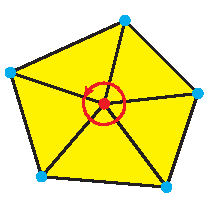
\includegraphics[width=\textwidth]{images/closed_fan}
			\caption{
				Manifold.
			}
			\label{fig:closed_fan}
		\end{subfigure}
		\begin{subfigure}[b]{0.3\textwidth}
			\centering
			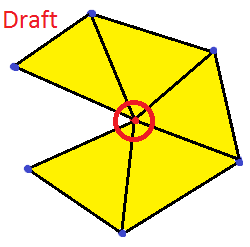
\includegraphics[width=\textwidth]{images/open_fan}
			\caption{
				Manifold.
			}
			\label{fig:open_fan}
		\end{subfigure}
		\\
		\begin{subfigure}[t]{0.32\textwidth}
			\centering
			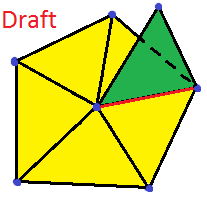
\includegraphics[width=\textwidth]{images/non_manifold_edge}
			\caption{
				Non-manifold.
			}
			\label{fig:non_manifold_edge}
		\end{subfigure}
		\begin{subfigure}[t]{0.32\textwidth}
			\centering
			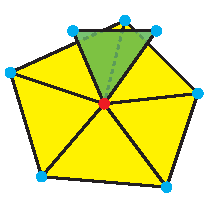
\includegraphics[width=\textwidth]{images/non_manifold_vertex}
			\caption{
				Non-manifold.
			}
			\label{fig:non_manifold_vertex}
		\end{subfigure}
		\begin{subfigure}[t]{0.32\textwidth}
			\centering
			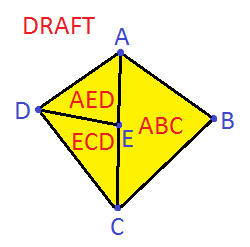
\includegraphics[width=\textwidth]{images/t_vertex}
			\caption{
				Non-manifold.
				}
			\label{fig:t_vertex}
		\end{subfigure}
		\caption{
			The upper images show a closed and opened fan of triangles incident to a vertex.
			Each edge is connected to only one or two faces.
			Both triangulations are 2-manifolds.
			%
			The bottom images show examples of not manifold meshes.
			The mesh in \subref{fig:non_manifold_edge} contains an edge with three incident triangles.
			The mesh in \subref{fig:non_manifold_vertex} contains a non-fan triangle connected to a vertex.
			A special case is the T-vertex problem shown in \subref{fig:t_vertex}:
			Vertex $E$ lies directly on edge $AC$.
			There is either a degenerate triangle $AEC$ with zero area, or triangle $ABC$ should be a quadrilateral with $E$ and should be split along $EB$.
		}
		\label{fig:manifold}
	\end{figure}


	\item[Orientable mesh] \hfill \\
	Concerning the orientation of meshes, a few terms are defined \cite{mesh_basics}:
	The orientation of a single face is the cyclic order of its vertices.
	This order is also called winding order and determines the direction of the surface normal.
	The orientation of two adjacent faces is said to be compatible, if the two shared vertices on the shared edge are in opposite order.
	A mesh is orientable if it is a manifold and any pair of adjacent faces are compatible.
	\Cref{fig:orientable_mesh} shows examples of orientable and not orientable meshes.

	\begin{figure}[H]
		\centering
		\begin{subfigure}[b]{0.3\textwidth}
			\centering
			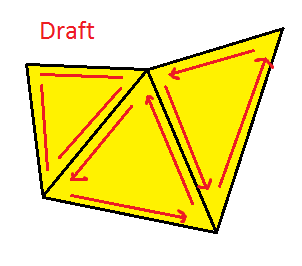
\includegraphics[width=0.8\textwidth]{images/orientable}
			\caption{Orientable mesh.}
			\label{fig:orientable}
		\end{subfigure}
		\begin{subfigure}[b]{0.3\textwidth}
			\centering
			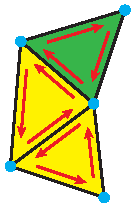
\includegraphics[width=0.8\textwidth]{images/not_orientable}
			\caption{Not orientable mesh.}
			\label{fig:not_orientable}
		\end{subfigure}
		\begin{subfigure}[b]{0.3\textwidth}
			\centering
			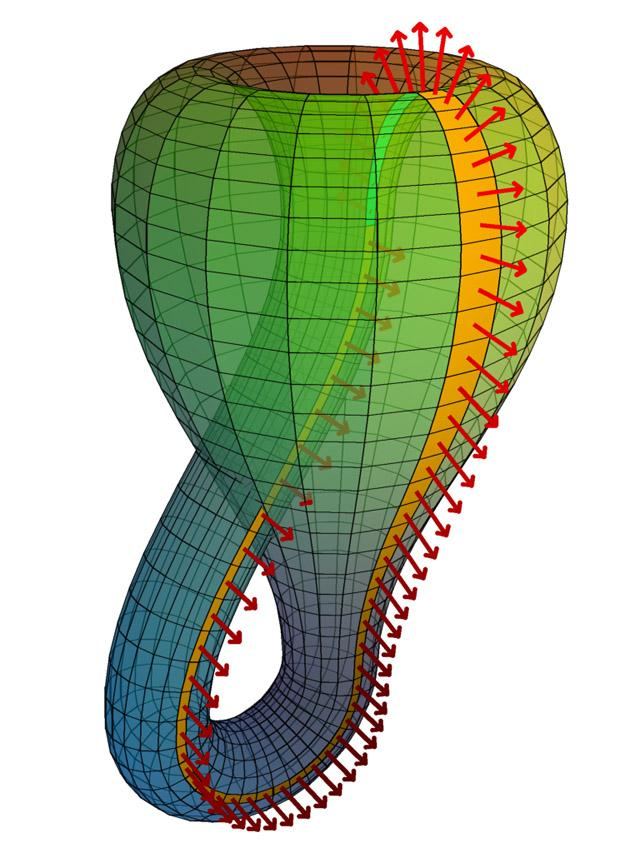
\includegraphics[width=\textwidth]{images/klein_bottle}
			\caption{The Klein bottle.}
			\label{fig:klein_bottle}
		\end{subfigure}
		\caption{
			The left and central image show an orientable and not orientable mesh.
			A mesh is orientable, if each pair of adjacent faces has a different vertex order on the shared edge.
			A famous example of a not orientable mesh is the Klein bottle on the right image, for which a strict inside and outside facing cannot be determined.
		}
		\label{fig:orientable_mesh}
	\end{figure}


	\item[Boundary] \hfill \\
	Edges of a mesh incident to only a face are called boundary edges.
	Vertices with an open fan of triangles are boundary vertices and connected to two boundary edges.
	A loop of connected boundary edges and vertices is called a boundary loop.


	\item[Closed/water-tight mesh] \hfill \\
	If a manifold mesh does not contain any boundary edges, which means that each vertex is part of a closed triangle fan, the mesh is a closed manifold.
	If a closed mesh is also orientable, it divides space into a half-space inside the mesh and one outside the mesh.
	The mesh is therefore a solid.
	The term water-tight is a common alias in CAM, meaning that a surface has no holes where water could enter or exit the solid represented by the mesh.


	%\item[Voronoi] \hfill \\


	\item[Delaunay triangulation] \hfill \\
	Named after the Russian mathematician Boris Delaunay, a 2-dimensional triangulation is called a Delaunay triangulation, when the circumcircle of each triangle does not contain a vertex of another triangle.
	The Delaunay triangulation is unique for each set of points, as long as not more than three vertices lie on a circle, \eg a square can be triangulated along any of the diagonals.
	The concept of 2-dimensional Delaunay triangulations can be extended to three dimensions, where each triangle of a manifold mesh has an empty circumscribing sphere.
	Such a triangle is sometimes also referred to as Gabriel 2-Simplex (G2S) \cite{g2s}.
	Delaunay triangulations produce very regular and visually appealing triangle meshes, as triangles with larger interior angles are preferred.
	\Cref{fig:delaunay_triangulation} shows a set of points with three different triangulations, with the first one being a Delaunay triangulation.

	\begin{figure}[H]
		\centering
		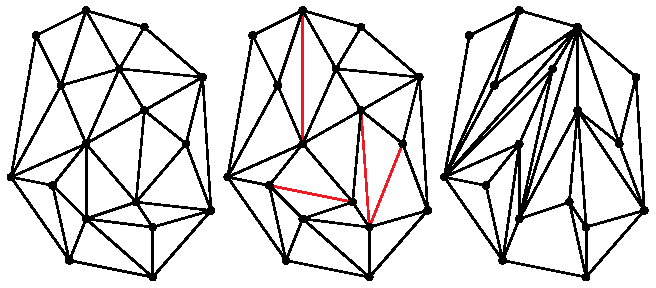
\includegraphics[width=0.9\textwidth]{images/delaunay_triangulation}
		\caption{
			Three different triangulations for the same set of points.
			Only the left one is a conforming Delaunay triangulation.
			The image in the middle is a constrained Delaunay triangulation with respect to the red constraints.
			Image adapted from \cite{delaunay_image}.
		}
		\label{fig:delaunay_triangulation}
	\end{figure}


	\item[Constrained Delaunay triangulation] \hfill \\
	Sometimes, predefined edges, \ie constraints or constrained edges, have to be respected when triangulating a point cloud into a Delaunay triangulation.
	The resulting triangulation is called a constrained Delaunay triangulation (CDT).
	Each triangle of the mesh satisfies the Delaunay condition, \ie an empty circumcircle, except for triangles containing a constrained edge.
	A CDT is therefore as close to a Delaunay triangulation as possible.
	\Cref{fig:delaunay_triangulation} shows a constrained Delaunay triangulation on the middle and the corresponding Delaunay triangulation on the left image.
	Constraints are colored red.
	By splitting the constrained edges using additional vertices, \ie Steiner points, a CDT can be further refined into a fully conforming constrained Delaunay triangulation.


	\item[Stock] \hfill \\
	The stock is the original piece of material which is used as input for a milling machine.
	Material is removed from the stock using cutters to shape the stock into a desired form.
	This process is called subtractive manufacturing.
	In virtual machining, the stock is a solid.


	\item[Swept volume] \hfill \\
	In the context of virtual machining, a single move of a cutting tool along a path is called a sweep.
	A swept volume is the volume which is covered by the cutting tool's solid during a sweep.
	The fast and efficient computation of such swept volumes for all kinds of paths, including self-intersection, is still subject to research and discussed in the field of envelope theory.


	\item[Feature] \hfill \\
	In CAD, a feature is a local peculiarity of a mesh.
	Features are typically geometrically interesting aspects of a mesh which are typical for the represented surface.
	A cube for example has sharp edges and a fork has tines.
	These properties identify an object and are vital to recognize it as such.
	In terms of surface reconstruction, features are typically aspects of the represented object which are hard to reconstruct and require extended processing.
	Examples would be sharp edges and corners, small holes or thin structures.

\end{description}

\section{Surface representations}
\label{sec:surface_representations}

CAD and CAM software uses several different representations for final and intermediate solids and geometric parts like cutters, the manufactured workpiece or the current machining state.
The following section is based on a comprehensive overview with sketches and descriptions of the most commonly used representations in the area of virtual machining \cite{virtual_machining_review}.

\begin{description}
	\item[Vector clipping] \hfill \\
	Vector clipping is mainly used in CAE to verify the correctness of a generated NC program before it is run on an actual milling machine.
	It was first described by Chappel \cite{vector_clipping} in 1983.
	The method requires the surface of the final workpiece as well as the stock.
	Initially, points on the final workpiece are calculated together with surface normals, \ie a point cloud, where the normals are not of unit length but long enough to reach the surface of the stock.
	To simulate the manufacturing process, the cutter is moved over this point cloud and the vectors attached to the points are clipped by the moving cutter, \cf \cref{fig:vector_clipping}.
	This method can be compared to a lawn mower, which cuts the grass, \ie the normal vectors, towards the ground, \ie the final workpiece.
	After cutting has completed, the lengths of the remaining vectors indicate the local error of the NC program.
	Vectors with positive lengths mark areas where too less material was removed and vice versa.
	The vector lengths are finally used to color the final workpiece where the color indicates the severity of the machining error.

	\begin{figure}[H]
		\centering
		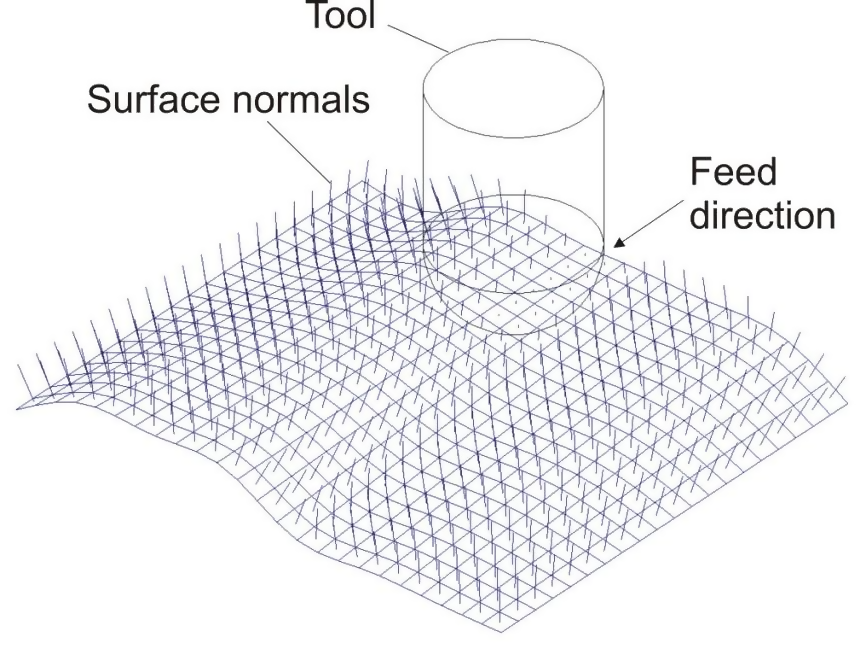
\includegraphics[width=0.5\textwidth]{images/vector_clipping}
		\caption{
			The vector clipping method \cite{virtual_machining_review}.
		}
		\label{fig:vector_clipping}
	\end{figure}


	\item[Z-maps and depth images] \hfill \\
	Describing solids using z-maps has been proposed by Anderson \cite{zmap} in 1978.
	It is furthermore the most widespread representation used in 3-axis material removal simulations.
	Z-maps approximate a solid by sampling its height at each crossing of a regular 2-dimensional grid.
	This grid is usually placed perpendicular to the cutting direction at one side of the stock, \eg the bottom.
	The volume of the z-mapped solid can be seen as the union of right square prisms where a prism is placed on each crossing of the grid with the height sampled at the crossing.
	\Cref{fig:zmap} shows such a prism approximation of a cuboid stock with a ball-end cutter removing material.
	As a z-map is a 2-dimensional scalar field with values at discrete regular positions, it can therefore be seen as an image, commonly referred to as depth image, \cf \cref{fig:depth_image}.

	Material is removed by creating a depth image for each cutter movement, \ie a sweep, with the same position and orientation as the depth image of the workpiece.
	The sweep's depth image describes the removed material during the sweep.
	It is combined with the depth image of the workpiece by updating all depth values to be the minimum value of the workpiece's and sweep's depth image.

	Processing depth images can be greatly accelerated using GPUs as they contain special hardware for dealing with per-pixel depth information, \ie depth buffer or z-buffer.

	However, z-map representations have a fundamental drawback.
	As each depth value can only store the distance to a single surface points, z-maps cannot represent solids with a back-face or covered surfaces.

	\begin{figure}[H]
		\centering
		\begin{subfigure}[b]{0.4\textwidth}
			\centering
			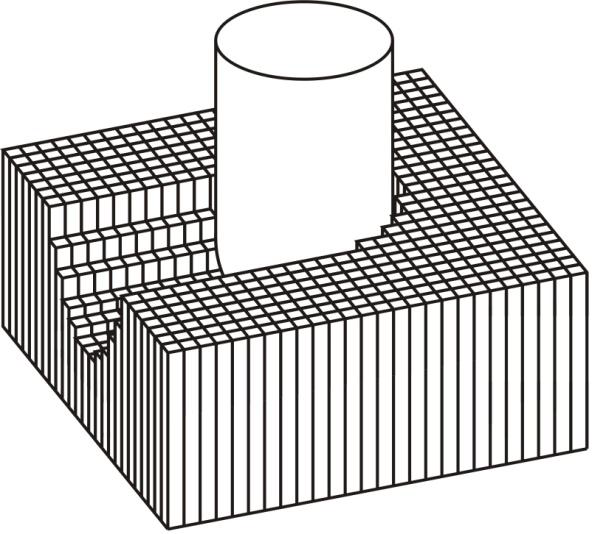
\includegraphics[width=\textwidth]{images/zmap}
			\caption{Z-map representation.}
			\label{fig:zmap}
		\end{subfigure}
		\begin{subfigure}[b]{0.4\textwidth}
			\centering
			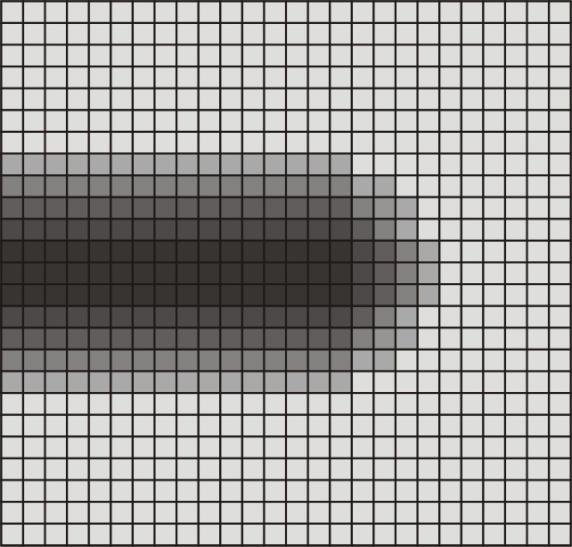
\includegraphics[width=\textwidth]{images/depth_image}
			\caption{Depth image.}
			\label{fig:depth_image}
		\end{subfigure}
		\caption{
			Representation of a cuboid stock with material removed using a ball-end cutter.
			The solid described by the z-map is represented using right square prisms in the left image.
			The z-map can be stored in a grayscale image as shown on the right  \cite{virtual_machining_review}.
		}
	\end{figure}


	\item[Dexel images] \hfill \\
	Dexel-based representations have been proposed by Hook to circumvent the shortcomings of depth images \cite{dexel}.
	Instead of a scalar value per pixel of a regular 2-dimensional grid, z-maps, a complex data element is stored, called a dexel, abbreviated from depth element.
	A dexel is created by tracing a ray, starting at a grid point, perpendicular to the grid's plane through the workpiece and collecting all surface intersections.
	Therefore, a 2-dimensional dexel image is sometimes also referred to as ray-rep, abbreviated from ray representation.
	Each dexel stores a sorted list of these intersections, where an intersection is also called a dexel node.
	A node basically contains the depth value of the intersection and can contain further information such as a surface normal or a color value.
	Pairs of dexel nodes where the first node has been an entry and the second an exit are called segments and always lie inside the workpiece.
	\Cref{fig:dexel_image} shows a dexel representation of a half sphere with a smaller, concentric half sphere drilled out.

	Material removal is done in a similar fashion as with z-maps.
	A dexel image is created for a sweep and then combined with the dexel image of the current workpiece.
	Instead of updating to the minimum value as done with z-maps, a 1-dimensional Boolean subtraction of all sweep dexels from the workpiece dexels is performed.

	In comparison with image-based representations like z-maps and depth images, dexel-based approaches are able to represent overlapping surfaces and workpieces with a front- and a back-face.
	Nevertheless, the sampling resolution from the surface's perspective is dependent on the orientation of the surface towards the dexel grid.
	The more parallel the surface lies to to the grid, the smaller becomes the distance between two neighboring entry/exit points on the surface.
	In case the surface is perpendicular to the grid, the dexels lie parallel to the surface and do not capture any intersections.

	\begin{figure}[H]
		\centering
		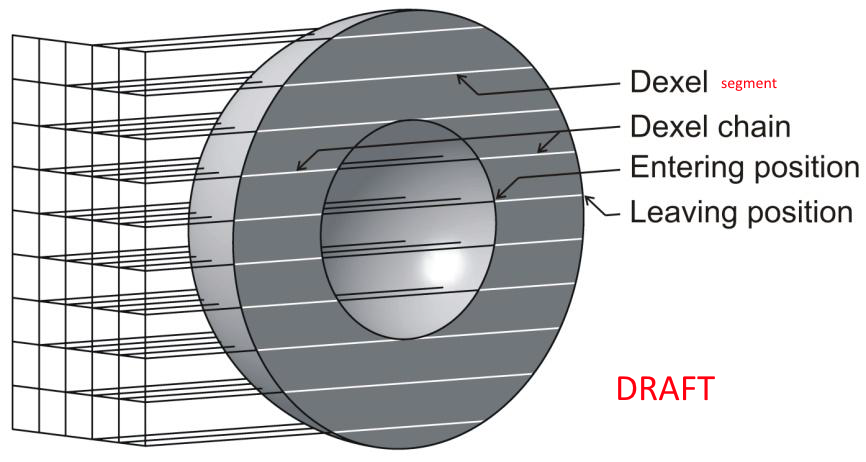
\includegraphics[width=0.8\textwidth]{images/dexels}
		\caption{
			Dexel image of a half sphere with a smaller, concentric half sphere drilled out \cite{virtual_machining_review}.
		}
		\label{fig:dexel_image}
	\end{figure}


	\item[Multi-dexel images] \hfill \\
	To increase the accuracy of dexel-based models, especially in regions of the surface where the surface normals are parallel to the dexels, multiple dexel images can be used.
	This idea was described by Benouamer \etal in 1997 to provide a good representation that can combine B-rep and CSG models \cite{tridexel_intersection}.
	Although multiple dexel images can be created from any orientations, it is common to create three dexel images along the three axes of a Cartesian coordinate system.
	Therefore, the 2-dimensional dexel grids lie in the three planes defined by pairs of the coordinate system's axes, \ie xy-, yz-, zx-plane.
	This case of multi-dexel image is also referred to as triple- or tri-dexel image.
	\Cref{fig:tri_dexel_image} shows a triple-dexel representation of an octant of a centered unit sphere.

	\begin{figure}[H]
		\centering
		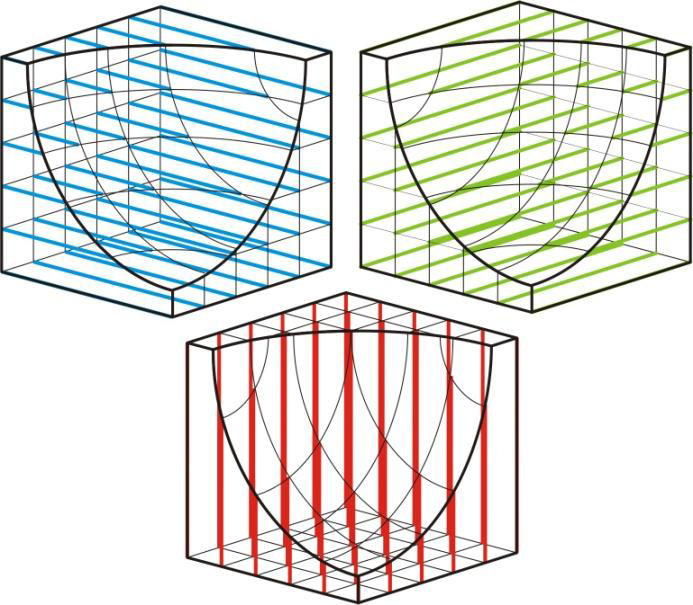
\includegraphics[width=0.8\textwidth]{images/tridexels}
		\caption{
			Tri-dexel images of an octant of a centered unit sphere.
			The left, blue image shows dexels along the x-axis, the centered, red image along the z-axis and the right, green image along the y-axis \cite{virtual_machining_review}.
		}
		\label{fig:tri_dexel_image}
	\end{figure}


	\item[Constructive Solid Geometry (CSG)] \hfill \\
	CSG is a technique widely spread in solid modeling.
	It has its origins in 1978 where Gossard \etal tried to use set theory to verify material removal in NC processes \cite{csg}.
	CSG describes a solid by its construction process from a set of simple primitives, making it therefore an interesting approach in procedural modeling.
	Although primitives are typically basic shapes such as cubes, spheres or cylinders, they can, in theory, be any kind of complex shape.
	Pairs of primitives can be combined using Boolean set operations such as union, intersection or difference.
	The result of such an operation is a new solid, which can be again combined with other models or further primitives.
	A good visualization of these combinations is as a tree as shown in \cref{fig:csg_tree}.

	In virtual machining, material removal can be described as iteratively subtracting a new solid corresponding to the swept volume of the cutter during a single movement.
	Additive manufacturing, e.g. 3-dimensional printing, is also easily representable by adding a new solid.

	CSG trees can also be rendered directly using OpenGL or DirectX by making use of the GPU's depth and stencil buffers.
	Well known algorithms in this area include Goldfeather's algorithm \cite{goldfeather} and Nigel's Sequenced Convex Subtraction (SCS) algorithm \cite{scs}.

	\begin{figure}[H]
		\centering
		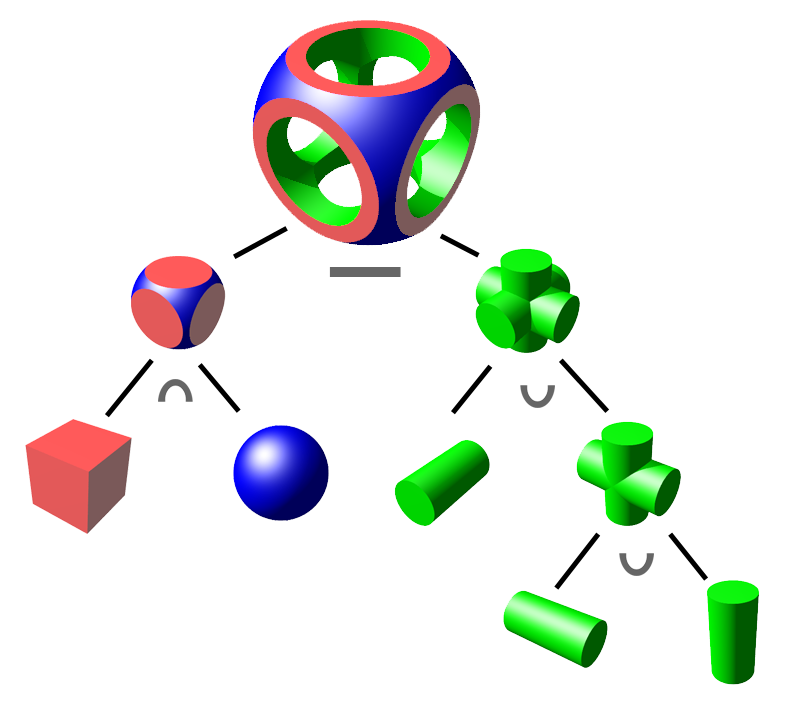
\includegraphics[width=0.8\textwidth]{images/csg_tree}
		\caption{
			A solid object modeled using CSG.
			The final shape of the object at the top is the result of combining the primitives at the bottom using Boolean operations \cite{csg_tree}.
		}
		\label{fig:csg_tree}
	\end{figure}

	\item[Spatial decomposition] \hfill \\
	The volume covered by a solid can also be represented by listing regions in 3-dimensional space which are occupied by the volume.
	This representation is also commonly known as spatial occupancy enumeration.
	To enumerate occupied regions, one must first decompose space into smaller regions.
	This can be done in a uniform or hierarchical manner.

	Uniform spatial decomposition (USD) divides space into equally sized cells.
	An example would be a regular grid with cubic cells.
	This special case is known as voxel model, where a voxel, abbreviated from volume element, is a single cell of the regular grid.
	\Cref{fig:spatial_decomposition_usd} shows a voxel model of a simple solid.

	USDs are simple to create and implement as they only require a three dimensional grid which stores for each cell whether it is occupied or not.
	Boolean operations are also easily solved, as two uniform grids can be combined on a per cell basis similar to z-maps.
	However, USDs are highly memory demanding to achieve a sufficient resolution to accurately represent a solid.
	Furthermore, a high resolution may only be needed in certain regions of the solid, \ie features.

	Hierarchical spatial decomposition (HSD) overcomes the shortcomings of USDs.
	HSDs partition space in an adaptive way and increase their resolution only where detail is necessary.
	Therefore, HSDs usually require less memory at the cost of increased complexity.
	\Cref{fig:spatial_decomposition_hsd} shows an example of a solid represented by a hierarchically decomposed space.

	A common representative of HSDs are octrees.
	An octree on its highest level is a cube which is then recursively subdivided into eight half-sized cubes, called octants.
	This subdivision is only done, where a finer decomposition of space is necessary.
	Further examples of hierarchical decompositions are Binary Space Partitioning (BSP) and Bounding Volume Hierarchies (BVH).

	\begin{figure}[H]
		\centering
		\begin{subfigure}[b]{0.2\textwidth}
			\centering
			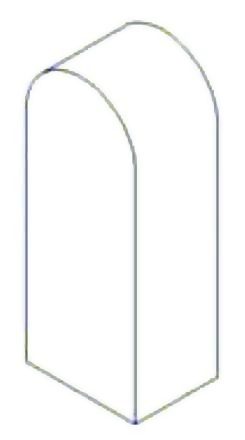
\includegraphics[width=\textwidth]{images/spatial_decomposition_solid}
			\caption{Solid}
			\label{fig:spatial_decomposition_solid}
		\end{subfigure}
		\begin{subfigure}[b]{0.2\textwidth}
			\centering
			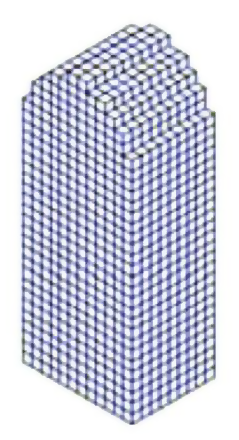
\includegraphics[width=\textwidth]{images/spatial_decomposition_usd}
			\caption{USD}
			\label{fig:spatial_decomposition_usd}
		\end{subfigure}
		\begin{subfigure}[b]{0.2\textwidth}
			\centering
			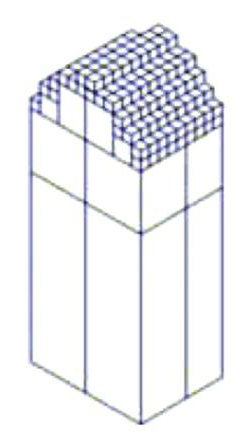
\includegraphics[width=\textwidth]{images/spatial_decomposition_hsd}
			\caption{HSD}
			\label{fig:spatial_decomposition_hsd}
		\end{subfigure}
		\caption{
			The solid on the left side can be described using spatial decomposition in either a uniform manner, central image, or a hierarchical manner, right image \cite{virtual_machining_review}.
		}
		\label{fig:spatial_decomposition}
	\end{figure}


	\item[Boundary representation (B-rep)] \hfill \\
	Boundary representations, are the most wide-spread representations used in modern CAD systems.
	As the term suggests, B-reps describe a solid by specifying its boundary surface.
	This surface typically consists of faces, \ie bounded surfaces, edges between those faces, \ie bounded curves, vertices, \ie 3-dimensional points, as well as their topology.
	B-reps are therefore closed meshes.
	Faces can be specified using a variety of mathematical models from complex splines such as B-splines and NURBs to simple polygons like triangles.
	\Cref{fig:brep} shows an example of a B-rep which represents a machining part using triangles as faces.
	%
	In the field of virtual machining, the faces of B-reps are typically polygons which are connected by straight edges, \ie polyhedrons.
	The most common case are triangle meshes, although quadrilateral meshes are also popular in CAD.
	%
	Boolean operations like subtraction are hard to perform on arbitrary B-reps.
	When considering only triangulated surfaces, boolean operations become manageable, but still remain calculatively expensive and usually suffer from numeric instabilities.
	Boolean operations on triangulated B-reps are typically available in modern CAD kernels.

	\begin{figure}[H]
		\centering
		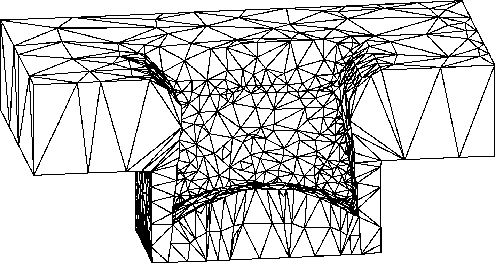
\includegraphics[width=0.8\textwidth]{images/brep}
		\caption{
			A boundary representation describes a machining part be specifying its boundary surface. A popular surface representation is a set of connected triangles \cite{virtual_machining_review}.
		}
		\label{fig:brep}
	\end{figure}

	\item[Functional representation (F-rep)] \hfill \\
	From a more mathematical point of view, surfaces can also be represented using real-valued functions.
	Pasko \etal give a good overview on this subject in the context of modeling and computer graphics \cite{frep}.
	A sphere, for example, is defined analytically as the infinite set of points with the same distance, \ie radius, to a distinct center point $c$.
	By defining a function $d$ for the distance of a point $p$ to the center $c$,
	\begin{align}
		d(p) &= \lvert c - p \rvert,
		\intertext{a sphere $S$ with radius $r$ is defined as a set of points}
		S &= \{\, p \in \mathbb{R}^3 \mid d(p) - r = 0 \,\}.
	\end{align}
	Formally, $S$ is called a locus with regard to the condition $d(p) - r = 0$.
	
	Generalized, an object can be specified by classifying all spatial points using a continuous, real-valued function $f$.
	For each point $p \in \mathbb{R}^3$
	\begin{align}
		f(p) &> 0 \quad \text{if $p$ is inside the object,}               \notag \\
		f(p) &= 0 \quad \text{if $p$ is on the surface of the object and} \notag \\
		f(p) &< 0 \quad \text{if $p$ is outside the object.}              \notag
	\end{align}

	Functional representations excel in exactness, expressiveness and memory requirements.
	Additionally, some classes of problems are easier to solve on analytical models, \eg intersection tests.
	Furthermore, Boolean operations and manipulations like bending and twisting are easier to formulate on mathematical entities then on the other data structures discussed in this section, \cf Boolean operations on signed distance functions \cite{extended_marching_cubes}.

	Many primitives used in CSG are typically described using F-reps.
	Several CAD kernels also use F-reps internally to retain precision until the final result is exported, where it is typically tessellated into a B-rep.

\end{description}

\chapter{Previous work}
\label{ch:previous_work}

As mentioned in the problem statement in \cref{sec:problem} the focus of the implementations underlying this thesis is to develop multiple strategies to extract a triangulated surface mesh from the data model used inside the VML.
To ease the understanding of the implementations presented in this thesis, a short introduction to the VML and its data model is given.
Parts of this description have been taken from the author's bachelor thesis, where the data model has been previously described with a focus on visualization \cite{bachelor}.

\section{Project history}
\label{sec:project_history}

% TODO: rethink choice of past vs. present tense
From the middle of 2011 to the end of 2013 the project Enlight was conducted for research by the RISC Software GmbH in Hagenberg im Mühlkreis, Austria.
Enlight's goals were the development of a faster, scalable and numerically stable method for modeling and visualizing subtractive manufacturing.
Enlight uses a regular grid data structure to store a stock solid and add precomputed swept volumes.
A triangle elimination strategy is employed to keep the total number of triangles held by the grid within manageable bounds, \cf classification in \cref{sec:classification}.
For visualization, a custom raycasting approach was developed \cite{enlight} and accelerated using GPUs and many-core architectures.

From the beginning to the end of 2014, the follow-up research project Engrave focused on solving swept volume computation for arbitrary cutter geometries and tool paths.
Engrave basically allows dynamic swept volume computation from a set of cutter solids and transformation lists.
Swept volume computation is done by extruding a point cloud along the tool path and then reconstructing a closed triangle mesh from it using a parallel and highly optimized variant of the ball pivoting algorithm \cite{engrave}.
The computed swept volumes where directly imported into Enlight's data model.

With the beginning of 2015, the prototype developed during Enlight and Engrave was rebranded to Virtual Machining Library (VML) and, later that year, to Virtual Modeling Library.
The VML is currently further developed as a commercial product.
\Cref{fig:vml_demo} shows a small demonstration of the VML.

\begin{figure}[h]
	\centering
		\begin{subfigure}[t]{0.32\textwidth}
			\centering
			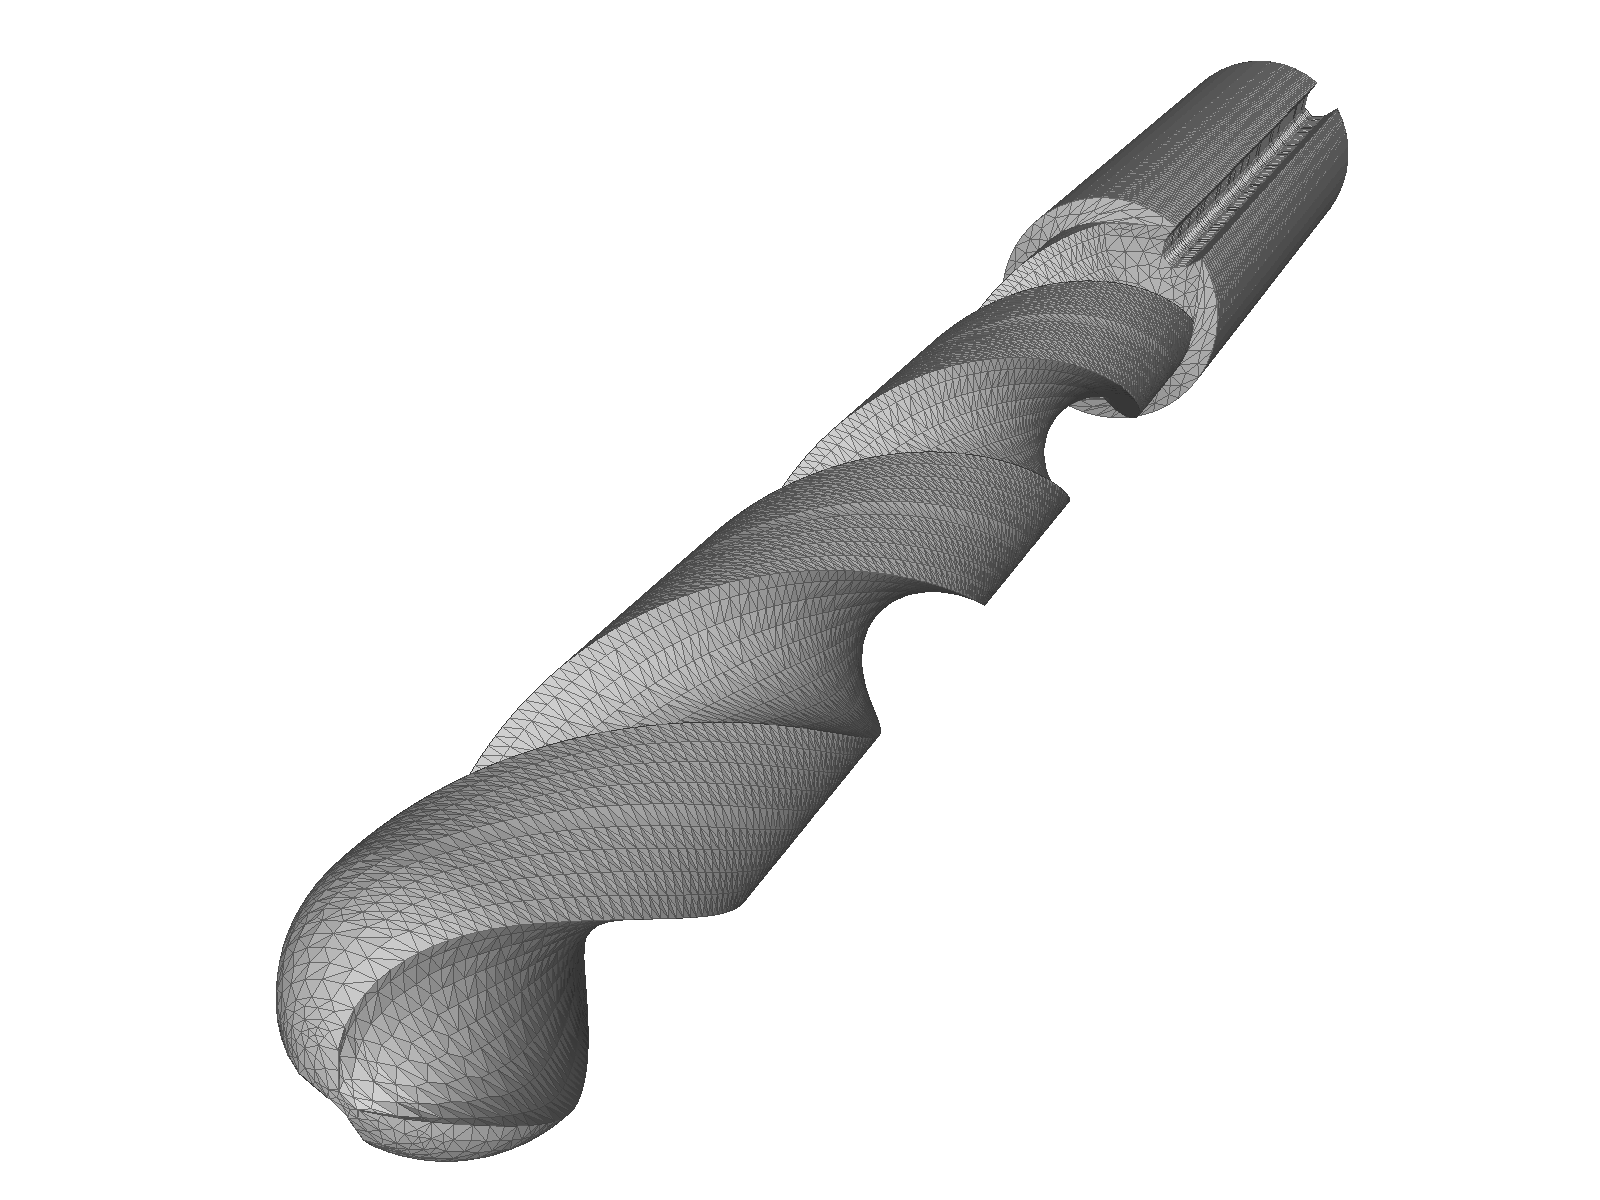
\includegraphics[width=\textwidth]{images/hq_impeller_tool}
			\caption{Ball-end cutter.}
			\label{fig:hq_impeller_tool}
		\end{subfigure}
		\begin{subfigure}[t]{0.32\textwidth}
			\centering
			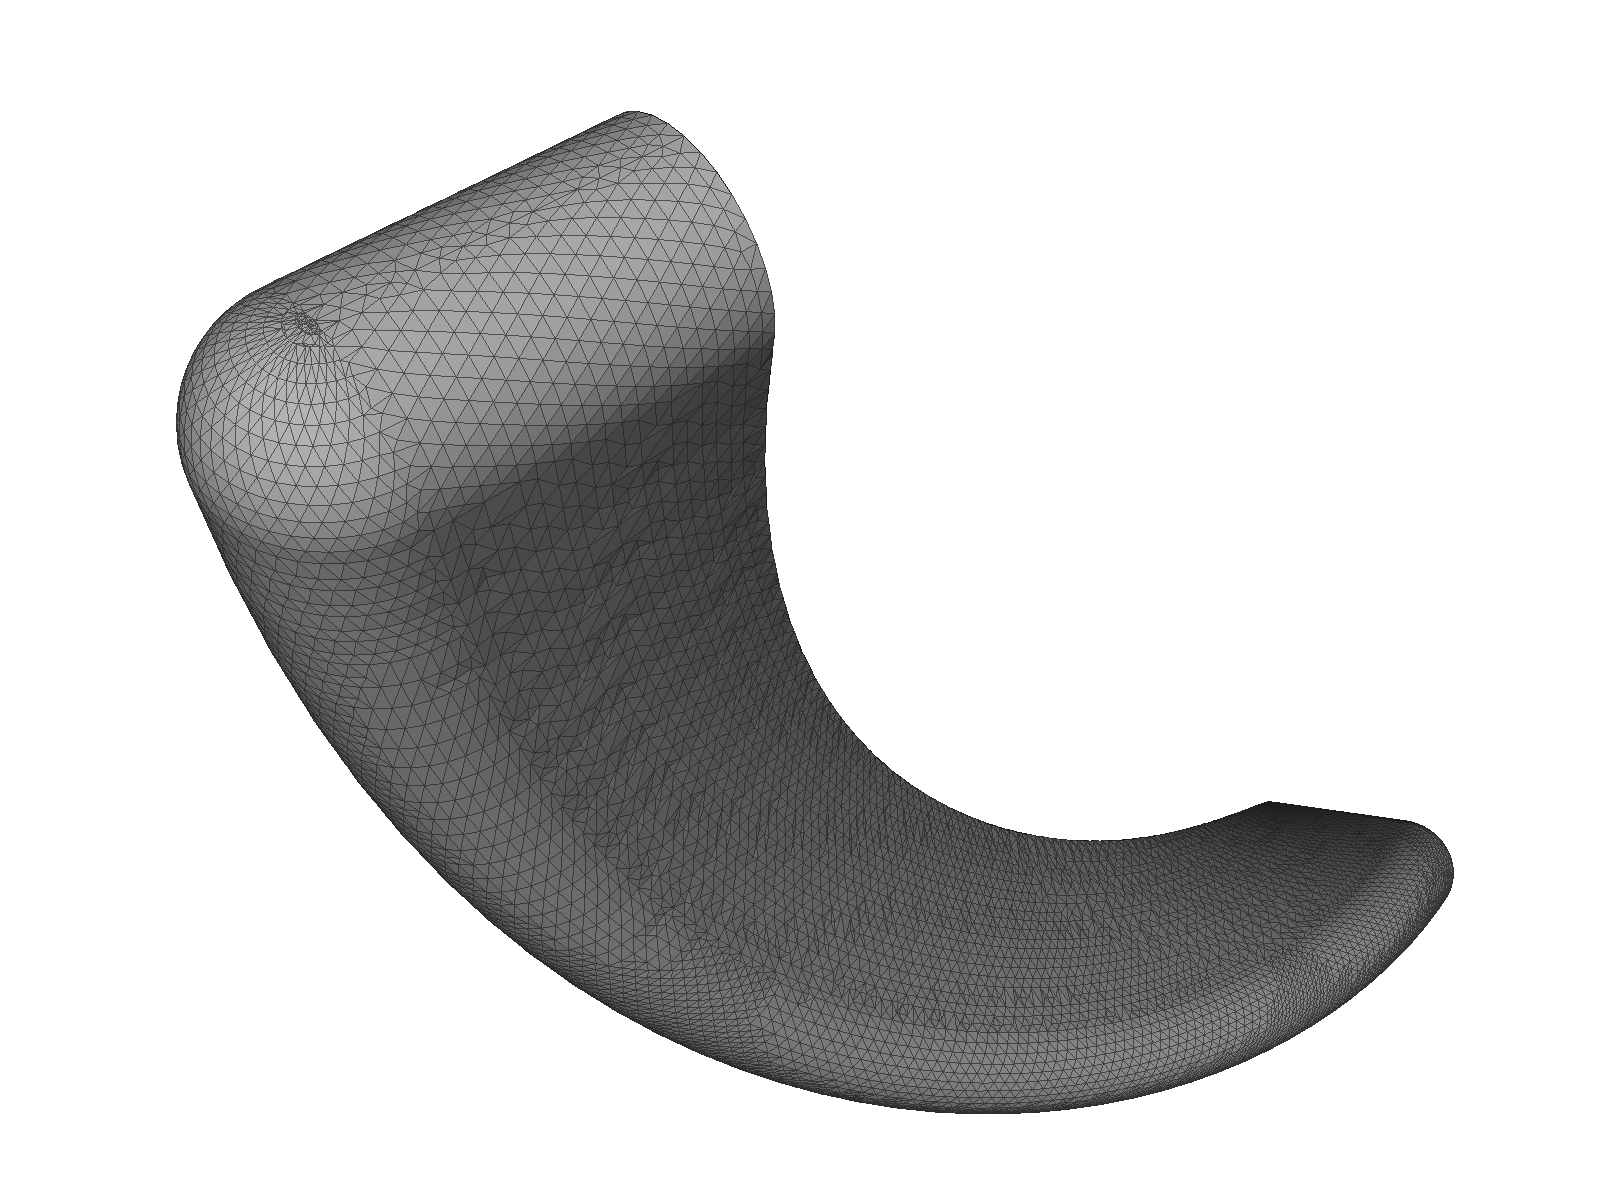
\includegraphics[width=\textwidth]{images/hq_impeller_swept}
			\caption{Swept volume.}
			\label{fig:hq_impeller_swept}
		\end{subfigure}
		\begin{subfigure}[t]{0.32\textwidth}
			\centering
			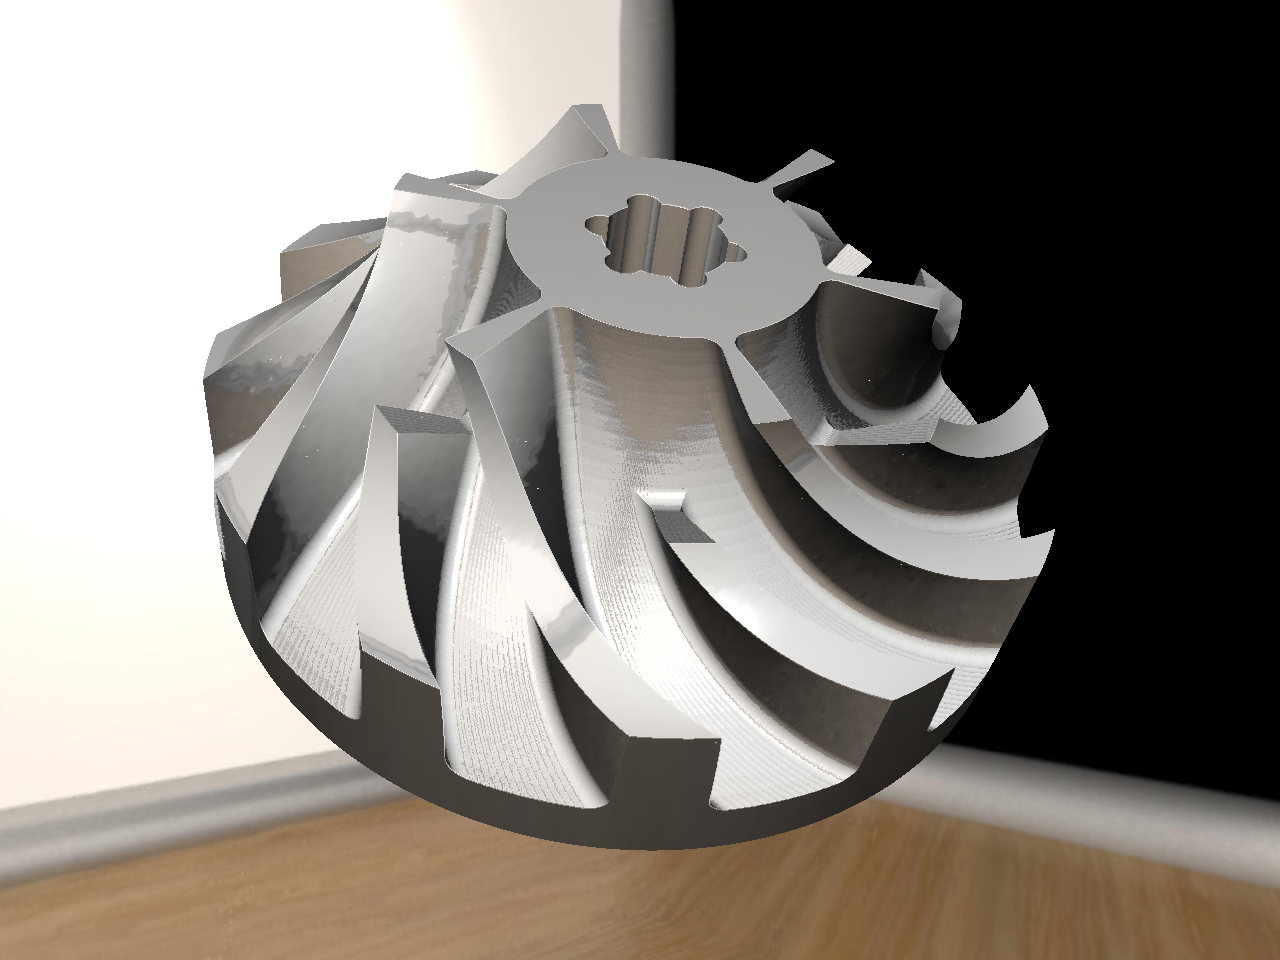
\includegraphics[width=\textwidth]{images/hq_impeller_complete}
			\caption{Machined impeller.}
			\label{fig:hq_impeller_complete}
		\end{subfigure}
		\\
		\begin{subfigure}[t]{0.32\textwidth}
			\centering
			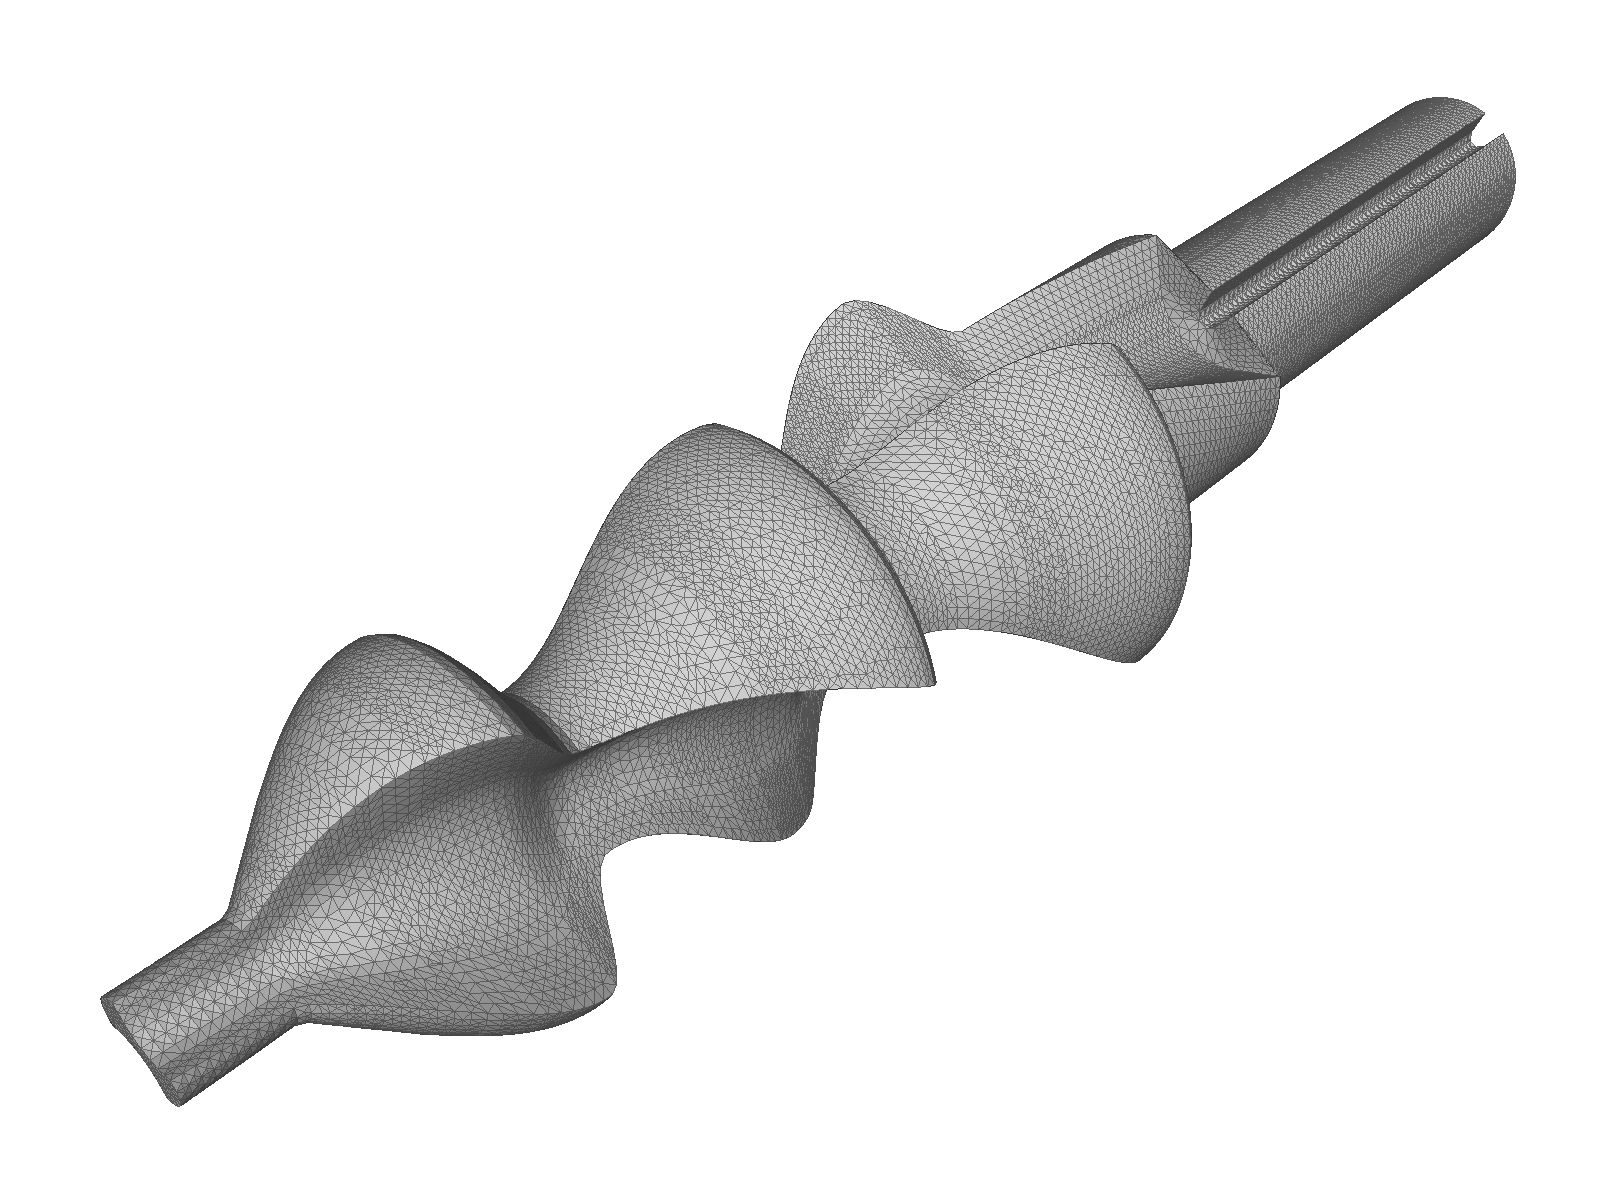
\includegraphics[width=\textwidth]{images/turbine_tool}
			\caption{Fir tree cutter.}
			\label{fig:turbine_tool}
		\end{subfigure}
		\begin{subfigure}[t]{0.32\textwidth}
			\centering
			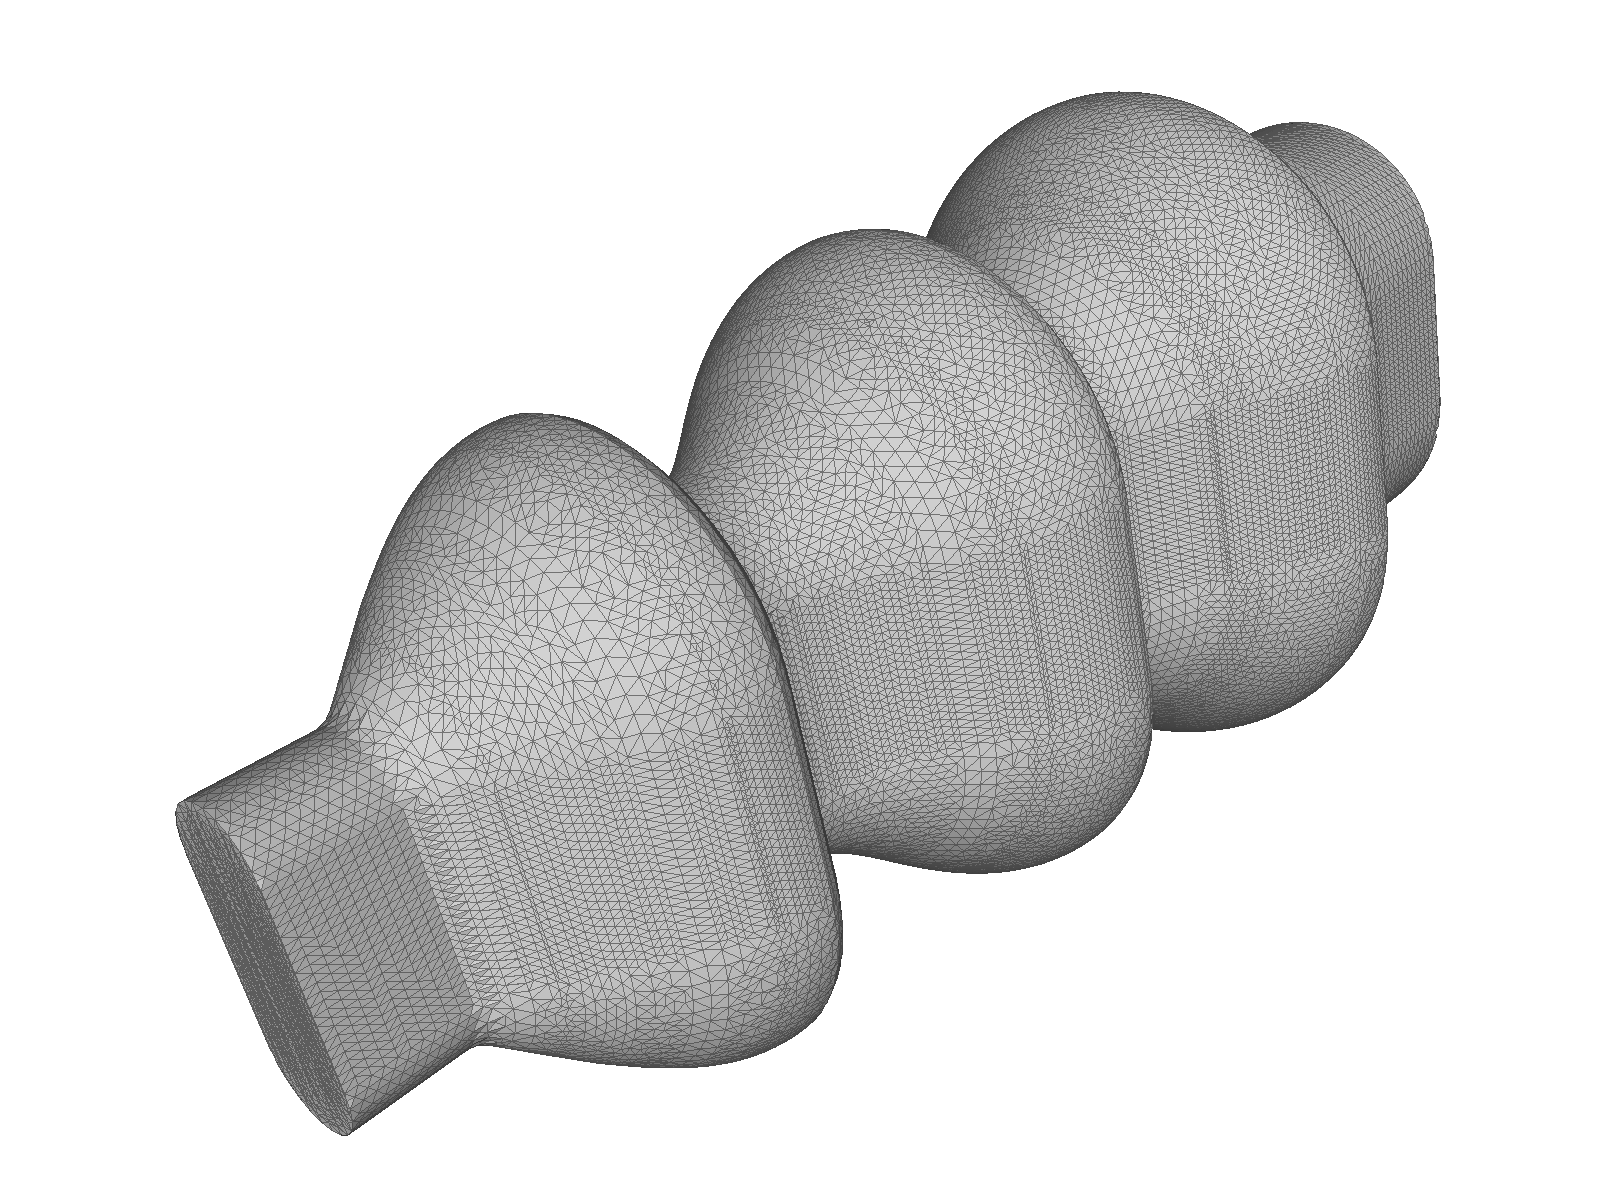
\includegraphics[width=\textwidth]{images/turbine_swept}
			\caption{Swept volume.}
			\label{fig:turbine_swept}
		\end{subfigure}
		\begin{subfigure}[t]{0.32\textwidth}
			\centering
			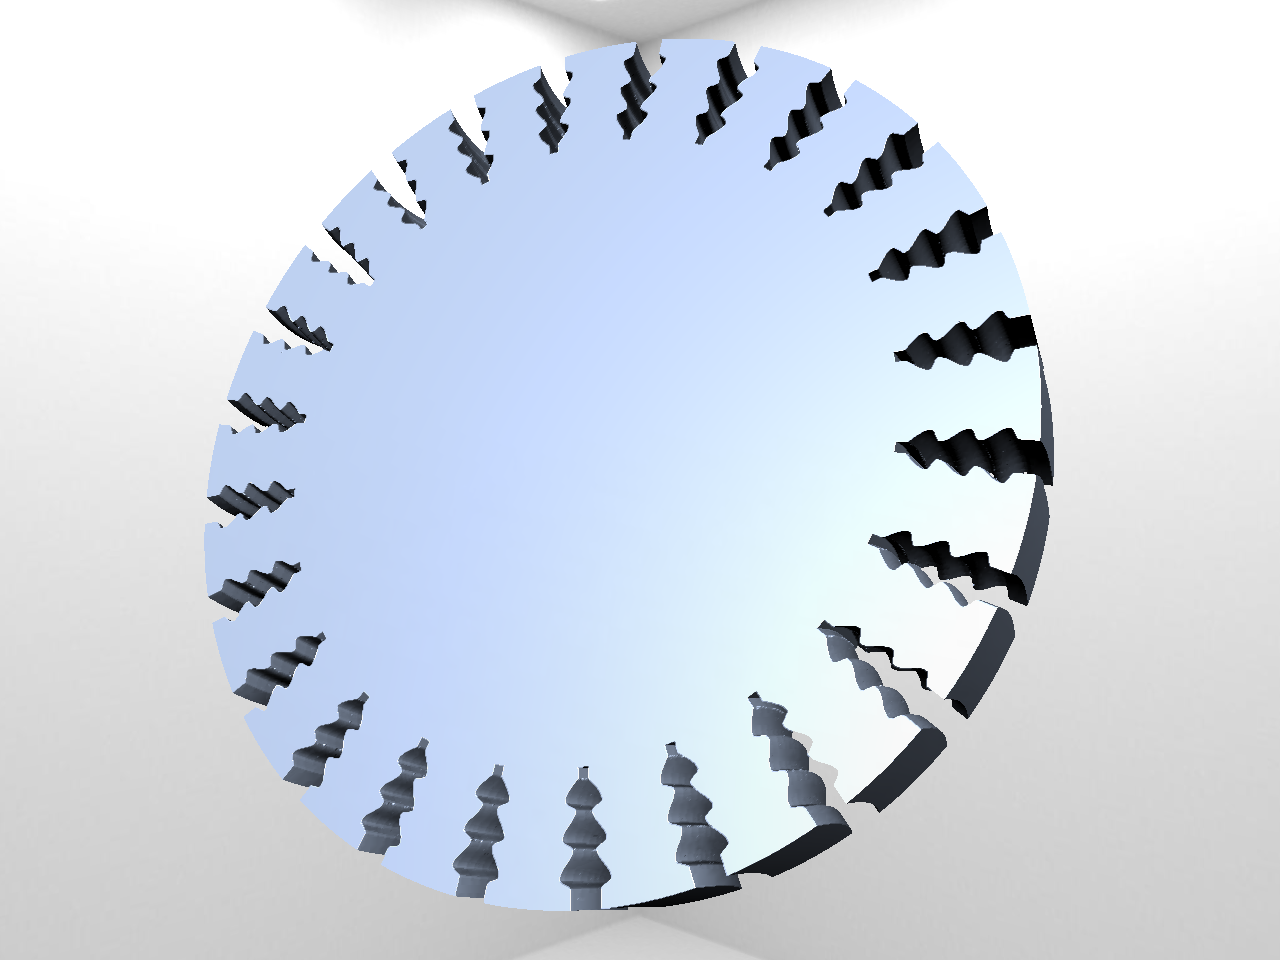
\includegraphics[width=\textwidth]{images/turbine_complete}
			\caption{Machined turbine wheel.}
			\label{fig:turbine_complete}
		\end{subfigure}
	\caption[VML demo]{
		Demonstration of the VML's capabilities.
		Cutter meshes, \cf \subref{fig:hq_impeller_tool} and~\subref{fig:turbine_tool}, are loaded and then transformed using a list of transformation matrices to calculate swept volumes, \cf \subref{fig:hq_impeller_swept} and~\subref{fig:turbine_swept}.
		By applying a series of these swept volumes to a stock, the machining of a workpiece is simulated.
		The result can be visualized using raycasting, \cf \subref{fig:hq_impeller_complete} and~\subref{fig:turbine_complete} \cite{engrave_report}.
	}
	\label{fig:vml_demo}
\end{figure}


\section{VML data model}
\label{sec:vml_data_model}

The primary purpose of the VML is to model, simulate and visualize subtractive manufacturing.
A typical workflow consists of loading a stock solid and then repeatedly sweeping various cutting tools over the stock.
These cutting tools are solid triangle meshes, loaded from disk, which are moved along paths, \ie lists of transformation matrices, to create swept volumes, \ie triangle meshes.
These swept volumes are then conceptually subtracted from the stock.
In fact, swept volumes are stored side by side together with the stock and theoretically build up a specialized CSG tree as shown in \cref{fig:vml_csg}.
A separate processing step is required to calculate the exact surface.
For visualization, the data model is sampled using a raycast which calculates a point on the surface for each ray, \cf \cref{sec:raycasting}.

\begin{figure}[h]
	\centering
	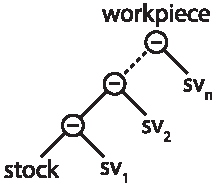
\includegraphics[width=0.5\textwidth]{images/vml_csg}
	\caption[VML CSG representation]{
		The input model held by the VML is similar to a linearized CSG tree.
		The initial stock solid is combined with a series of swept volumes using Boolean subtraction.
		The VML stores parts of the geometries of all leaves of this tree, \cf classification in \cref{sec:classification}.
	}
	\label{fig:vml_csg}
\end{figure}


The central data structure inside the VML, which holds the current state of the simulation, \ie the workpiece, is a regular 3-dimensional grid.
This data structure was originally chosen because it was directly used as acceleration structure for the raycasting subsystem.
Although there is a wide variety of acceleration structures available, \eg kd-trees, octrees, binary space partitioning (BSP) or bounding volume hierarchies (BVH), regular grids offer greater simplicity in organization and construction than the others.
This is especially beneficial in cases where those data structures have to be updated regularly.
Particularly animated scenes in computer-animated films or changing geometries as in virtual machining require frequent rebuilds or updates of those data structures.
Due to their simplicity and regularity, regular grids provide viable candidates for these scenarios.
However, the VML's regular grid is also the basis for a triangle count optimization called classification which is described in the following section.


\subsection{Classification}
\label{sec:classification}

Every time a solid triangle mesh, stock or swept volume, is added to the grid, the triangles of the mesh have to be mapped to the cells of the grid.
Thereby, each triangle is added to each cell it intersects.
A triangle is therefore potentially referenced from multiple cells.
When the mapping is complete, the affected cells are classified into one of three categories with respect to the newly added mesh.
Cells which are occupied by triangles of the mesh's surface are surface cells.
Cells inside and outside the mesh are inside and outside cells and contain no triangles.
The sketches in \cref{fig:classification_before,fig:classification_sv} illustrate the classification of a single solid inside the grid, \ie stock, as well as a swept volume before it is merged.

\begin{figure}[!h]
	\centering
	\begin{tabular}{cc}
		\begin{subfigure}[t]{0.3\textwidth}
			\centering
			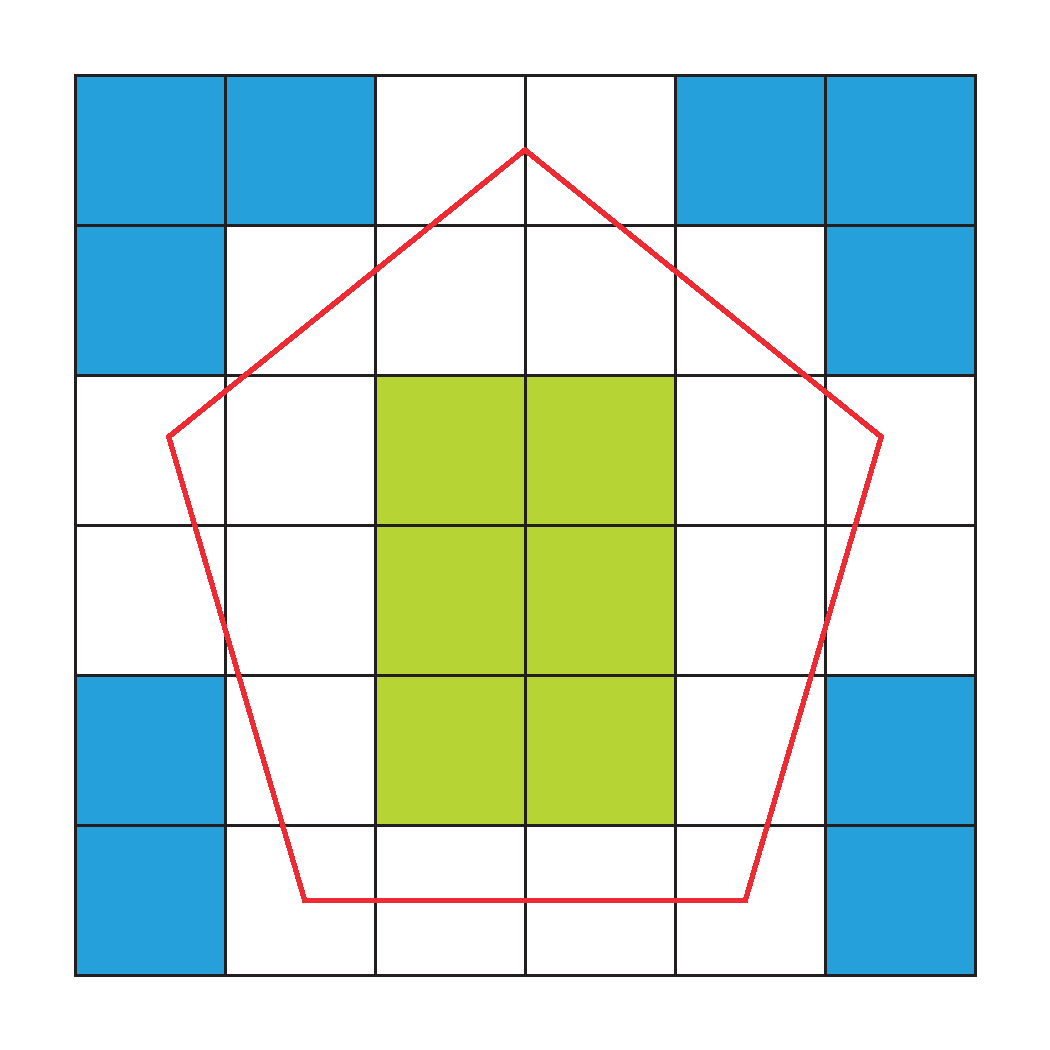
\includegraphics[width=\textwidth]{images/classification_before}
			\caption{Stock}
			\label{fig:classification_before}
		\end{subfigure}&
		\begin{subfigure}[t]{0.3\textwidth}
			\centering
			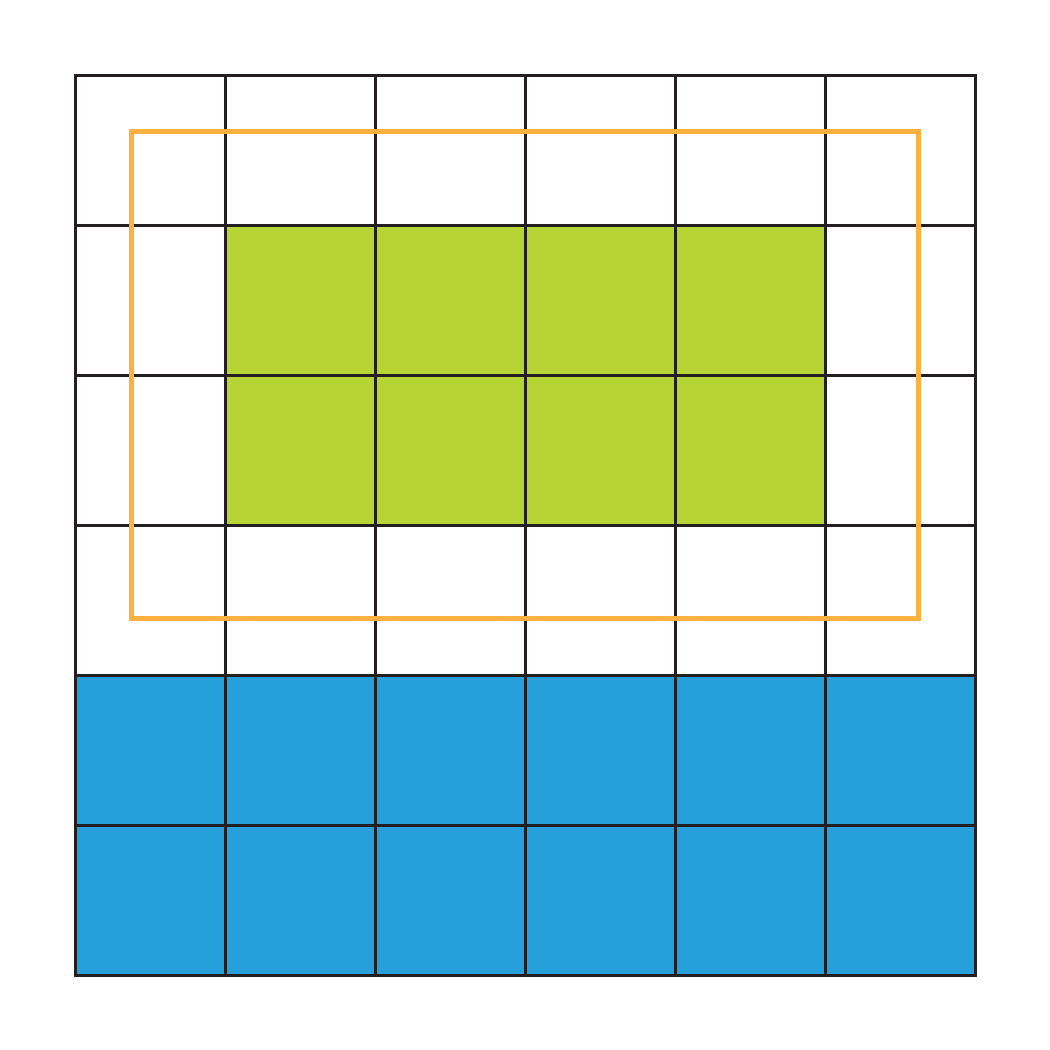
\includegraphics[width=\textwidth]{images/classification_sv}
			\caption{Swept volume}
			\label{fig:classification_sv}
		\end{subfigure}\\
		\begin{subfigure}[t]{0.3\textwidth}
			\centering
			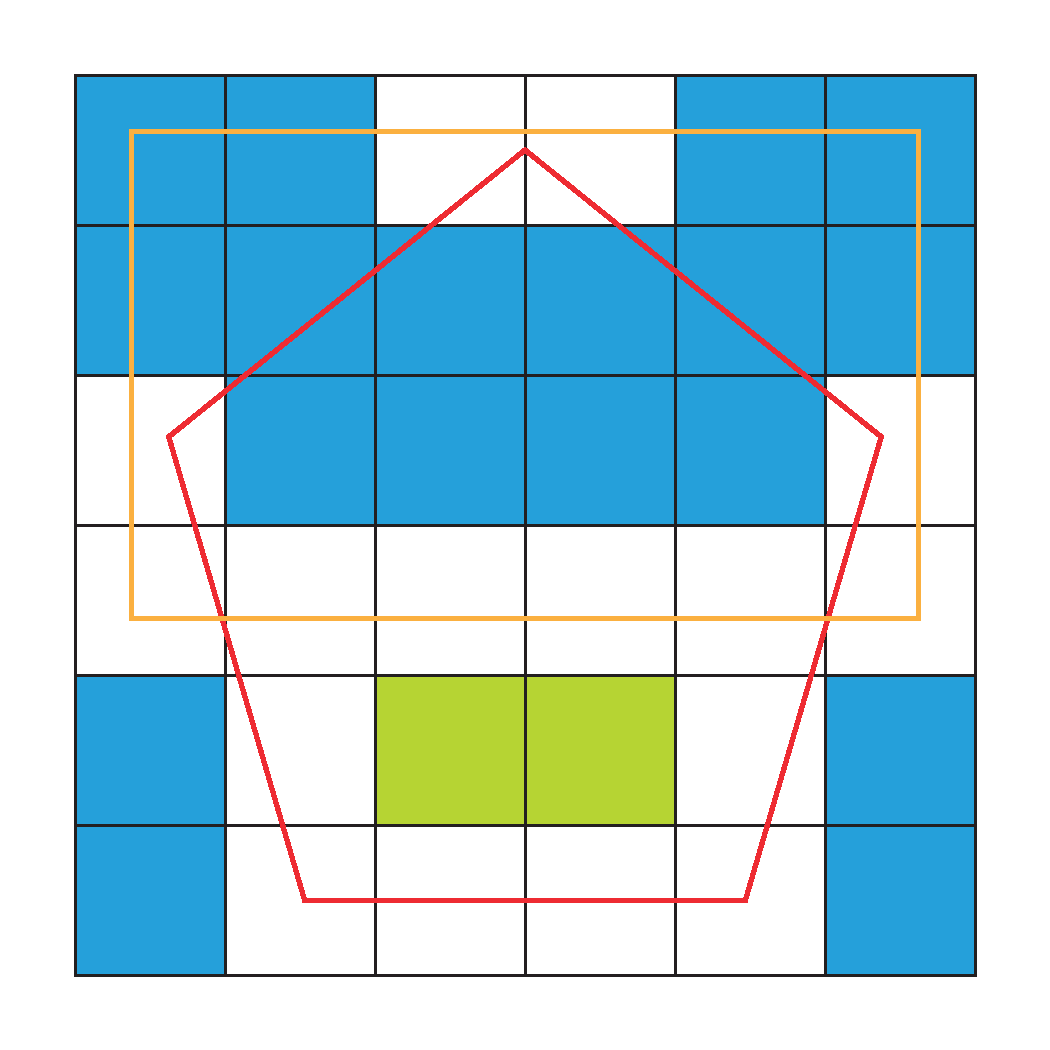
\includegraphics[width=\textwidth]{images/classification_after}
			\caption{Stock and swept volume}
			\label{fig:classification_after}
		\end{subfigure}&
		\begin{subfigure}[t]{0.3\textwidth}
			\centering
			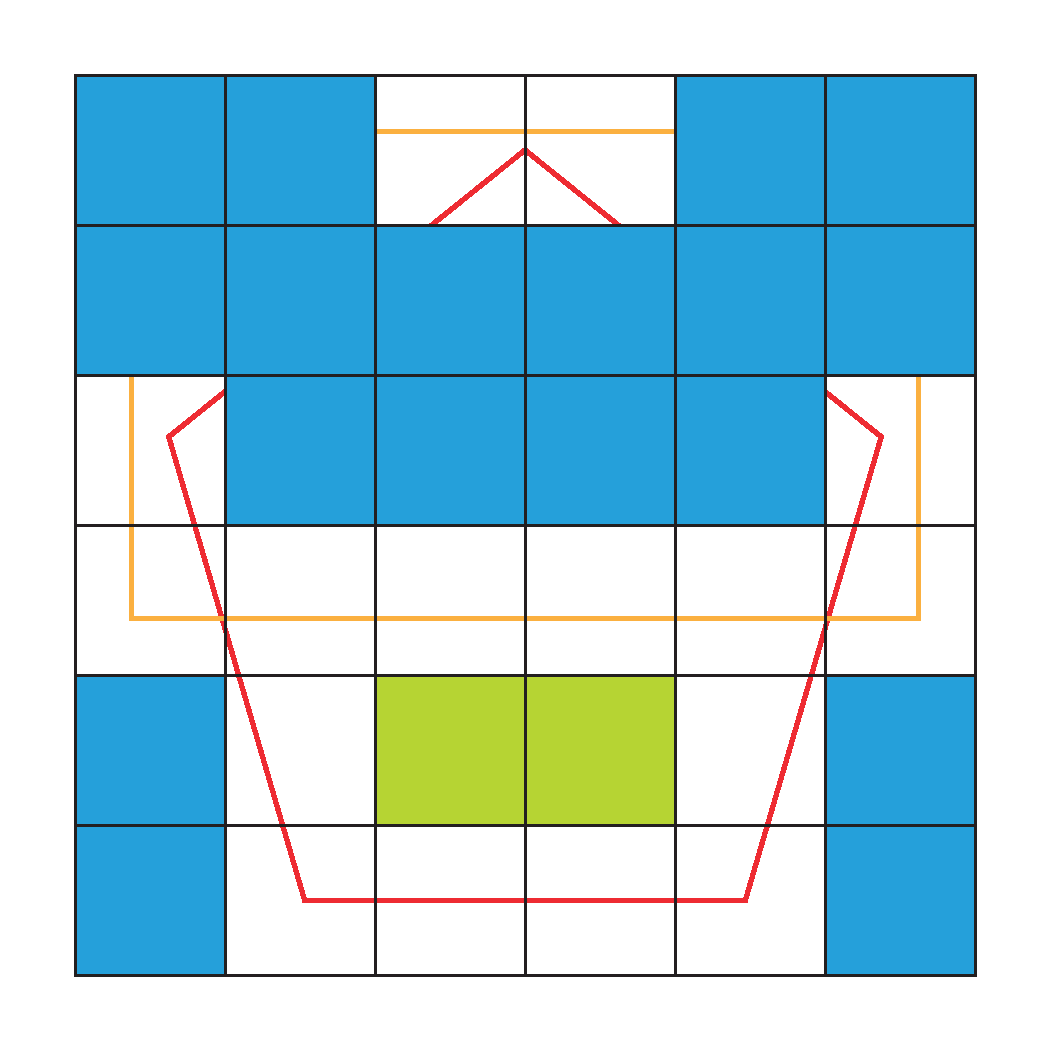
\includegraphics[width=\textwidth]{images/classification_after_removal}
			\caption{Triangle elimination}
			\label{fig:classification_after_removal}
		\end{subfigure}\\
	\end{tabular}
	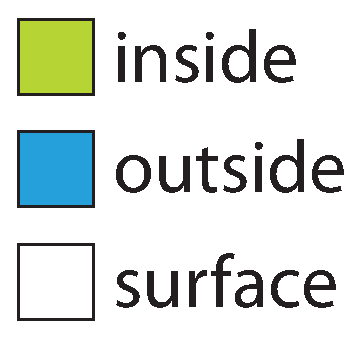
\includegraphics[width=0.1\textwidth]{images/classification_legend}
	\caption[Cell classification]{
		Principle of classifying cells according to the added mesh.
		The classification of the regular grid with a stock mesh, before a swept volume has been added, is shown in \subref{fig:classification_before}.
		The classification of the regular grid with regard to a new swept volume is shown in \subref{fig:classification_sv}.
		When the swept volume is added, both classifications are combined as shown in \subref{fig:classification_after}.
		Finally, triangles in outside cells can be removed as shown in \subref{fig:classification_after_removal}, cutting down the total number of stored triangles.
		For raycasting, only surface cells are relevant.
	}
	\label{fig:classification}
\end{figure}

When a new swept volume is added to the grid, its triangle mesh is classified itself and merged into the existing cell classification of the grid.
By limiting the modifiability of the scene to only allow subtracting swept volumes, a set of rules for merging a new mesh's classification into the grid's one can be derived and is shown in \cref{tbl:classification_rules}.

\begin{table}[h]
	\centering
	\begin{tabular}{p{2cm}p{2cm}|p{2cm}p{2cm}p{2cm}}
		                                                                &         & \multicolumn{3}{l}{Swept volume classification} \\
		                                                                &         & outside & surface & inside                      \\
		\midrule                                                                                                                    
		\multirow{3}{*}{\parbox{2cm}{Grid \\ classification \\ before}} & outside & outside & outside & outside                     \\
		                                                                & surface & surface & surface & outside                     \\
		                                                                & inside  & inside  & surface & outside                     
	\end{tabular}
	\caption{
		Classification rules when a new swept volume is added to the grid.
		On the left is the classification of a grid cell before the new volume has been added.
		On the top is the classification of a grid cell with regard to the new volume.
		The center of the table shows the outcome when these two classifications are merged.
	}
	\label{tbl:classification_rules}
\end{table}

When a new swept volume has been classified, it is merged into the grid's classification as follows:
Grid cells which are outside the added swept volume remain unchanged.
Surface cells of the added volume become surface cells except they were outside cells before.
Cells inside a swept volume always become outside cells, as they are \enquote{cut away} by the swept volume.
The result of merging a swept volume into the grid is visualized in \cref{fig:classification_after}.
After classification is complete, all triangles in outside cells can be removed, \cf \cref{fig:classification_after_removal}.

This strategy allows to keep the total number of triangles under control as the system should be able to support a large number of swept volumes, theoretically infinite if triangles are regularly eliminated.
%
However, this kind of reduction has a significant consequence.
As the contents of outside cells are simply deleted, the stored geometries are no longer closed meshes.
\Cref{fig:cylinders_classification} shows the effects of triangle elimination by example.
Surface points can still be calculated as shown by the example of the raycast used for visualization in \cref{sec:raycasting}.

\begin{figure}[!h]
	\centering
	\begin{subfigure}[b]{0.4\textwidth}
		\centering
		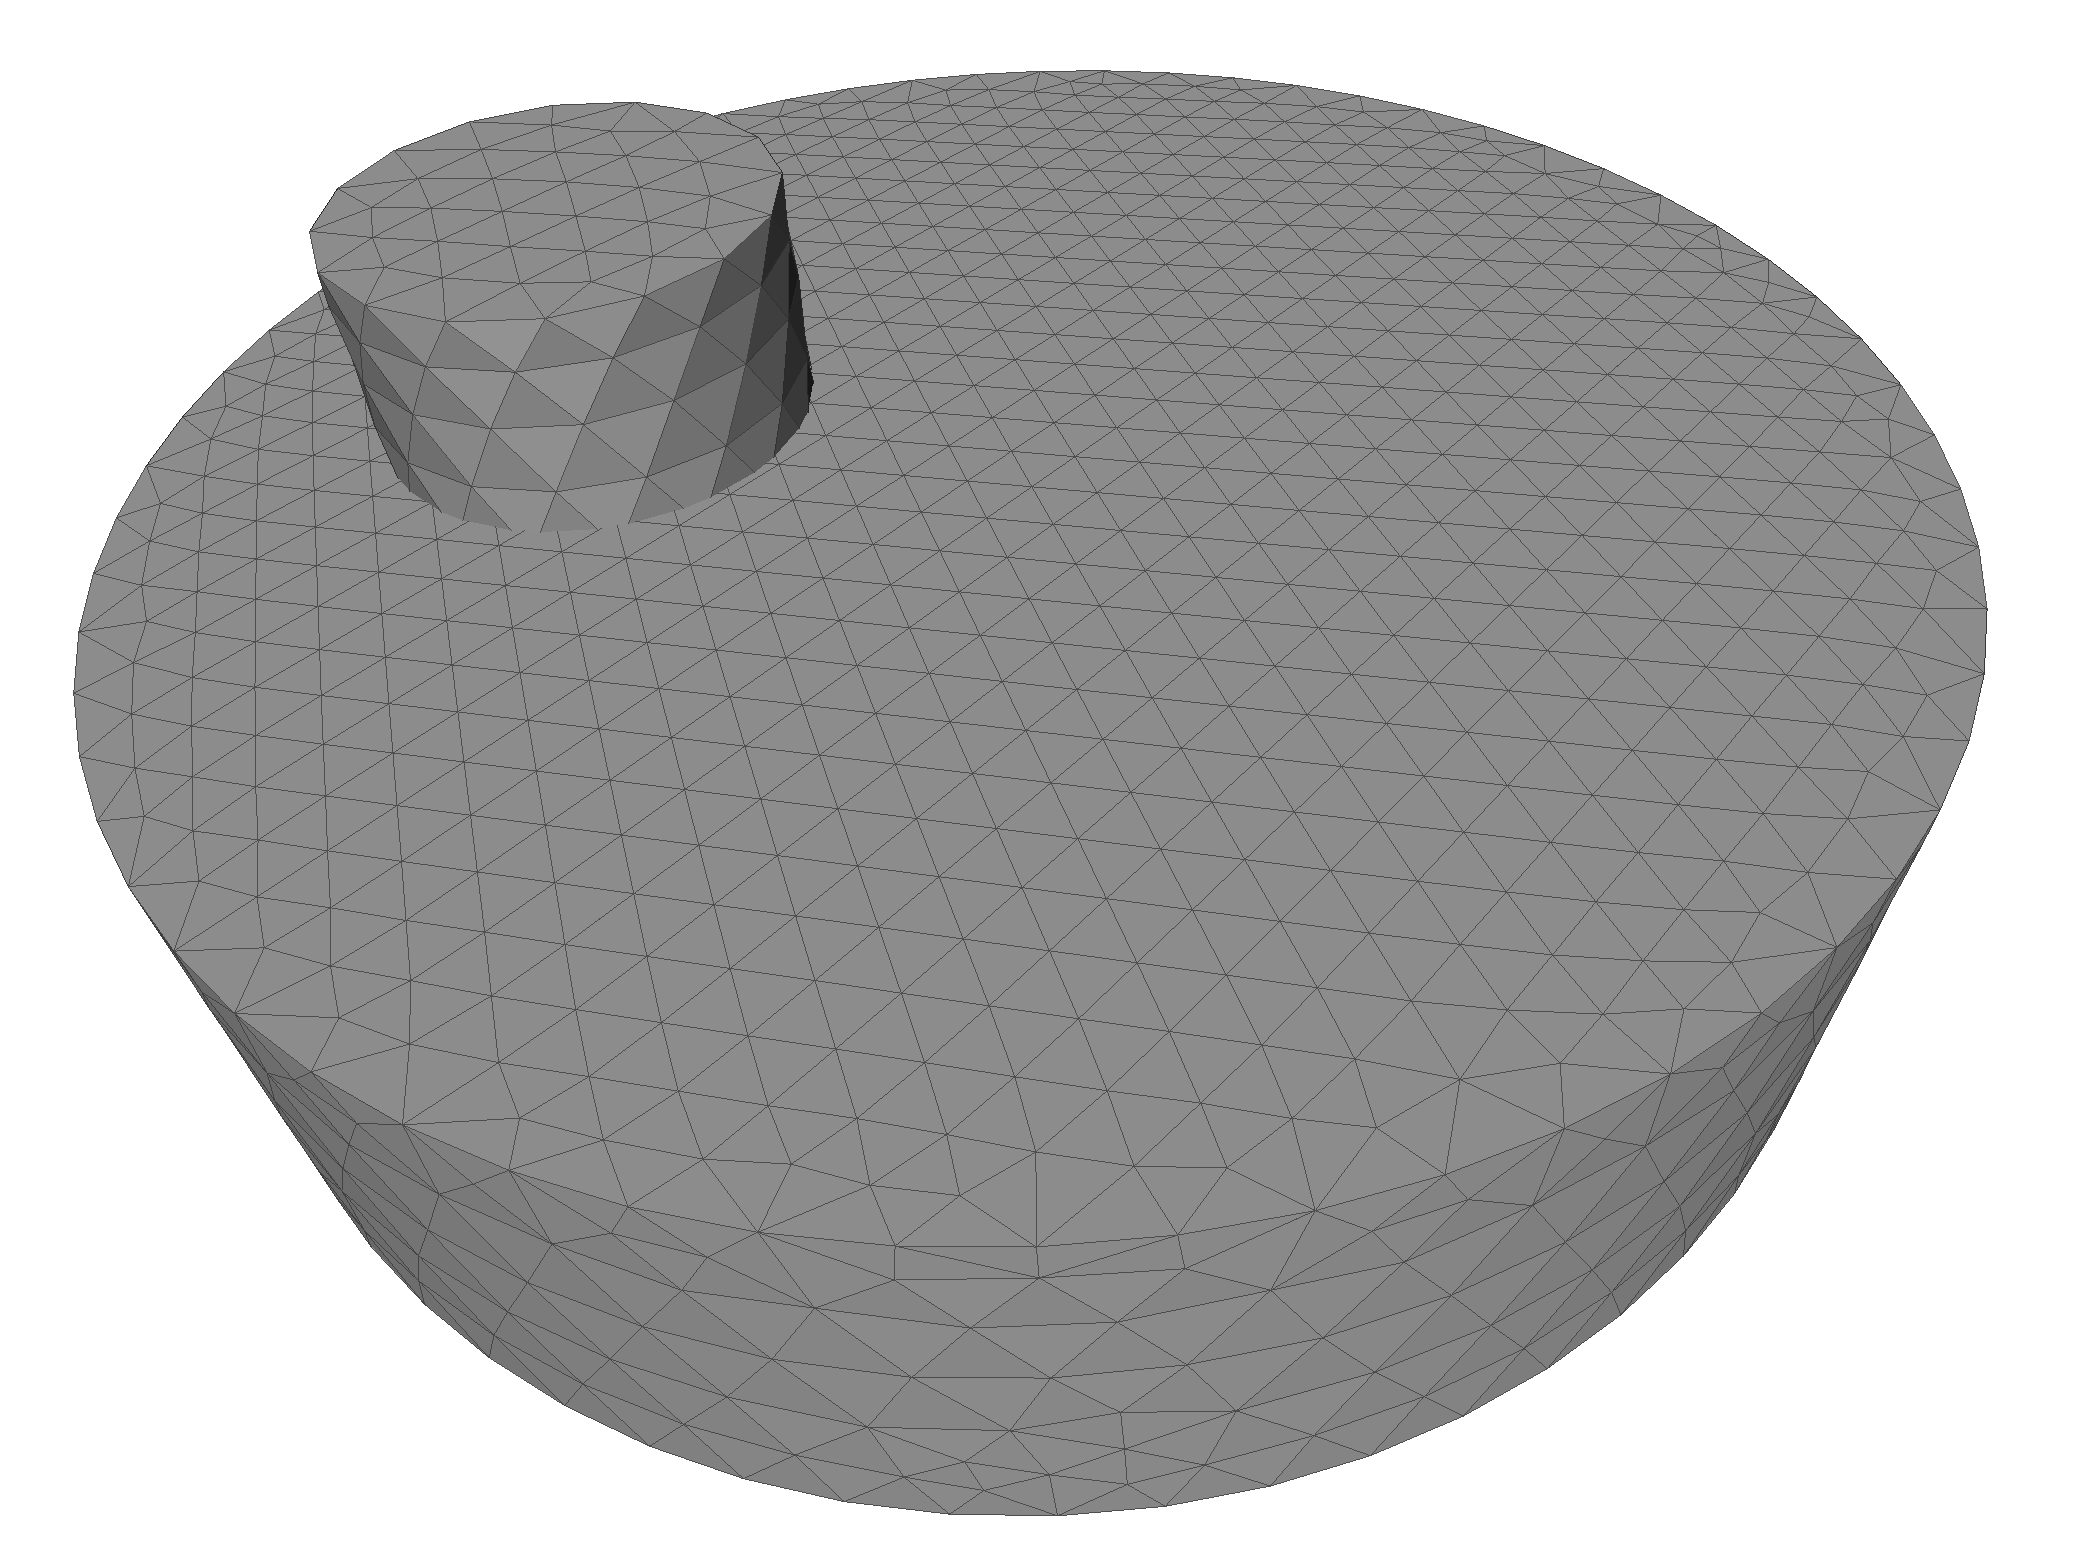
\includegraphics[width=\textwidth]{images/cylinders_classification_before}
		\caption{Before elimination.}
		\label{fig:cylinders_classification_before}
	\end{subfigure}
	\begin{subfigure}[b]{0.4\textwidth}
		\centering
		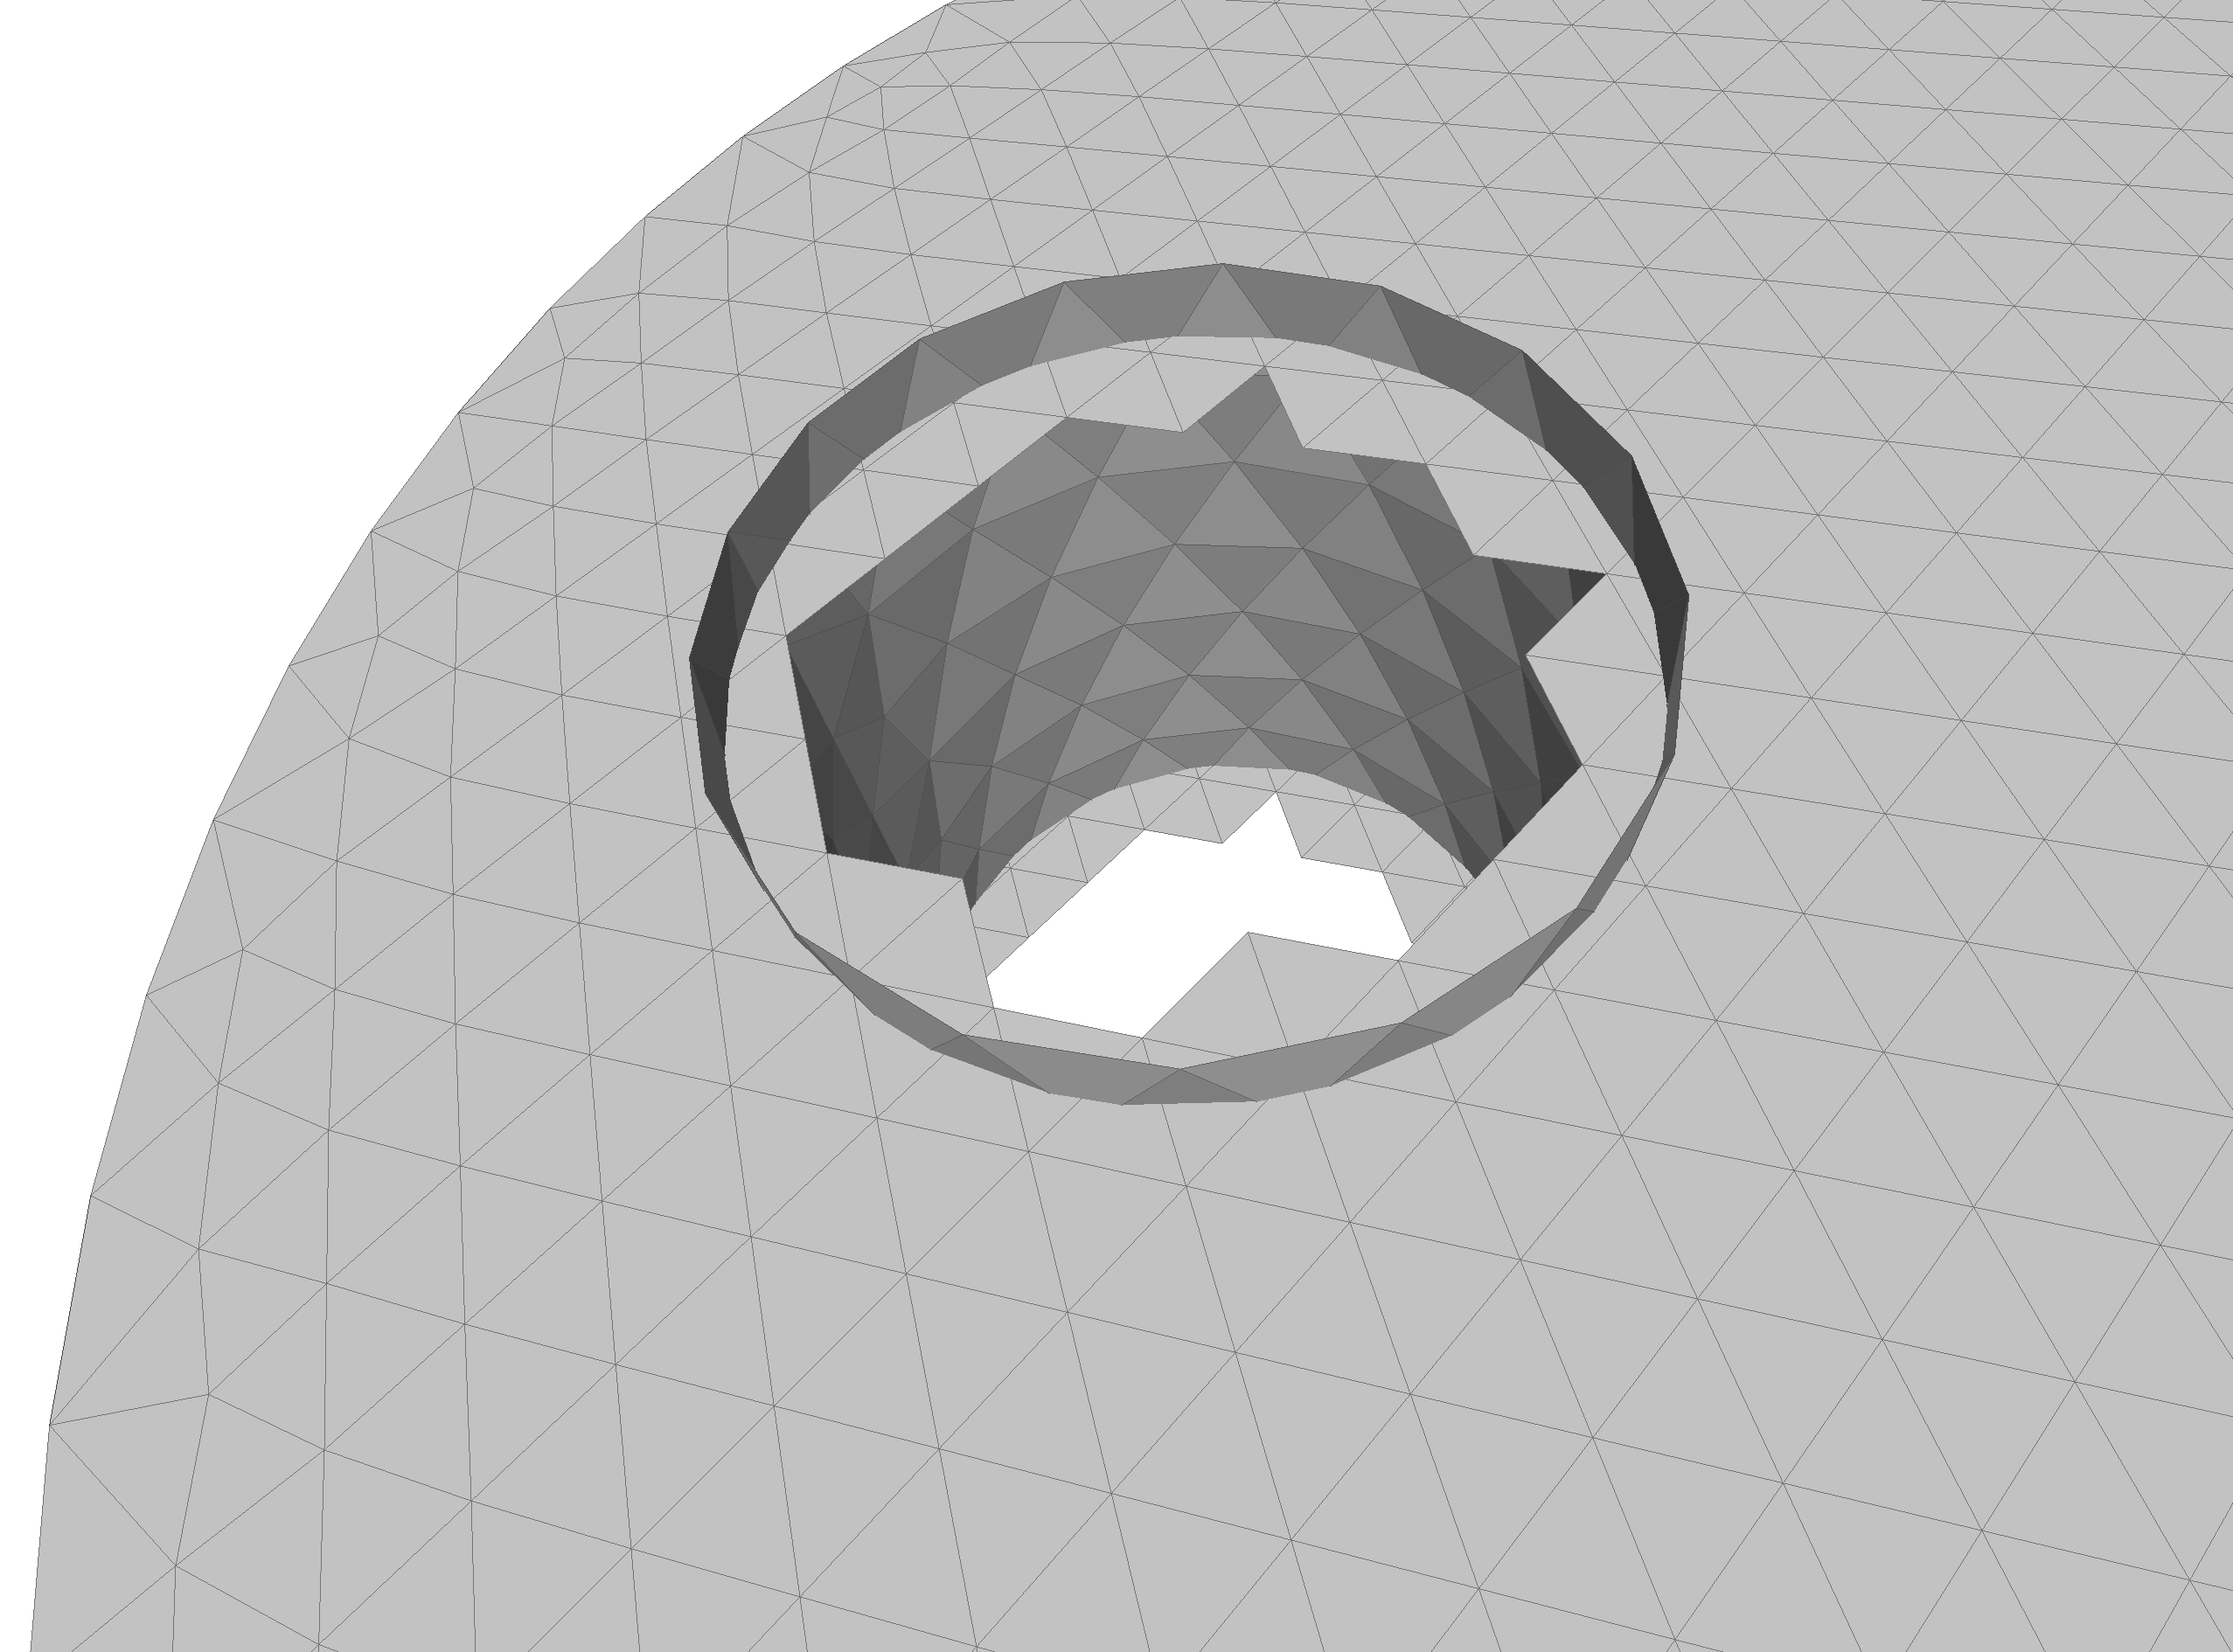
\includegraphics[width=\textwidth]{images/cylinders_classification_after}
		\caption{After elimination.}
		\label{fig:cylinders_classification_after}
	\end{subfigure}
	\caption[Triangle elimination]{
		Scene of a cylindrical stock with a smaller cylindrical swept volume.
		The left image shows both meshes before triangle elimination.
		The right image shows the resulting geometry after triangle elimination.
		Both meshes are no longer closed.
	}
	\label{fig:cylinders_classification}
\end{figure}


\subsection{Visualization by raycasting}
\label{sec:raycasting}

The VML's regular grid with its open geometries resulting from classification are visualized using an adapted raycasting approach.
For this purpose a virtual camera is placed relative to the regular grid.
The camera's position and orientation describe an image plane, \ie a rectangle, in front of the camera which will correspond to the final image.
Originating from the camera's position, a ray is sent through each pixel of the image plane into the scene.
If an intersection occurs, the pixel associated with the ray is colored according to properties of the intersected surface, \eg color, normal and material.
\Cref{fig:raycasting_principle} shows the basic principle of raycasting inside the VML.

\begin{figure}
	\centering
	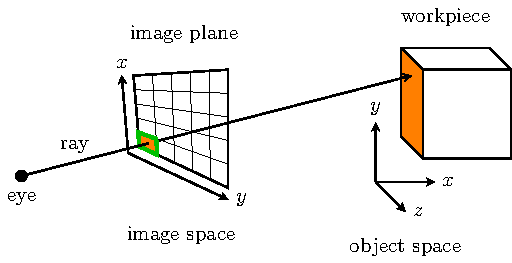
\includegraphics[width=0.7\textwidth]{raycasting}
	\caption[Raycasting principle]{
		Principle of raycasting.
		A ray is sent from an eye point, \ie camera position, through each pixel of an image plane and is traversed through the scene containing the workpiece.
		If an intersection occurs, the pixel is colored according to the intersected surface, \protect\eg color of the surface, lighting using the normal of the surface or material parameters.
		\cite{enlight_demo_workshop}.
	}
	\label{fig:raycasting_principle}
\end{figure}

When the rays hit the regular grid, they have to be traversed through the grid's cells.
A fast algorithm for traversing regular grids using a single ray is found in literature \cite{3DDDA}.
The algorithm is a slight modification of the digital differential analyzer (DDA) which is used for the rasterization of lines.
\Cref{fig:cell_traverser} shows a sketch of a single ray traversed cell by cell through the grid.
%
As neighboring rays typically take the same or a similar path through the grid, grouping rays into ray packets has been proposed as a good optimization \cite{packet_caster}.
This approach has been implemented for the VML using CPU SIMD vector extensions like SSE and AVX  \cite{enlight} and the Intel Xeon Phi many-core architecture.
\Cref{fig:slice_traverser} shows a sketch of a ray packet traversed slice by slice through the grid.

\begin{figure}
	\centering
	\begin{subfigure}[t]{0.44\textwidth}
		\centering
		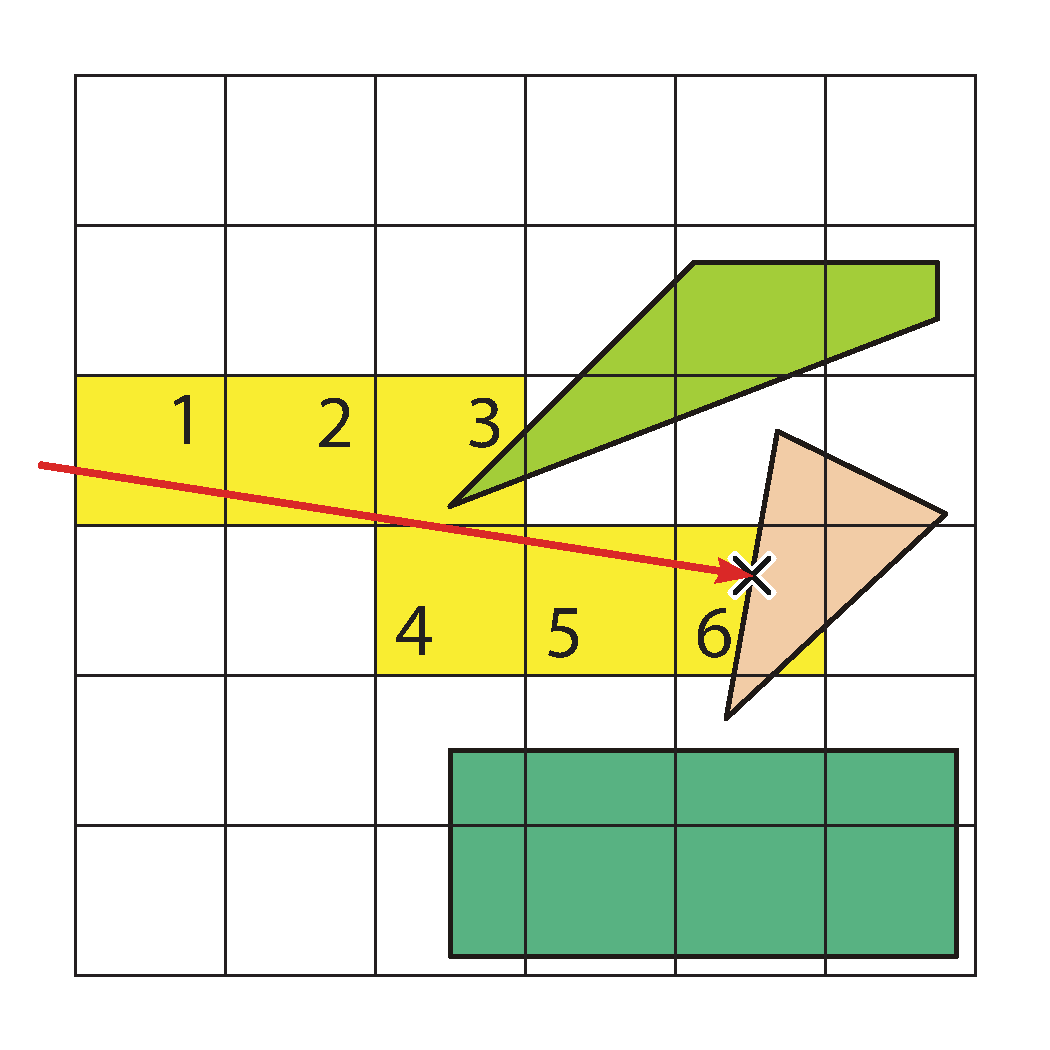
\includegraphics[width=\textwidth]{images/cell_traverser}
		\caption{Single ray.}
		\label{fig:cell_traverser}
	\end{subfigure}
	\begin{subfigure}[t]{0.44\textwidth}
		\centering
		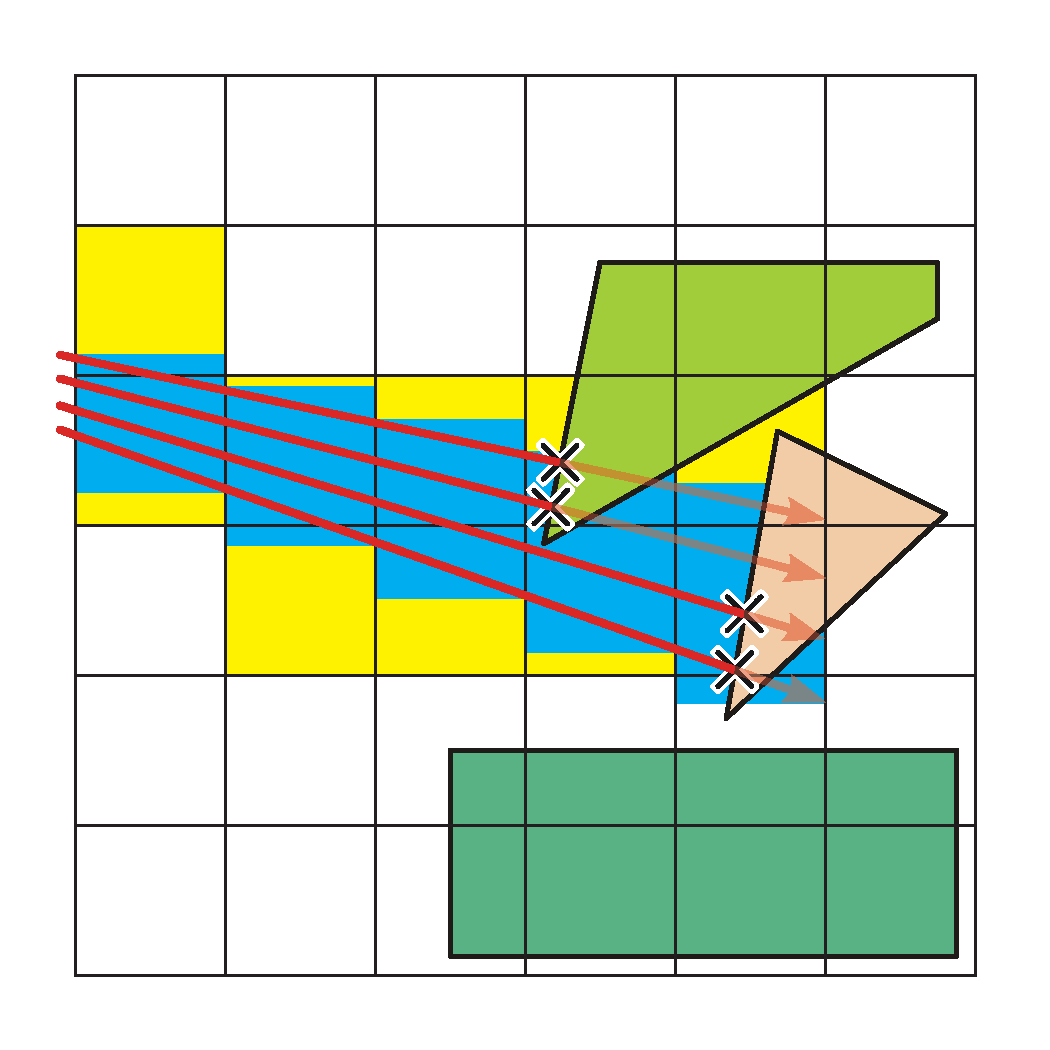
\includegraphics[width=\textwidth]{images/slice_traverser}
		\caption{Ray packet.}
		\label{fig:slice_traverser}
	\end{subfigure}
	\caption[Single ray and ray packet traverser]{
		Traversing a regular grid with a single ray, cell by cell, left image, and a ray packet, slice by slice, right image.
	}
	\label{fig:traverser}
\end{figure}

Cells classified as outside or inside are empty, \ie contain no triangles, but each surface cell contains triangles which can potentially intersect the ray.
A surface cell also typically contains parts, \ie meshes, of multiple swept volumes which are called structures in the context of a cell.
Upon entry into a surface cell, the ray has to determined the number of structures, \ie swept volumes, the ray's entry point is inside of.
This number is called the inside counter.
The stock volume is handled specially during the raycast, as it is inverted and turned into a swept volume itself to allow uniform handling.
After the inside counter has been determined, all intersections of the ray with structures inside the cell are iterated from the nearest to the farthest.
During this iterating the inside counter is modified on each structure entry or exit to constantly reflect the number of structures the ray is currently inside.
If the counter becomes zero, the surface has been reached and a hit is reported with data from the hit triangle which is later used to color the final image of the scene.
\Cref{fig:raycast} shows a detailed example of such an intersection procedure and explains the algorithmic steps to retrieve the surface hit.

\begin{figure}
	\centering
	\begin{subfigure}[t]{0.44\textwidth}
		\centering
		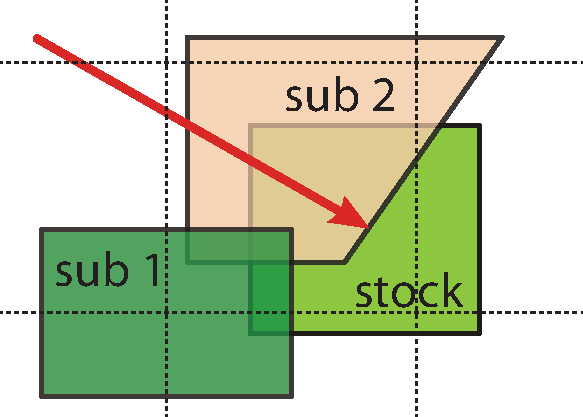
\includegraphics[width=\textwidth]{images/raycast_grid}
		\caption{Conceptual raycast.}
		\label{fig:raycast_grid}
	\end{subfigure}
	~
	\begin{subfigure}[t]{0.44\textwidth}
		\centering
		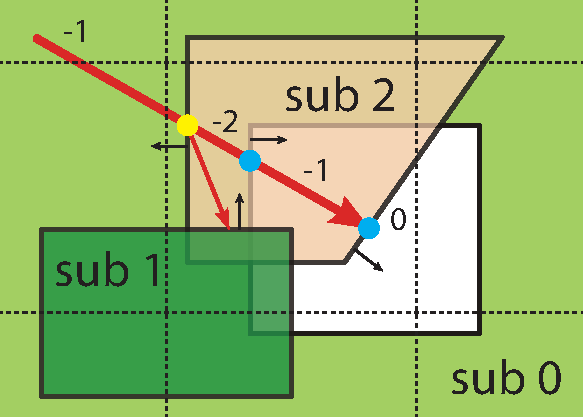
\includegraphics[width=\textwidth]{images/raycast_inside_counter}
		\caption{Implementation of raycast.}
		\label{fig:raycast_inside_counter}
	\end{subfigure}
	\caption[Raycasting interiors]{
		Interiors of the raycasting implementation.
		Upon cell entry, the inside counter is determined.
		Firstly, all intersections of the ray with structures inside the cell are calculated.
		The ray hits the structures sub 0 and sub 2.
		The surface normal of the nearest hit point with sub 2 points into a different half space than the ray direction.
		Therefore, the ray is outside sub 2 upon entry.
		The normal of the nearest hit point with sub 0 points into the same half space than the ray direction.
		Thus, the ray is inside sub 0 at the entry point.
		As the ray does not hit sub 1, a secondary ray is sent to a reference point on a triangle of sub 1.
		As the normal of sub 1 points into a different half space than the secondary ray, the ray is outside sub 1.
		Consequently, as the ray is only inside one structure, sub 0, the inside counter is initialized with -1.
		Then, all previously calculated intersections of the primary ray are ordered ascendingly by distance to the cell entry point and iterated over.
		At each intersection point, the surface normal is again compared with the ray direction.
		If they point into the same half space the structure is exited, otherwise entered.
		Entries decrease the inside counter and are marked with a yellow dot.
		Exists increase the inside counter and are marked with a blue dot.
		When the counter reaches zero, the surface point has been found.
	}
	\label{fig:raycast}
\end{figure}


\subsection{Regular grid interface}
\label{sec:vml_implementation}

To allow the extraction methods presented in this thesis to interface with the regular grid data structure, a few implementation details are needed.
This information conceptually reflects the actual implementation, providing a simplified but sufficient abstraction.

The regular grid data structure relies on a few classes shown in \cref{fig:vml_datamodel}.
The \var{RegularGrid} class basically stores a bit of meta data together with a large set of cells.
The meta data consists of the grid's axis-aligned bounding box (AABB), \var{aabb}, the size of a cell in one dimension, \var{cellSize}, as well as the number of cells in each dimension, \var{cellCount}.
The grid's cells are stored linearized in a flat array.

An axis-aligned bounding box is represented by the \var{Extends} class.
It stores two vertices, \var{lower} and \var{upper}, which contain the minimum and maximum values for each Cartesian coordinate axis.

The cells of the regular grid are modeled by the \var{Cell} class.
Each cell contains its own bounding box, \var{aabb}, the classification of the cell, \var{classification}, and an array of the triangles contained within this cell, \var{triangles}.

Each triangle, described by the class \var{Triangle}, stores its three vertices in counterclockwise order in the member \var{vertices}.
Additionally, the normal of the triangle is stored in \var{normal}, computed from the triangle's vertices for performance reasons.
Especially intersection tests, \eg during raycasting or classification, read this field very frequently and benefit from precomputation.
Each triangle also stores an unsigned integer, \var{structure}, referencing the swept volume/structure this triangle belongs to.
This field is used to group triangles inside a cell by the swept volume they originated from.

Finally, the \var{Vertex} class represents a simple 3-dimensional spatial point, storing the coordinates in its \var{values} member.

\begin{figure}
	\centering
	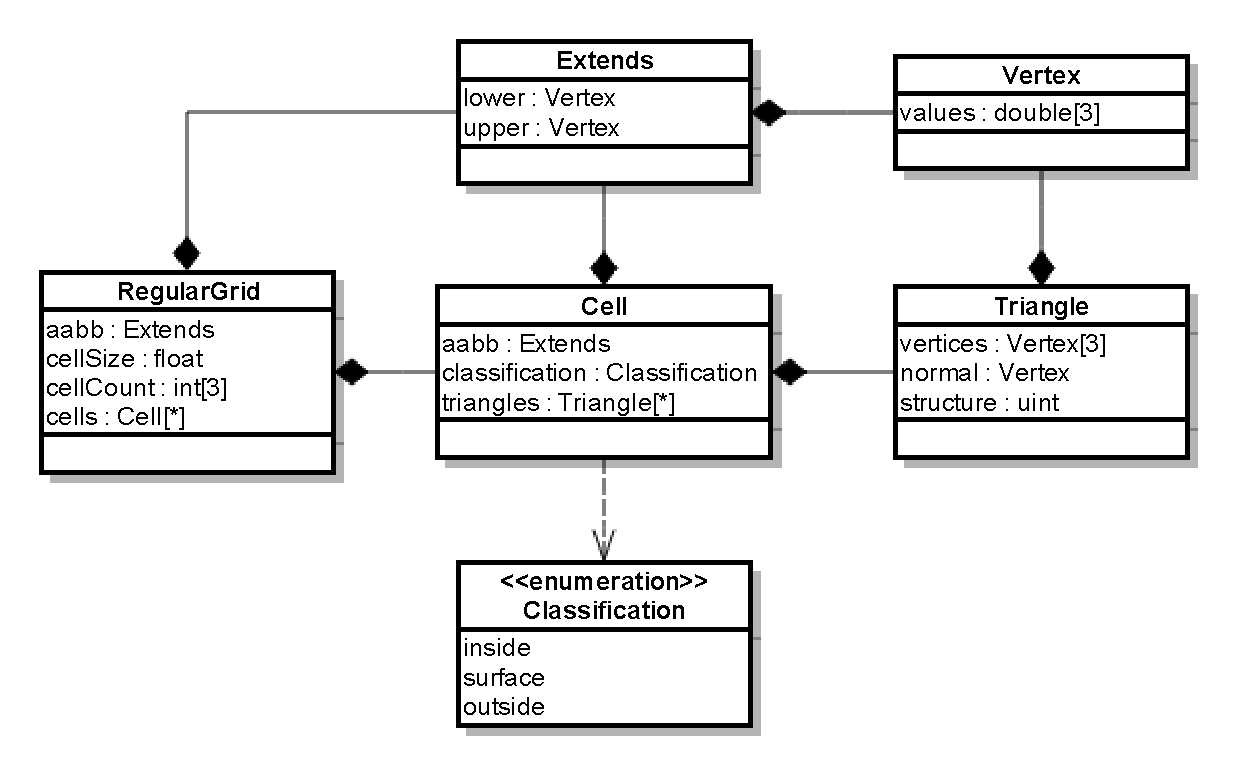
\includegraphics[width=0.9\textwidth]{vml_datamodel}
	\caption[VML UML class diagram]{
		Simplified UML class diagram of the VML data model.
	}
	\label{fig:vml_datamodel}
\end{figure}


\chapter{Related work and state of the art}
\label{ch:state_of_the_art}

Algorithms for transforming solid representations as well as surface reconstruction algorithms are used in a variety of fields:
From 3D artist tools for virtual sculpting and triangle exporters of CAD software to surface reconstruction from real world laser scans.
In the context of this thesis, the scope of solid representation transformation and surface reconstruction is limited to the field of virtual machining and triangulated manifold outputs.
After a survey of existing approaches to surface reconstruction from models similar to the one of the VML, at least four different classes of algorithms have been identified:

\begin{description}
	\item[Direct intersection] \hfill \\
	Directly intersecting each volume with each other, triangle by triangle, is the most direct and theoretically exact approach of calculating the result of a series of Boolean subtractions.
	A good description of triangle mesh intersections is given by Rosen who tried to smooth the sharp intersection line between two meshes to improve the visual impression in video games \cite{mesh_intersection}.
	Triangle-triangle intersection is described by Möller \cite{tri_tri_intersection_moller} as well as Tropp \etal \cite{tri_tri_intersection_2}.

	To build a new surface mesh from two intersecting ones, each intersected triangle can be split into polygons based on the cut segments from other triangles and retriangulated using the cutting segments as constraints.
	A possible solution for this retriangulation is the CDT and was first described by Chew \cite{cdt} and refined by Sloan \cite{cdt_fast}.
	After retriangulating intersected triangles, all triangles not belonging to the new surface are removed.
	A very similar approach is described by Gong \cite{cutter_workpiece_engagement}.


	\item[Point cloud based] \hfill \\
	Point clouds are data structures where an object is approximated by a set of points with optional normal vectors.
	These points are obtained by sampling the surface of a solid, either virtually using a raycast or in reality by scanning the surface of an object, \eg laser scans of buildings or sculptures.
	The VML already uses surface sampling of its data model via its raycast based visualization.
	%
	Point clouds can be triangulated using different algorithms:

	Edelsbrunner \etal present a generalization of the convex hull called $\alpha$-shape \cite{alpha_shape}, which constructs a Delaunay triangulation of the surface described by a set of points.
	The algorithm is subject to a configured $\alpha$ which directly influences the amount of generated holes and the quality of features.

	Based on the computation of Voronoi diagrams and medial axes, Amenta \etal present the crust and power crust algorithm for reconstructing Delaunay triangulations from point clouds with certain quality guarantees, \eg water-tightness, for \enquote{good} inputs \cite{crust, power_crust}.
	Amenta \etal further introduce the cocone algorithm \cite{cocone} which is extended by Dey \etal with tight cocone, robust cocone and recently singular cocone \cite{tight_cocone, robust_cocone, singular_cocone}.
	The crust and cocone families where originally designed to reconstruct surfaces from laser scans and can, partially, handle noise on the input data.

	Hoppe \etal present an algorithm which uses a signed distance function to describe the distance from each point to the estimated surface, \ie functional representation.
	The contour of this function is then traced by a marching cubes variant to extract an isosurface, \ie triangle mesh \cite{sdf_surface_reconstruction}.
	Further algorithms of this class are Poisson \cite{poisson}, moving least squares (MLS) \cite{mls} and radial basis function (RBF) \cite{rbf}.
	As all of these approaches are based on fitting a function into the point cloud, they are robust against noisy clouds, \eg from laser scans.

	Bernardini \etal describe the Ball-Pivoting Algorithm (BPA) for triangulating a point cloud which also contains points inside the cloud which are not relevant for the surface \cite{bpa}.
	Based on the BPA, the G2S algorithm, named after the Gabriel 2-simplex criterion, further improved speed and triangle quality by assuming local surface continuity \cite{g2s}.
	The BPA and its derivatives are region-growing based algorithms and typically provide good runtime performance, but may leave holes in the reconstructed mesh and therefore cannot guarantee water-tight solids.


	\item[Dexel based] \hfill \\
	Dexel representations are widely used in virtual machining as they allow relatively simple Boolean operations.
	Although the data model of the VML stores triangulated manifolds directly, a dexel representation can be easily created based on the existing raycasting system.
	By casting parallel rays through the regular grid of the VML from one side to the other and continuing after a surface intersection, a valid dexel image can be constructed.
	When this process is done along the three axes of the Cartesian coordinate system, a tri-dexel image is obtained.
	A feature conserving algorithm for converting tri-dexel representations into polygon meshes is demonstrated by Ren \etal \cite{tridexel_reconstruction} and guarantees water-tightness.


	\item[Voxel based] \hfill \\
	Enlight already uses a regular grid data structure to organize triangles and classify the cells, \ie voxels, of the grid as inside, outside and surface.
	Therefore, algorithms, which can directly operate on these cells, may profit from the existing infrastructure.
	Although the sole utilization of the classification leaves a lot of information untouched, reconstructing a surface along the surface cells would be a fast way of obtaining a coarse triangle mesh of the stored workpiece.
	By using additional information inside each cell and on each grid point, well known algorithms like marching cubes may be used to retrieve a triangle mesh.
	Kobbelt \etal propose a post-processing step to the marching cubes algorithm to extract and preserve features of the represented surface by making use of triangles, points and implicit functions inside each voxel to construct a scalar distance field, sampled at each grid point \cite{extended_marching_cubes}.
	This algorithm is sometimes also referred to as extended marching cubes.
	The OpenVDB library of DreamWorks Animation uses a similar approach for reconstructing triangle surfaces from large, sparse point clouds organized in octrees with fixed depth \cite{openvdb}.
	The accuracy of this variant can even be further improved using dual contouring as described by Ju \etal \cite{dual_contouring}.
\end{description}


\chapter{Direct intersection method}
\label{ch:direct_intersection}

The first presented method to extract a triangulated surface from the VML's data model is by directly processing the stored triangles inside the VML's regular grid.
This approach is the most straightforward, computationally intensive, but, in theory, most accurate one.
It is conceptually equivalent to directly intersecting the mesh of the stock with each swept volume mesh.
Boolean operations on triangle meshes are already available in most CAD kernels.
However, these kernels usually require the meshes to be closed.
Due to the triangle elimination strategy using cell classification, \cf \cref{sec:classification}, the meshes stored in the regular grid are no longer closed.
Thus, regular CAD kernels cannot be used to intersect the meshes maintained by the VML and a custom mesh intersection algorithm has been developed.
The idea of this approach is based on a work about finding and deforming the intersection between two meshes as well as applying textures to those regions to increase the realism in computer graphics, \ie computer games \cite{mesh_intersection}.

\section{Concept}
\label{sec:direct_intersection_concept}

Every time a swept volume is added to the VML, a unique identifier, \ie a number, is generated and assigned to each of the swept volume's triangles before they are mapped to the cells of the regular grid.
As the stock is internally treated as a swept volume, by inverting the surface normals, all stock triangles are also assigned a unique identifier.
These identifiers allow to separate the triangles contained in the regular grid into the previous swept volumes, referred to as structures.
The identifiers of these structures are called structure ids.

The separated structures are processed in pairs.
Each pair is merged into a new structure.
The union of the two structure meshes is calculated by intersecting each triangle of one mesh with each triangle of the other mesh.
If two triangles intersect, the intersection line is recorded for both triangles.
After intersection, each triangle with intersection lines is split along these lines and retriangulated.
All previous intersection lines are now edges of new triangles.
Each triangle of one structure is then tested against the other structure, whether the triangle is inside or outside the other structure, \eg by casting a ray from the triangle to the other structure.
As all triangles, which initially intersected the opposite structure, have been split, this inside-or-outside property should be unambiguously determinable for each triangle.
By removing all triangles of a structure which are inside the opposite structure, the remaining triangles of both structures form a new surface which corresponds to the union of both structures.
This new structure is then again pairwise united with other structures until only one structure is left, \ie all structures are reduced to one.
This final structure is the reconstructed surface of the VML's data model.
\Cref{fig:cube2} demonstrates this workflow by the example of intersecting a cube with a cuboid.

\begin{figure}
	\centering
	\begin{subfigure}[t]{0.3\textwidth}
		\centering
		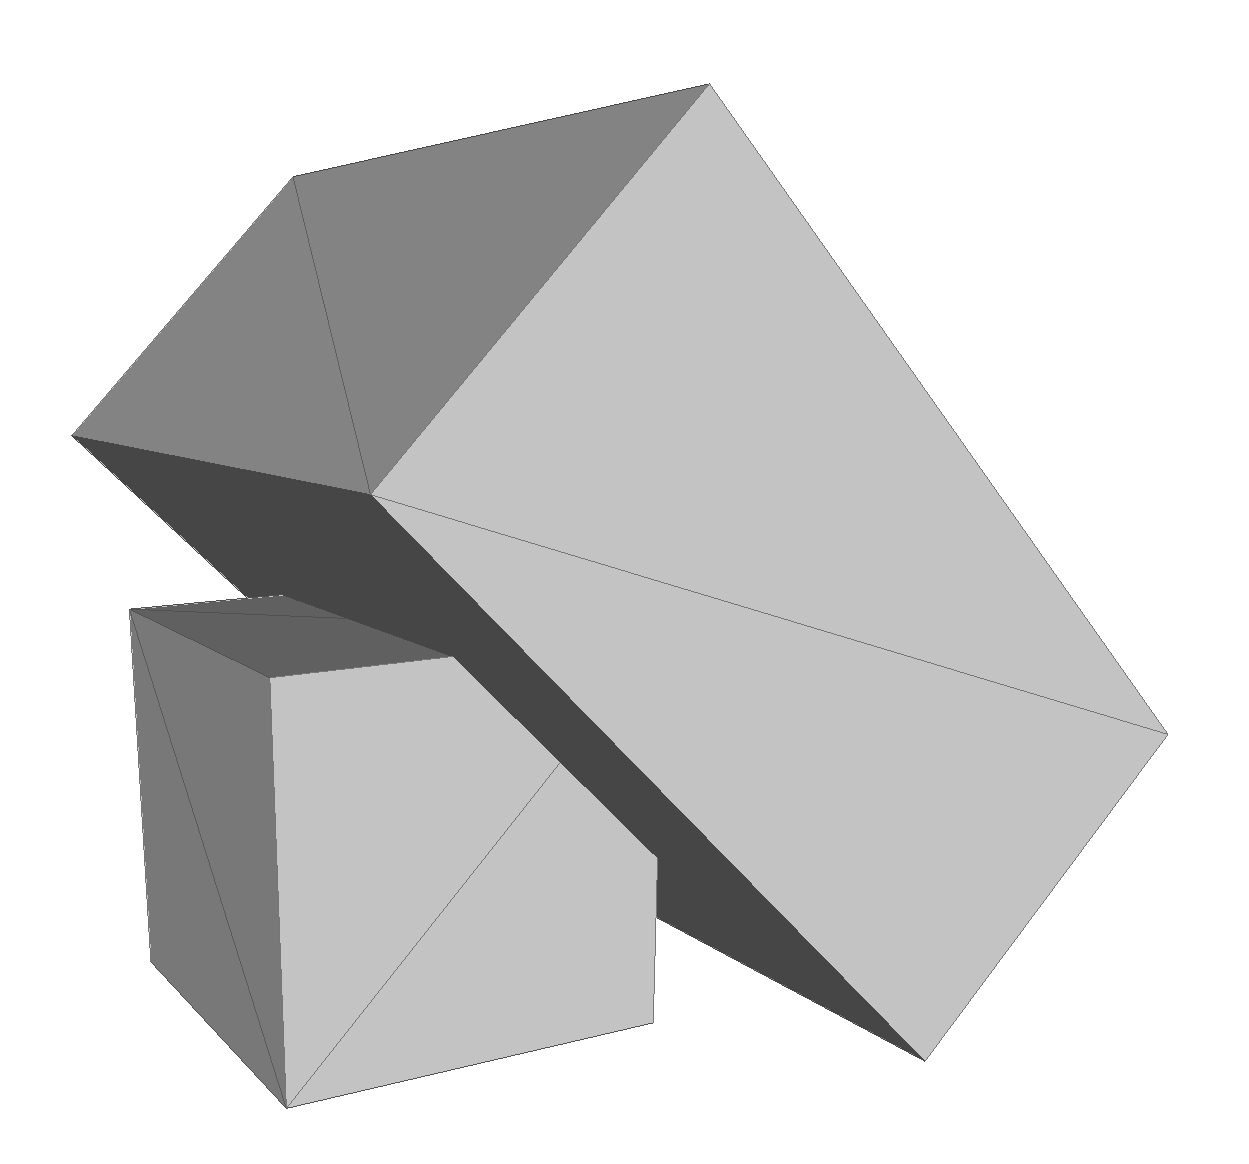
\includegraphics[width=\textwidth]{images/cube2_stock_sv}
		\caption{Stock and SV}
		\label{fig:cube2_stock_sv}
	\end{subfigure}
	\begin{subfigure}[t]{0.3\textwidth}
		\centering
		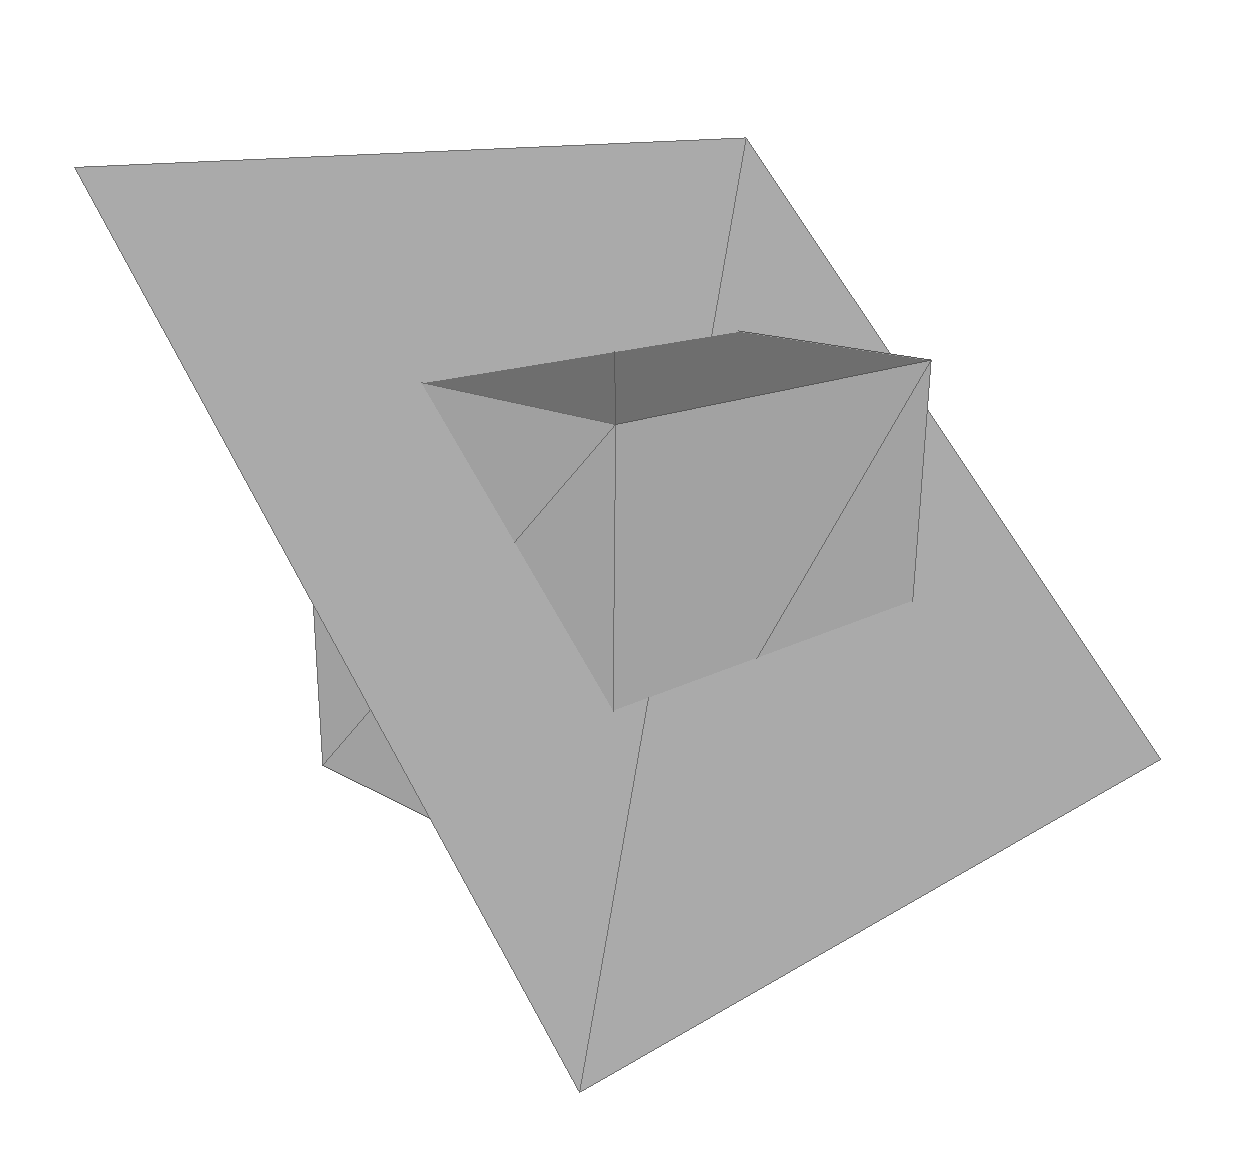
\includegraphics[width=\textwidth]{images/cube2_classified}
		\caption{VML}
		\label{fig:cube2_classified}
	\end{subfigure}
	\begin{subfigure}[t]{0.3\textwidth}
		\centering
		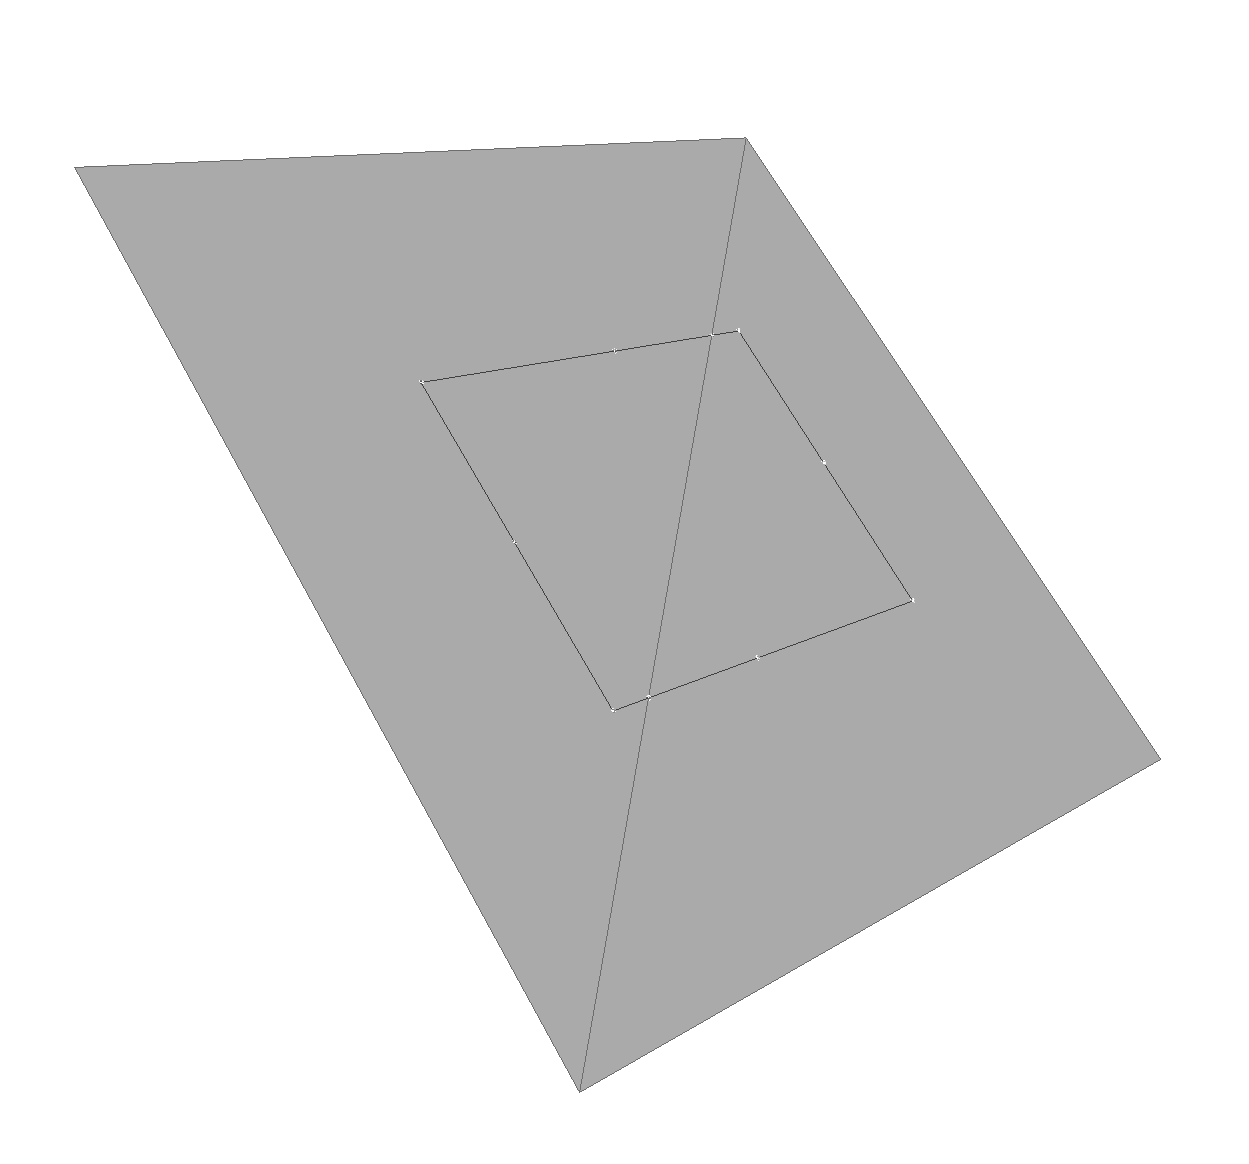
\includegraphics[width=\textwidth]{images/cube2_constraints}
		\caption{Intersections}
		\label{fig:cube2_constraints}
	\end{subfigure}
	\begin{subfigure}[t]{0.3\textwidth}
		\centering
		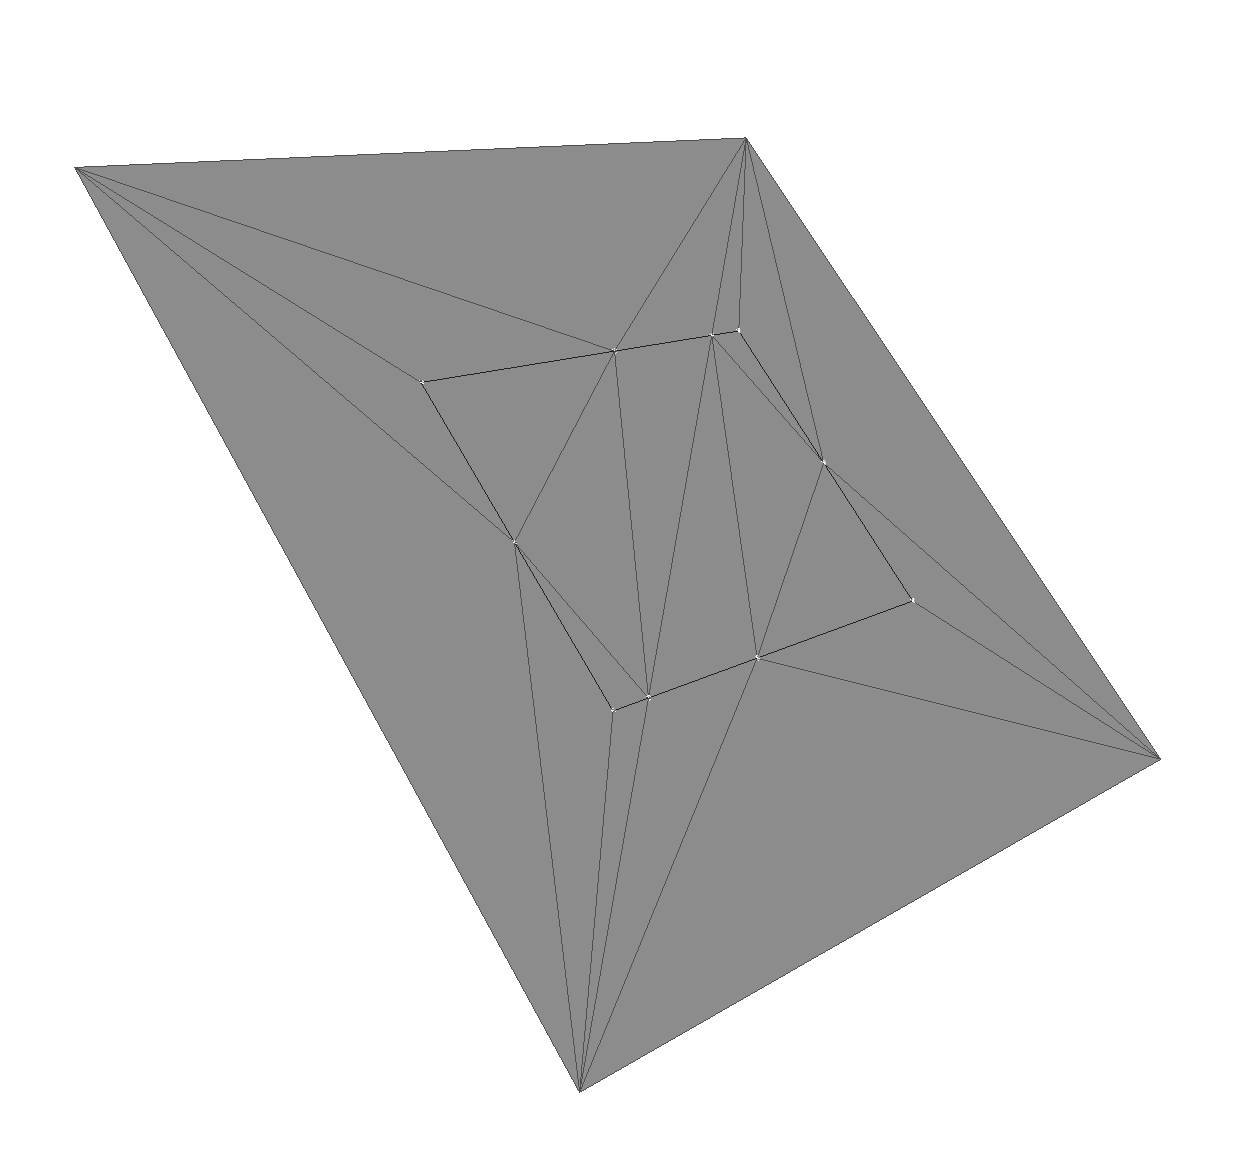
\includegraphics[width=\textwidth]{images/cube2_retriangulated}
		\caption{Retriangulation}
		\label{fig:cube2_retriangulated}
	\end{subfigure}
	\begin{subfigure}[t]{0.3\textwidth}
		\centering
		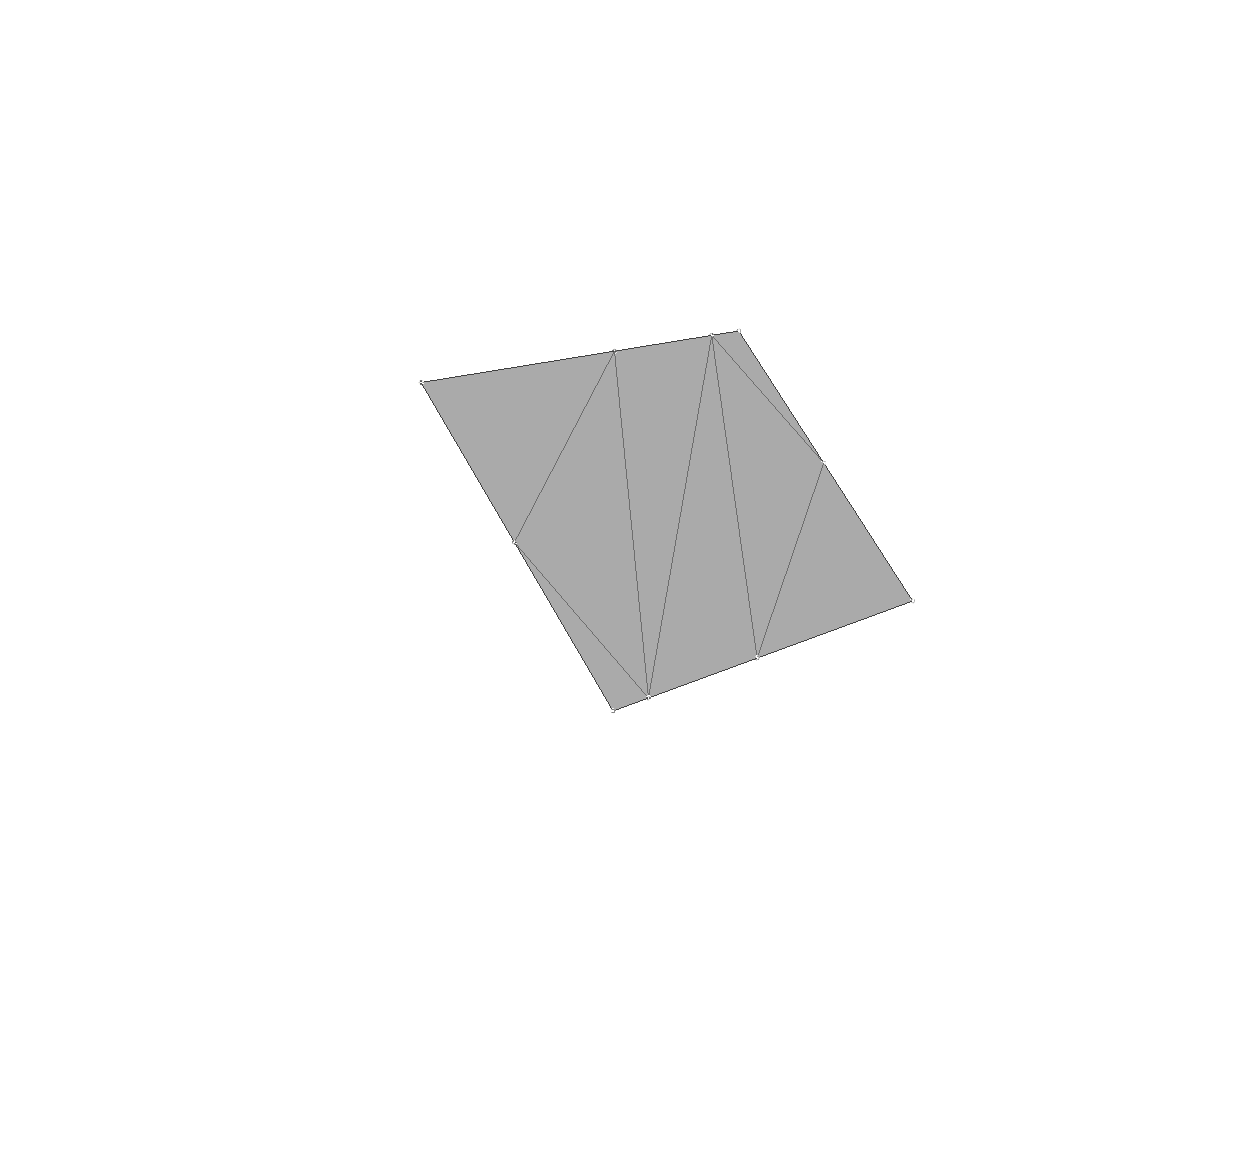
\includegraphics[width=\textwidth]{images/cube2_eliminated}
		\caption{Inside test}
		\label{fig:cube2_eliminated}
	\end{subfigure}
	\begin{subfigure}[t]{0.3\textwidth}
		\centering
		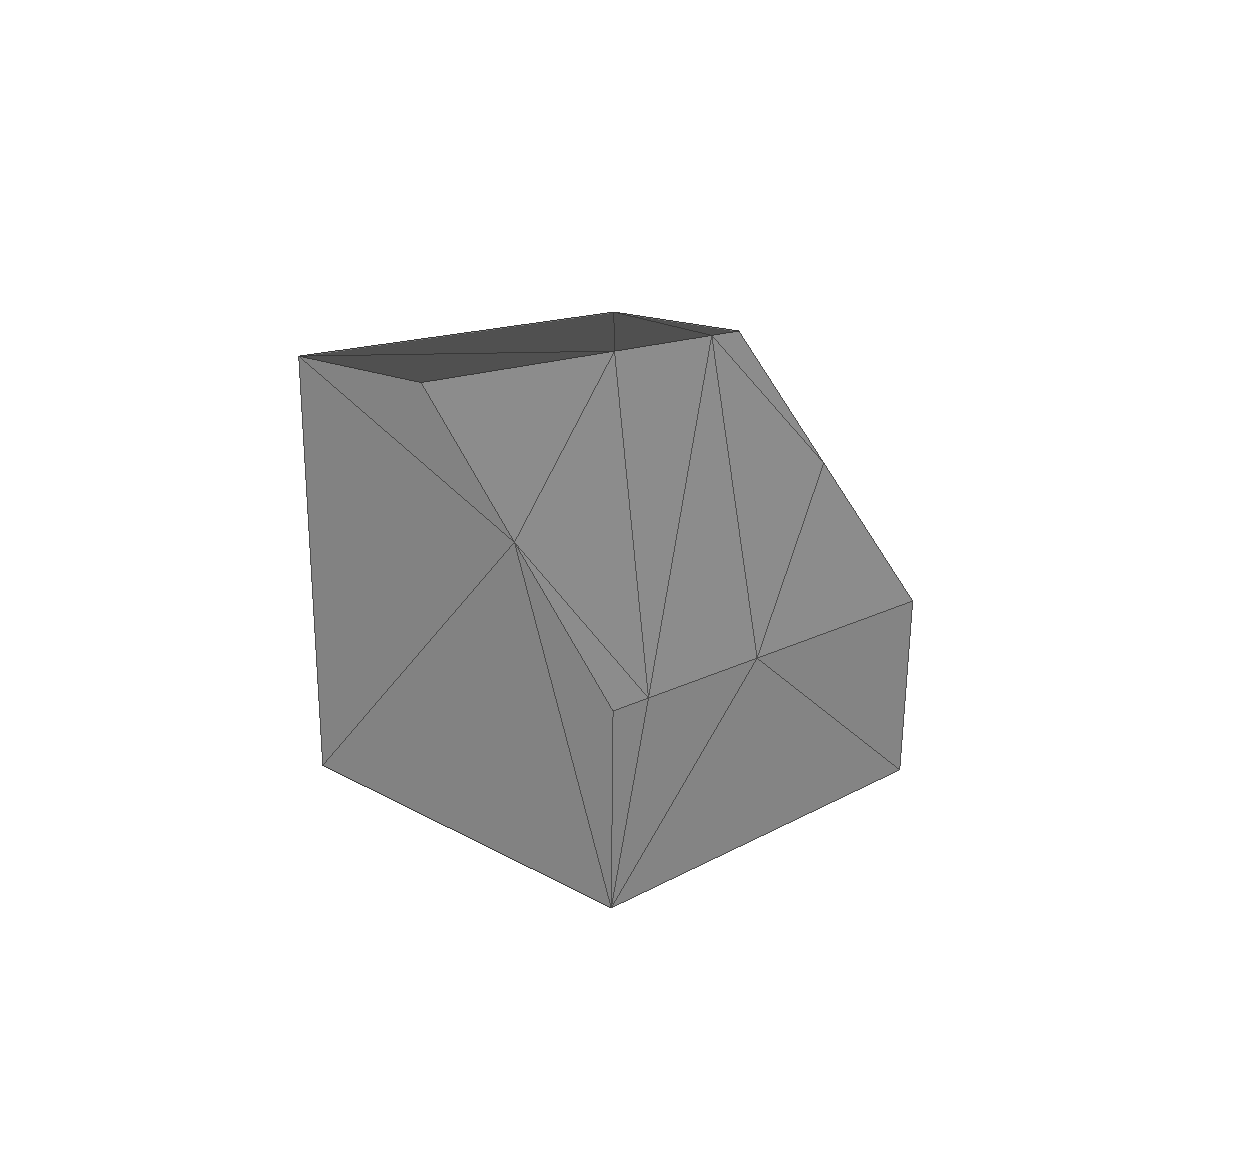
\includegraphics[width=\textwidth]{images/cube2_result}
		\caption{Result}
		\label{fig:cube2_result}
	\end{subfigure}
	\caption[Direct intersection concept]{
		Surface reconstruction from the VML's data model by the example of intersecting a cube and a cuboid.
		The cubic stock, in the lower left, and a tilted cuboid as swept volume, in the upper right, is shown in \subref{fig:cube2_stock_sv}.
		The classification result when these two solids are mapped into the VML's regular grid is shown in \subref{fig:cube2_classified}.
		Most of the swept volume's triangles have been removed.
		When intersecting both structures, \ie swept volume and stock triangles, all intersection lines per triangle are recorded.
		For the swept volume's triangles, \subref{fig:cube2_constraints} shows these lines.
		The triangles are then retriangulated with respect to those intersections as shown in \subref{fig:cube2_retriangulated}.
		Afterwards, each triangle is tested against the other structure, whether they are inside and can be removed.
		The result of testing the retriangulated swept volume's triangles against the stock is shown in \subref{fig:cube2_eliminated}.
		The retriangulation and inside test is analogously done for the stock structure.
		Finally, the reconstructed surface is the union of the remaining triangles, \cf \subref{fig:cube2_result}.
	}
	\label{fig:cube2}
\end{figure}


\section{Implementation}
\label{sec:direct_intersection_implementation}

In general, intersecting each triangle of a structure against each other triangle of another structure is an expensive procedure.
The cost of this operation is $\mathcal{O}(n^2)$, assuming both structures have $n$ triangles.
Intersecting the structures at the level of each cell greatly reduces the value of $n$.
Unfortunately, many triangles usually span the bounding boxes of several cells and are duplicated in each encompassed one.
To avoid duplicates or overlapping triangles when combining results from neighboring cells, all triangles of a cell have to be clipped against the cell's bounding box.
This step can be done before or after intersecting the structures of a cell, but always before starting to eliminate triangles against the opposite structure.
There is also a second reason why this direct intersection approach must be run on a cell level which is discussed in \cref{sec:triangle_inside_test}.

An abstracted algorithm of this reconstruction approach is shown in \cref{alg:direct_intersection}.
The following sections discuss details of this algorithms and follow the order of subroutines/functions used within.
The only exception is the \textproc{SeparateStructures} routine, which only groups the incoming triangles by their structure id.
It returns a list of structures, where each structure is a set of triangles.

\begin{algorithm}
	\centering
	\begin{algorithmic}[1]
		\Function{DirectIntersection}{$\var{grid}$}
			\State $\var{result} \gets \varnothing$
			\ForAll{$\var{cell} \in \var{grid}.\var{cells}$}
				\If{$\var{cell}.\var{classification} = \var{surface}$}
					\State $\var{structures} \gets \Call{SeparateStructures}{\var{cell}.\var{triangles}}$
					\If{$\left\vert{\var{structures}}\right\vert = 1$}
						\State $\var{result} \gets \var{result} \cup \Call{ClipStructure}{\var{structures}.\var{pop}(), \var{cell}.\var{aabb}}$
					\ElsIf{$\left\vert{\var{structures}}\right\vert > 1$}
						\State $\var{acc} \gets \var{structures}.\var{pop}()$
						\While{$\left\vert{\var{structures}}\right\vert > 0$}
							\State $\var{s} \gets \var{structures}.\var{pop}()$
							\State $\var{acc} \gets \Call{UnionStructure}{\var{acc}, \var{s}, \var{cell}.\var{aabb}}$
						\EndWhile
						\State $\var{result} \gets \var{result} \cup \var{acc}$
					\EndIf
				\EndIf
			\EndFor
			\State \Return $\var{result}$
		\EndFunction
		\\
		\Function{UnionStructure}{$\var{s}_1, \var{s}_2, \var{cellBox}$}
			\ForAll{$\var{s} \in \{\var{s}_1, \var{s}_2\}$}
				\State $s \gets \Call{ClipStructure}{\var{s}, \var{cellBox}}$
			\EndFor
			\State $\var{lines} \gets \var{map}()$ \Comment{maps each triangle to a set of lines}
			\ForAll{$(\var{t}_1, \var{t}_2) \in \var{s}_1 \times \var{s}_2$}
				\State $\var{l} \gets \Call{IntersectTriangles}{\var{t}_1, \var{t}_2}$
				\If{$\var{l}$} \Comment{no intersection line may be found}
					\State $\var{lines}(\var{t}_1) \gets \var{lines}(\var{t}_1) \cup \{\var{l}\}$
					\State $\var{lines}(\var{t}_2) \gets \var{lines}(\var{t}_2) \cup \{\var{l}\}$
				\EndIf
			\EndFor
			\ForAll{$\var{s} \in \{\var{s}_1, \var{s}_2\}$}
				\State $\var{s'} \gets \varnothing$
				\ForAll{$\var{t} \in \var{s}$}
					\State $\var{s'} \gets \var{s'} \cup \Call{SplitTriangle}{\var{t}, \var{lines}(\var{t})}$
				\EndFor
				\State $\var{s} \gets \var{s'}$
			\EndFor
			\State $\var{result} \gets \varnothing$
			\ForAll{$(\var{s}, \var{s'}) \in \{(\var{s}_1, \var{s}_2), (\var{s}_2, \var{s}_1)\}$}
				\ForAll{$\var{t} \in \var{s}$}
					\If{$\neg \Call{IsTriangleInsideStructure}{\var{t}, \var{s'}}$}
						\State $\var{result} \gets \var{result} \cup \{\var{t}\}$
					\EndIf
				\EndFor
			\EndFor
			\State \Return $\var{result}$
		\EndFunction
	\end{algorithmic}
	\caption[Direct intersection workflow]{
		Abstract workflow of the surface reconstruction using direct intersection of the VML's stored structures.
	}
	\label{alg:direct_intersection}
\end{algorithm}


\subsection{Clipping}
\label{sec:clipping}

Clipping triangles against the bounding box of a cell is necessary to avoid duplicated or invalid surfaces.
In cases where triangles span multiple cells, the VML duplicates each triangle into each cell it encompasses.
During intersection, only a triangle's intersections with structures of the current cell are recorded, although the triangle might be intersected by additional geometry in neighboring cells.
Therefore, after splitting, parts of the triangle which are outside the current cell are never split, might pass the inside test as a whole and remain as additional triangles outside the actual surface or remain collinear with surface triangles from neighboring cells.
To circumvent these issues, all triangles of a cell have to be clipped either before or after intersecting the two structures in \textproc{UnionStructure}.

Algorithms for clipping triangles against a bounding box are described in literature.
A well-known examples is the Sutherland-Hodgeman algorithm for polygon clipping \cite{polygon_clipping}.
Although further algorithms exist, \eg Weiler-Artherton, Vatti or Greiner-Hormann, which are either faster, more robust or have fewer restrictions on their input, the Sutherland-Hodgeman algorithm is characteristically simple.
In particular, it clips any polygon against any convex clip polygon by iteratively clipping it against infinitely extended lines along each edge of the clip polygon.
Despite being initially designed for two dimensions, the algorithm easily extends to higher dimensions.

For clipping triangles against the bounding box of a cell, a 3-dimensional version of the Sutherland-Hodgeman algorithm is needed.
\Cref{alg:clip} shows a pseudocode implementation of the \textproc{ClipStructure} routine which is based on the Sutherland-Hodgeman algorithm to clip all structure triangles against the bounding box of a cell.
%
When clipping a structure against a bounding box, each individual triangle of the structure is clipped separately.
The result of clipping a single triangle may be the same triangle, a set of new triangles or even no triangle at all.
The resulting triangles after clipping, if any, are collected to form the new, clipped structure.

The Sutherland-Hodgeman algorithm clips against a convex polygon, or its equivalent in higher dimensions, \ie a polytope, by iteratively clipping against each side.
In case of a bounding box, the input polygon has to be clipped against each of the six sides of the cell.
These sides are extended and described as planes by specifying a normal vector and the plane's distance to the origin.
The six planes built from a cell's bounding box are given in the \textproc{ClipPolygonAABB} function of \cref{alg:clip}.
The input polygon itself is represented as an ordered list of vertices, where each pair of adjacent vertices form an edge of the polygon, including the last and the first vertex as a pair.
The order of the vertices remains the same during the clipping process, but vertices may be removed or additional ones added.
The final vertex list, after clipping against all planes, needs to be triangulated again.
As the clipping volume, \ie the cell's bounding box, is convex, the resulting clipped polygon is also convex.
Therefore, the list of vertices can be simply triangulated into a fan by selecting one vertex and emitting a triangle for every adjacent pair of vertices excluding the selected vertex, where each triangle is built from the pair and the selected vertex.
Note that in some edge cases, duplicate vertices may be generated.
Thus, duplicates should be removed from the result vertex list before passing it to the triangulation subroutine.

The core routine of the clipping procedure is clipping the list of vertices against a single plane.
Initially, an empty list of result vertices is created.
For each of the polygon's vertices, the signed distance to the clipping plane is calculated.
The distance of each vertex is compared with the distance of its preceding vertex.
If the signs of the distances are different, the edge represented by the current vertex and its predecessor intersects the clipping plane.
In this case, the intersection point with the clipping plane is calculated, \cf \cref{alg:clip} for details, and the point is added to the result list.
If the distance of the current vertex is positive, the vertex itself is inside the clipping volume and is also added to the result list.
After all vertices have been processed, the result list is return, representing the clipped polygon again as an ordered list of its vertices.

\begin{algorithm}
	\centering
	\begin{algorithmic}[1]
		\Function{ClipStructure}{$\var{s}, \var{aabb}$}
			\State $\var{s'} \gets \varnothing$
			\ForAll{$\var{t} \in \var{s}$}
				\State $\var{s'} \gets \var{s'} \cup \Call{ClipPolygonAABB}{\var{t}.\var{vertices}, \var{aabb}}$
			\EndFor
			\State \Return $\var{s'}$
		\EndFunction
		\\
		\Function{ClipPolygonAABB}{$\var{vertices}, \var{aabb}$}
			\State $\var{vertices} \gets \Call{ClipPolygonPlane}{\var{vertices}, \var{Vertex}( 1, 0, 0), \var{aabb}.\var{lower}.\var{x}}$
			\State $\var{vertices} \gets \Call{ClipPolygonPlane}{\var{vertices}, \var{Vertex}(-1, 0, 0), \var{aabb}.\var{upper}.\var{x}}$
			\State $\var{vertices} \gets \Call{ClipPolygonPlane}{\var{vertices}, \var{Vertex}( 0, 1, 0), \var{aabb}.\var{lower}.\var{y}}$
			\State $\var{vertices} \gets \Call{ClipPolygonPlane}{\var{vertices}, \var{Vertex}( 0,-1, 0), \var{aabb}.\var{upper}.\var{y}}$
			\State $\var{vertices} \gets \Call{ClipPolygonPlane}{\var{vertices}, \var{Vertex}( 0, 0, 1), \var{aabb}.\var{lower}.\var{z}}$
			\State $\var{vertices} \gets \Call{ClipPolygonPlane}{\var{vertices}, \var{Vertex}( 0, 0,-1), \var{aabb}.\var{upper}.\var{z}}$

			\State \Return $\Call{Trianglulate}{\Call{Unique}{\var{vertices}}}$
		\EndFunction
		\\
		\Function{ClipPolygonPlane}{$\var{vertices}, \var{n}, \var{d}$}
			\State $\var{result} \gets \var{array}()$
			\State $\var{prev} \gets |\var{vertices}| - 1$
			\State $\var{prevDist} \gets \var{vertices}_\var{prev} \cdot \var{n} - \var{d};$
			\For{$\var{i} \gets 0 \To |\var{vertices}| - 1$}
				\State $\var{dist} \gets \var{vertices}_\var{i} \cdot \var{n} - \var{d}$;
				\If{$(\var{dist} < 0 \wedge \var{prevDist} \geq 0) \vee (\var{dist} \geq 0 \wedge \var{prevDist} < 0)$}
					\State $\var{edge} \gets (\var{vertices}_\var{i} - \var{vertices}_\var{prev})$
					\State $\var{edge} \gets \var{edge} \cdot (\var{dist} \div (\var{n} \cdot \var{edge}))$
					\State $\var{v} \gets \var{vertices}_\var{i} - \var{edge}$
					\State $\var{result}.\var{add}(\var{v})$
				\EndIf
				\If{$\var{dist} \geq 0$}
					\State $\var{result}.\var{add}(\var{vertices}_\var{i})$
				\EndIf
				\State $\var{prev} \gets i$
				\State $\var{prevDist} \gets \var{dist}$
			\EndFor
			\State \Return $\var{result}$
		\EndFunction
		\\
		\Function{Triangulate}{$\var{vertices}$}
			\State $\var{result} \gets \varnothing$
			\If{$|vertices| \geq 3$}
				\State $\var{c} \gets \var{vertices}_0$
				\For{$\var{i} \gets 2 \To |\var{vertices}| - 1$}
					\State $\var{result} \gets \var{result} \cup \{\var{Triangle}(\var{c}, \var{vertices}_{\var{i} - 1}, \var{vertices}_\var{i})\}$
				\EndFor
			\EndIf
			\State \Return $\var{result}$
		\EndFunction
	\end{algorithmic}
	\caption[Sutherland-Hodgeman variant]{
		A Sutherland-Hodgeman algorithm variant for clipping polygons against a bounding box in three dimensions.
	}
	\label{alg:clip}
\end{algorithm}



\subsection{Triangle intersection}
\label{sec:triangle_intersection}

Every time the union surface of two structures is calculated, each triangle of one structure has to be intersected with each triangle of the other structure.
Triangle-triangle intersection is a common problem in collision detection and has been solved numerous times.
The intersection test of Möller \cite{tri_tri_intersection_moller}, despite being older and marginally slower than more recent developments \cite{tri_tri_intersection_2}, is also available as public domain C code on the authors website \cite{tri_tri_intersection_moller_code}.
As only a few adaptations were necessary, Möller's code was taken and thoroughly refactored to fit a modern C++ style without changing its behavior.
Since the code is quite long and freely available on Möller's website, an implementation/algorithm is not included here.
The \textproc{IntersectTriangle} routine referenced in \cref{alg:direct_intersection} is thus merely a small adapter calling into Möller's code and is given in \cref{alg:triangle_intersection}.

\begin{algorithm}
	\centering
	\begin{algorithmic}[1]
		\Function{IntersectTriangles}{$\var{t}_1, \var{t}_2$}
			\State $\var{hasIntersected} =$ \Call{tri\_tri\_intersect\_with\_isectline}{$\hfill\break
				% the phantoms at the line starts make sure all hspaces start at the same position
				\protect\vphantom{p}\hspace*{\dimexpr\algorithmicindent*2}\var{t}_1.\var{vertices}_0, \var{t}_1.\var{vertices}_1, \var{t}_1.\var{vertices}_2,\hfill\break
				\protect\vphantom{p}\hspace*{\dimexpr\algorithmicindent*2}\var{t}_2.\var{vertices}_0, \var{t}_2.\var{vertices}_1, \var{t}_2.\var{vertices}_2,\hfill\break
				\protect\vphantom{p}\hspace*{\dimexpr\algorithmicindent*2}\out\var{isCoplanar}, \out\var{p}_1, \out\var{p}_2$} \Comment{Output parameters}
			\If{$\var{hasIntersected} \wedge \neg \var{isCoplanar}$}
				\State \Return $(\var{p}_1, \var{p}_2)$ \Comment{Otherwise return nothing}
			\EndIf
		\EndFunction
	\end{algorithmic}
	\caption[Möller's triangle-triangle intersection adapter]{
		Adapter to the Möller's triangle intersection routine provided as public domain C code on his website \cite{tri_tri_intersection_moller_code}.
		This algorithm calls the C function \textproc{tri\_tri\_intersect\_with\_isectline} with all triangle vertices as inputs and $\var{coplanar}$, $\var{p}_1$ and $\var{p}_2$ as output parameters.
	}
	\label{alg:triangle_intersection}
\end{algorithm}

The triangle intersection test itself starts with an early exit test by computing the plane equation parameters, \ie normal and distance, for both triangles.
Then, the signed plane distance of each vertex of one triangle to the plane of the other triangle is calculated.
If the signs of these three values is the same for one triangle, it completely lies on one side of the plane and therefore does not intersect the other triangle.
This test is run for both triangles.
Afterwards, the intersection line between the two planes is calculated by crossing the planes' normal vectors.
\Cref{fig:tri_intersect} shows the intersection line of the two triangle planes in green and is used to discuss the remaining part of the algorithm.
Now, the intervals of the line which lie inside the triangle have to be calculated.
For each pair of vertices of a triangle, \ie each triangle's edges, the two signed distances of the vertices to the plane of the other triangle are compared.
If they have a different sign, this edge intersects the other triangle's plane and therefore crosses the intersection line of both planes.
The intersection point splits the edge with the same ratio as the signed distances of both vertices.
For each triangle, two intersecting edges are found, thus yielding an interval for each triangle, \cf blue segments of the line in \cref{fig:tri_intersect}.
If these two intervals overlap, the triangles intersect and their intersection line is the overlapping segment of the planes' intersection line, \cf red segment in \cref{fig:tri_intersect}.
Otherwise, there is no intersection.

\begin{figure}
	\centering
	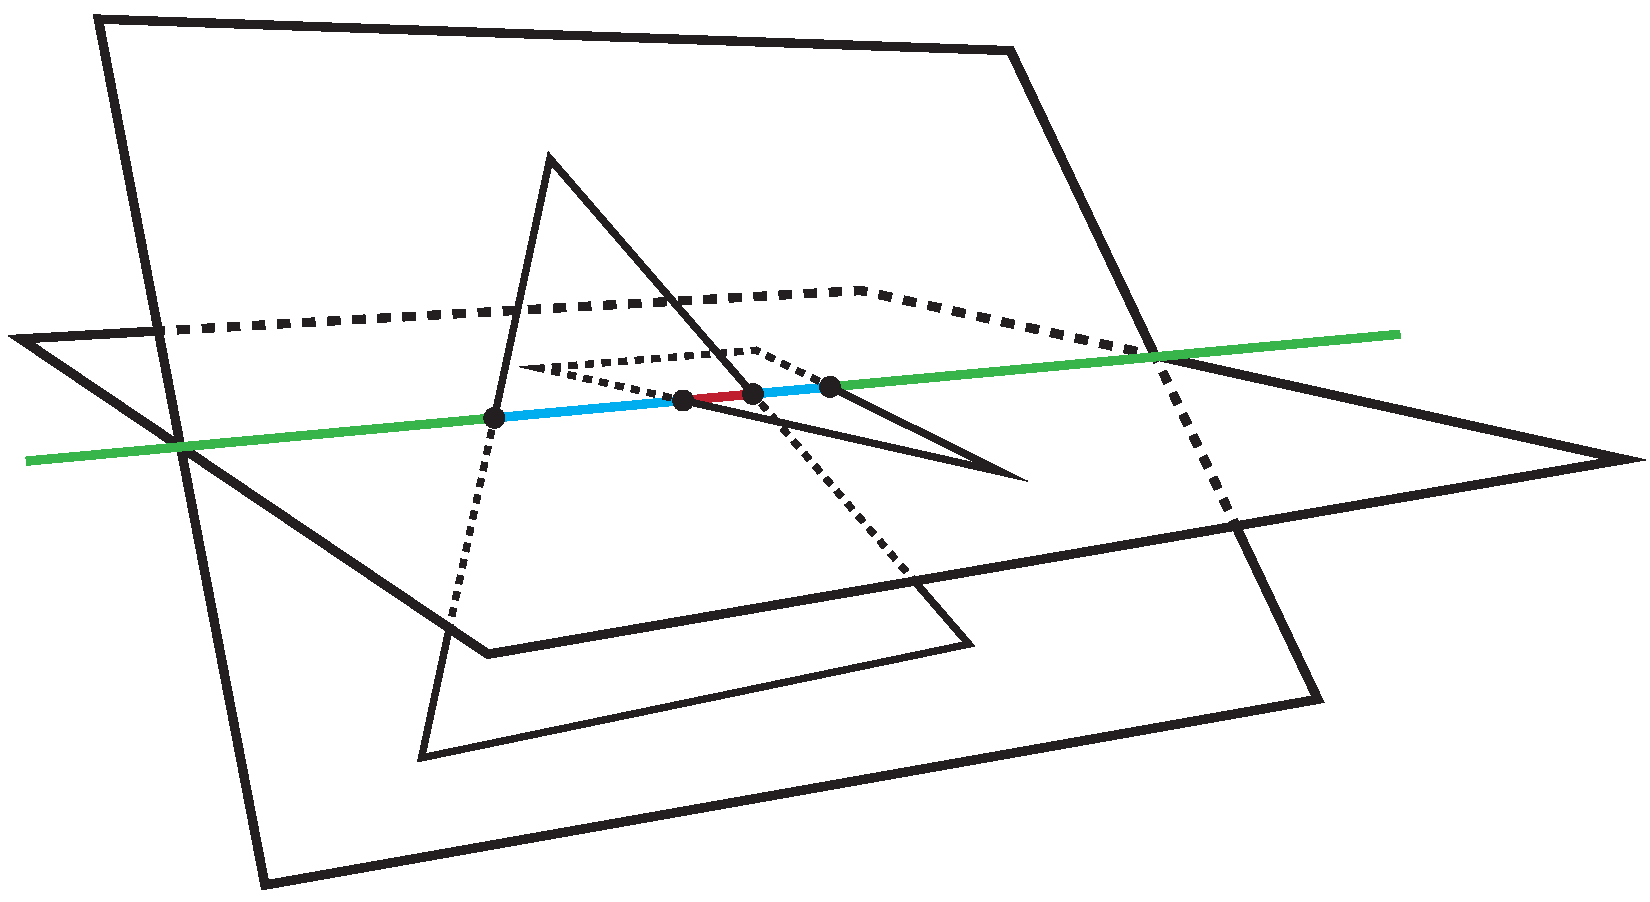
\includegraphics[width=0.8\textwidth]{tri_intersect}
	\caption[Möller triangle-triangle intersection test]{
		Intersection line calculation in Möller's triangle intersection test.
		The image shows intervals on the intersection line between two triangle's planes.
		The green line is the intersection line of both planes.
		Blue parts of the intersection line are intervals of one triangle.
		The red part is the overlap of both triangle's line intervals, \ie the triangle's intersection.
		Image modeled after \cite[p757]{tri_tri_intersection_moller_image}.
	}
	\label{fig:tri_intersect}
\end{figure}

Extending beyond this concept, a further optimization is to do not use the planes' intersection line to project the triangle's intervals onto, but to use the coordinate system's axis where the intersection line's direction has the largest magnitude.
This greatly simplifies several calculations except the actual points of the intersection segment.
Furthermore, Möller's code additionally handles the case when both triangles are coplanar, \ie the signed distances of the vertices of one triangle to the other triangle's plane are almost zero.



\subsection{Triangle splitting}
\label{sec:triangle_splitting}

After two structures have been intersected and all intersection lines per triangle have been recorded, the triangles can be split.
The result of splitting a triangle must be a new set of triangles in order to create a new structure from these which can be put into the \textproc{UnionStructure} routine again.
Hence, an algorithm for triangulating a triangle with respect to a set of lines is needed.
In the context of triangulations, this set of lines is usually called constraints or constrained edges and the according algorithm a constrained triangulation (CT).
Initially, a manually written CT was used.
Even though it was capable of triangulating simple cases, it suffered severely from numerical instability and poor output quality.
A stricter triangulation of higher quality is the constrained Delaunay triangulation (CDT), which is also suggested by the work giving the initial idea to the direct intersection reconstruction approach \cite{mesh_intersection}.
However, as CDT algorithms are quite hard to implement regarding speed and robustness, using an established and tested library is highly recommended.
A list of C/C++ libraries offering constrained Delaunay triangulations is given in \cref{tbl:delaunay_libs}.
Several of these libraries have been tested for their suitability to retriangulate a triangle with a set of constraints.
Usually, these triangulation algorithms operate on 2-dimensional point clouds with optional constrained edges between points of this cloud.
As output they generate a Delaunay triangulation, with the convex hull of the point cloud as boundary.

\renewcommand{\arraystretch}{1.5} % row spacing
\begin{table}[h]
	\centering
	\begin{tabular}{p{3cm} l l p{2.1cm} p{3.9cm}}
		Library                                          &                           & Language & License                                  & Notes                                                             \\
		\midrule
		poly2tri                                         & \cite{poly2tri}           & C++      & BSD                                      & Constrains via polylines must not touch each other                \\
		Triangle                                         & \cite{triangle_lib}       & C        & Custom, free for non-commercial use      & Difficult interface and memory management                         \\
		Geometric Tools Engine (GTE)                     & \cite{gte}                & C++      & Boost License                            & modern C++11, SIMD and GPGPU support, high standard documentation \\
		Computational Geometry Algorithms Library (CGAL) & \cite{cgal_triangulation} & C++      & LGPL, GPL or commercial                  & Huge functionality, de-facto standard in academics                \\
		Fade2D                                           & \cite{fade2d}             & C++      & Commercial, free for scientific research & Closed source                                                     \\
		Triangulation Template Library (TTL)             & \cite{ttl}                & C++      & GPL                                      & Supports usage of own data structures via C++ templates           \\
		GNU Triangulated Surface Library (GTS)           & \cite{gts}                & C        & LGPL                                     & object-oriented design using GLib                                 \\
	\end{tabular}
	\caption[CDT libraries]{
		Several libraries offering a constrained Delaunay triangulation.
	}
	\label{tbl:delaunay_libs}
\end{table}
\renewcommand{\arraystretch}{1.0}

The poly2tri library requires constraints to be specified as polylines which may not touch each other.
This is a problem as constraints may touch the boundary of the original triangle.

The Triangle library is used for splitting triangles at various constrained edges in another work \cite{mesh_intersection}.
Nevertheless, it has a very difficult C interface which tries to mimic a command line with text arguments even on its API level.
Furthermore, passing in and returning geometric data structures requires extensive care regarding memory management.
The library does not reliably work for all triangulation cases and sometimes crashes.

The Geometric Tools Engine (GTE) is a rather modern library with an excellent C++ interface.
The algorithms' precision may be configured via templates.
The library runs outstandingly stable with only a few troubles in cases where the input was numerically problematic, \eg contained points with differences only at the last few digits representable with double precision.
However, these issues can be fixed with appropriate preprocessing of the input, \cf \cref{sec:numeric_improvements}.
Furthermore, the GTE library is licensed under the Boost License and therefore perfectly usable in commercial products like the VML.

The remaining libraries have not been further tested, mainly for the reason that the VML is a commercial product and the use of these libraries would require to drop the code again later.

The integration of the GTE's CDT is done inside \textproc{SplitTriangle} which is given in \cref{alg:triangle_splitting}.
%
\begin{algorithm}
	\centering
	\begin{algorithmic}[1]
		\Function{SplitTriangle}{$\var{t}, \var{lines}$}
			\State $\var{points} \gets \{\var{t}.\var{a}, \var{t}.\var{b}, \var{t}.\var{c}\}$ \Comment{Ordered set}
			\ForAll{$(\var{p}_1, \var{p}_2) \in \var{lines}$}
				\State $\var{points} \gets \var{points} \cup \{\var{p}_1, \var{p}_2\}$
			\EndFor
			\State $\var{axis}_0 \gets \Call{LargestAxis}{\var{t}.\var{normal}}$
			\State $\var{axis}_1 \gets (\var{axis}_0 + 1) \bmod 3$
			\State $\var{axis}_2 \gets (\var{axis}_0 + 2) \bmod 3$
			\State $\var{points2} \gets \varnothing$ \Comment{Project 3D to 2D points, order must remain}
			\ForAll{$\var{p} \in points$}
				\State $\var{points2} \gets \var{points2} \cup \{\var{Vector2}(\var{p}_{\var{axis}_1}, \var{p}_{\var{axis}_2})\}$
			\EndFor
			\State $\var{cdt} \gets \var{ConstrainedDelaunay2()}$
			\ForAll{$(\var{p}_1, \var{p}_2) \in \var{lines}$} \Comment{Add constraints}
				\State $\var{cdt}.\var{Insert}((\var{points}.\var{indexof}(\var{p}_1), \var{points}.\var{indexof}(\var{p}_2)), \dots)$
			\EndFor
			\State $\var{cdt}(|\var{points2}|, \var{points2}, \epsilon)$ \Comment{Compute CDT}
			\State $\var{indices} \gets \var{cdt}.\var{GetIndices}()$
			\State $\var{triangles} \gets \varnothing$
			\For{$\var{i} \gets 0 \To |\var{indices}| \div 3 - 1$}
				\State $\var{f} \gets \var{triangle()}$
				\For{$\var{j} \gets 0 \To 2$}
					\State $\var{index} \gets \var{indices}_{3\var{i} + \var{j}}$
					\State $\var{f}_\var{j} = \var{points}_{\var{index}}$
				\EndFor
				%\If{$\var{f.normal} \cdot \var{t.normal} < 0$}
				%	\State $\var{swap}(\var{f.a}, \var{f.b})$ \Comment{Swap two vertices to reverse winding}
				%\EndIf
				\State $\var{triangles} \gets \var{triangles} \cup \{\var{f}\}$
			\EndFor
			\State \Return $\var{triangles}$
		\EndFunction
		\\
		\Function{LargestAxis}{$\var{v}$}
			\If{$\var{v}.\var{x} > \var{v}.\var{y}$}
				\If{$\var{v}.\var{x} > \var{v}.\var{z}$}
					\State \Return $0$
				\Else
					\State \Return $2$
				\EndIf
			\Else
				\If{$\var{v}.\var{y} > \var{v}.\var{z}$}
					\State \Return $1$
				\Else
					\State \Return $2$
				\EndIf
			\EndIf
		\EndFunction
	\end{algorithmic}
	\caption[GTE CDT adapter]{
		Adapter to the CDT routine provided by the GTE library.
		Uses the \var{ConstrainedDelaunay2} class template to generate a CDT for a given triangle and a set of constrained edges.
		The resulting triangulation is returned.
	}
	\label{alg:triangle_splitting}
\end{algorithm}
%
A few preparations are necessary before the CDT subroutine can be called.
All points used by constrained edges must be part of the input point cloud and are therefore added to the point cloud formed by the input triangle's vertices.

Furthermore, as the CDT only runs in two dimensions, all vertices are projected onto the plane spanned by the two coordinate system axes with the smaller magnitude in the triangle's normal vector.
This operation is simple as it only requires the selection of two components of each point and no calculation.
As all constraints as well as the resulting triangulation are specified using indexes into the point cloud, the list containing the 2-dimensional, projected vertices must have the same order as the original point list.
Before starting the triangulation, the constrained edges have to be specified.
Each constraint is inserted by supplying a pair of indexes into the point cloud.
Afterwards, the CDT can be calculated.
The resulting triangulation is specified using a list of indexes.
The length of this list is a multiple of three and each consecutive three indexes form a triangle of the result.
When these indexes are resolved by indexing into the original point cloud, the vertices for the final triangles are obtained.
These triangles are finally returned.


\subsection{Triangle inside structure test}
\label{sec:triangle_inside_test}

After all triangles of two intersecting structures have been split on their intersection lines, all triangles which do not contribute to the union surface, \ie are inside the other structure, have to be removed.
Due to the regular grid's classification, \cf \cref{sec:classification}, triangles might have been removed and, consequently, structures put together from multiple cells of the regular grid may no longer be closed meshes.
As it turns out, the test whether a triangle is inside another structure may fail if the tested structure is not a closed mesh, a common case.
An example of such an issue is shown in \cref{fig:inside_test_error}.
%
\begin{figure}[!]
	\centering
	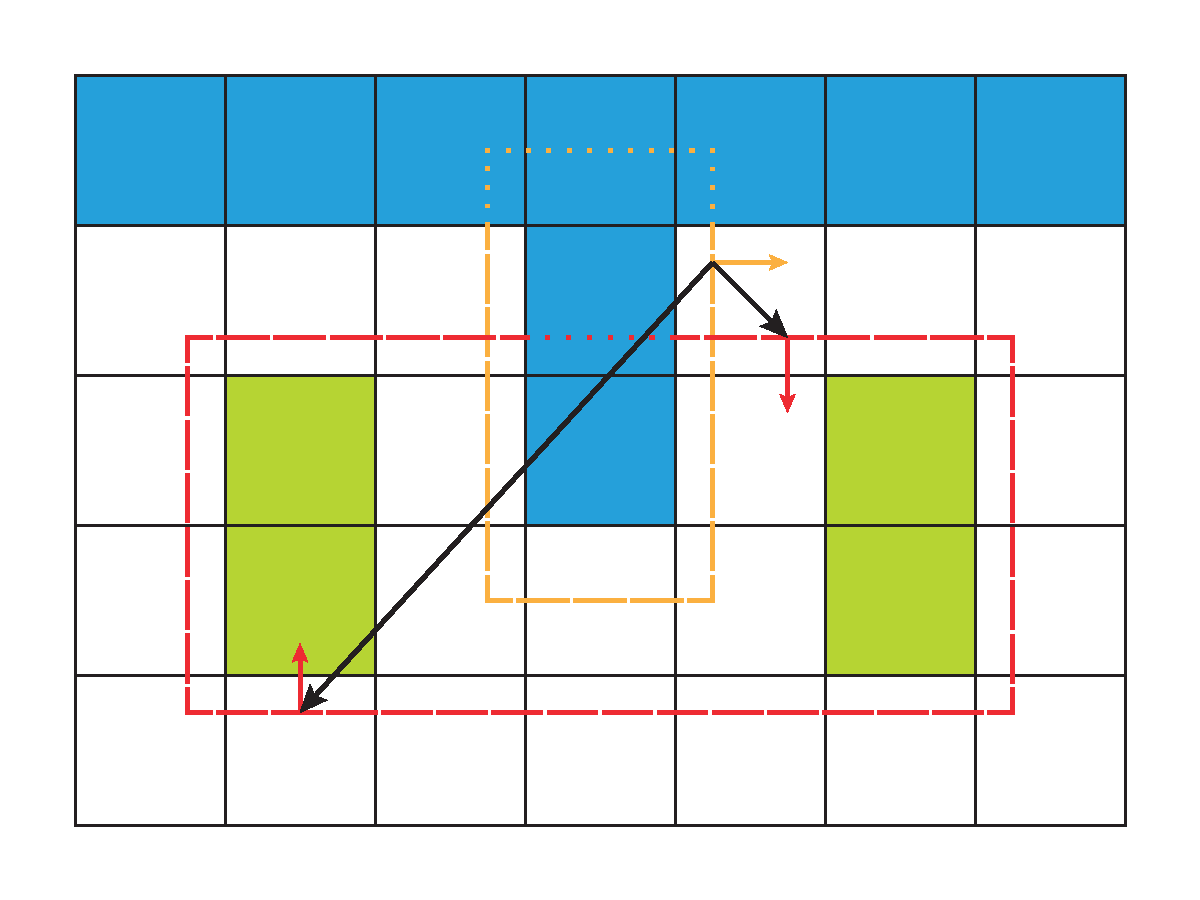
\includegraphics[width=0.8\textwidth]{inside_test_error}
	\caption[Triangle inside structure test]{
		Testing if a triangle of one structure is inside another structure using a ray.
		Due to triangle elimination, the ray can miss removed structures, \eg when traversing outside cells, causing the inside test to fail, \cf left ray.
		As structures are guaranteed to be closed within a cell, this test is only valid within a cell, \cf right ray.
	}
	\label{fig:inside_test_error}
\end{figure}
%
A triangle is tested against a structure by using a ray.
This ray is shot from an arbitrary point on the triangle, which does not lie on an edge, \eg the triangle's centroid, to an arbitrary point on a triangle of the other structure.
If the ray does not intersect the other structure on its way, a comparison of the ray's direction with the normal of the targeted triangle determines whether the ray's origin, \ie the centroid of the tested triangle, is inside the other structure or not.
However, as classification might eliminate triangles, the ray could potentially intersect triangles of the structure which have been removed, \cf left ray in \cref{fig:inside_test_error}.
The regular grid only guarantees closed meshes within a cell.
To circumvent this issue, the inside test for a triangle must be conducted within a cell.

An algorithm for this \textproc{IsTriangleInsideStructure} test is given in \cref{alg:triangle_inside_test}.
%
\begin{algorithm}
	\centering
	\begin{algorithmic}[1]
		\Function{IsTriangleInsideStructure}{$\var{t}, \var{s}$}
			\State $\var{origin} \gets (\var{t}.\var{a} + \var{t}.\var{b} + \var{t}.\var{c}) \div 3$ \Comment{Origin is triangle center}
			\State $\var{target} \gets (\var{s}_0.\var{a} + \var{s}_0.\var{b} + \var{s}_0.\var{c}) \div 3$ \Comment{Target ray at center of $\var{s}_0$}
			\State $\var{ray} \gets \var{target} - \var{origin}$
			\State $\var{d}_{\var{nearest}} \gets \var{ray}.\var{length}()$
			\State $\var{n}_{\var{nearest}} \gets \var{s}_0.\var{normal}$
			\State $\var{raydir} \gets \var{ray}.\var{normalized}()$
			\ForAll{$\var{f} \in \var{s} \setminus \{\var{s}_0\}$} \Comment{Retarget ray at closer triangle if intersected}
				\If{$\Call{IntersectRayTriangle}{\var{origin}, \var{raydir}, \var{f}, \out\var{d}, \out\var{u}, \out\var{v}}$}
					\If{$\var{d} > 0 \wedge \var{d} < \var{d}_{\var{nearest}}$}
						\State $\var{d}_{\var{nearest}} \gets \var{d}$
						\State $\var{n}_{\var{nearest}} \gets \var{f}.\var{normal}$
					\EndIf
				\EndIf
			\EndFor
			\State \Return $\var{n}_{\var{nearest}} \cdot \var{rayDir} \geq 0$
		\EndFunction
		\\
		\Function{IntersectRayTriangle}{$\var{origin}, \var{direction}, \var{t}, \var{d}, \var{u}, \var{v}$}
			\State $\var{vertex}_0 \gets \var{t}.\var{a}$
			\State $\var{edge}_1 \gets \var{t}.\var{b} - \var{t}.\var{a}$
			\State $\var{edge}_2 \gets \var{t}.\var{c} - \var{t}.\var{a}$
			\State $\var{tVec} \gets \var{origin} - \var{vertex}_0$
			\State $\var{pVec} \gets \var{direction} \times \var{edge}_2$
			\State $\var{det} \gets \var{edge}_1 \cdot \var{pVec}$
			\State $\var{u} \gets \var{tVec} \cdot \var{pVec}$
			\State $\var{qVec} \gets \var{tVec} \times \var{edge}_1$
			\State $\var{v} \gets \var{qVec} \cdot \var{direction}$
			\State $\var{invDet} \gets 1 \div \var{det}$
			\State $\var{d} \gets \var{edge}_2 \cdot \var{qVec} \cdot \var{invDet}$
			\State $\var{u} \gets \var{u} \cdot \var{invDet}$
			\State $\var{v} \gets \var{v} \cdot \var{invDet}$
			\State \Return $(\var{u} \geq 0) \wedge (\var{v} \geq 0) \wedge (\var{u} + \var{v} \leq 1)$
		\EndFunction
	\end{algorithmic}
	\caption[Triangle inside structure test]{
		Algorithm for testing whether a triangle is inside another structure.
		The \textproc{IntersectRayTriangle} function is a branch-free version of the famous Möller-Trumbore ray-triangle intersection test \cite{ray_triangle_intersection_moller}.
	}
	\label{alg:triangle_inside_test}
\end{algorithm}
%
The function starts by calculating the origin and target point for the test ray.
The ray originates at the center of the tested triangle and initially targets the center of the first triangle of the other structure.
Distance and normal of the targeted triangle are stored.
Then, all other triangles of the structure are tested for intersection with the created ray.
If an intersection happens and the distance to the newly intersected triangle is shorter than the distance to the currently targeted triangle, the distance and normal are updated to the new triangle, \ie the ray now targets the new triangle.
This procedure ensures that after all triangles have been tested for intersection, the maintained distance and normal store the values of the closest intersection of the ray.
The normal of the closest intersected triangle of the other structure is then finally compared to the ray's direction.
If they point into the same half space, the ray's origin and therefore the tested triangle is inside the tested structure.

For ray-triangle intersection the famous Möller-Trumbore intersection test is used \cite{ray_triangle_intersection_moller}.
An implementation of their algorithm in C is already given in the corresponding work.
The original version has a few early exit tests on \var{u} and \var{v}, which might save some work in case the ray misses the triangle.
However, branching is becoming increasingly expensive on modern hardware architectures, especially in vectorized code paths or GPU code.
A branch-free version of Möller-Trumbore's code, which is currently used and performs slightly better, is shown in \cref{alg:triangle_inside_test}.

The idea of the algorithm is shown in \cref{fig:ray_triangle_intersect}.
%
\begin{figure}
	\centering
	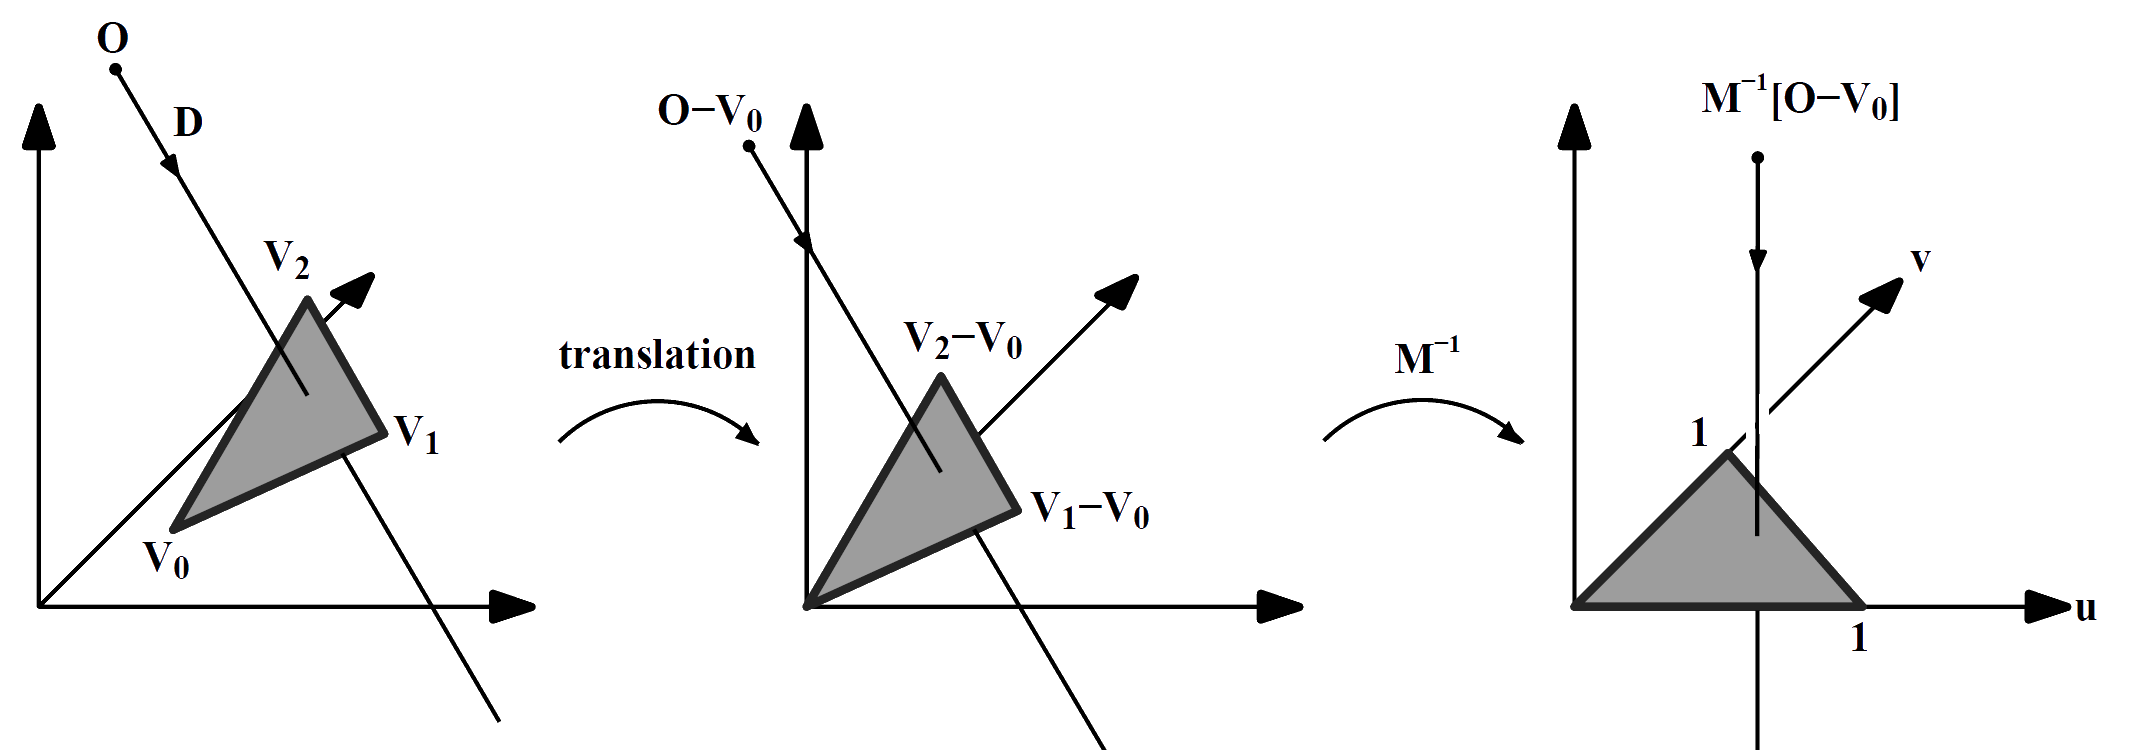
\includegraphics[width=0.9\textwidth]{moeller_trumbore}
	\begin{equation*}
		\left[-D, V_1 - V_0, V_2 - V_0 \right] \left[ \begin{array}{c} t \\ u \\ v \end{array} \right] = O - V_0
	\end{equation*}
	\caption[Möller-Trumbore ray-triangle intersection test]{
		Principle of the famous Möller-Trumbore ray-triangle intersection test \cite{enlight_demo_workshop}.
	}
	\label{fig:ray_triangle_intersect}
\end{figure}
%
The intersection test relies on the idea that, with a simple transformation, the problem can be represented in a coordinate system where the solution is almost given.
This transformation should put the origin of the coordinate system at one vertex of the triangle.
The axes of the new system are the two triangle edges as well as the inverted ray direction.
If the problem is represented in this space, the ray's origin holds the values of the $u$ and $v$ barycentric coordinate of the intersection point on the triangle as well as the distance $t$ of the triangle to the origin in multiples of the ray direction vector's length.
$u$ and $v$ are used to test whether the intersection point lies within the triangle and $t$ can be used as parameter in the line equation of the ray, $X = O + D \cdot t$, to retrieve the point of intersection.
The transformation necessary consists of two steps.
The first is a translation of $O$ by $-V_0$ to move the coordinate system's origin to a triangle vertex.
The second step is a change of basis with $\left[-D, V_1 - V_0, V_2 - V_0 \right]$ as base matrix.
This is done by multiplying with the inverse base matrix.
The result vector $\left[ t,  u,  v \right]$ then contains the desired values.
By moving the multiplication with the inversed base matrix to the other side, the equation in \cref{fig:ray_triangle_intersect} is obtained.
Möller and Trumbore solve this system of equations in matrix form using Cramer's rule.
The determinant of a matrix is calculated using a combination of a cross and a dot product, called the scalar triple product.
This allows to calculate the values of the solution vector incrementally to allow early exits.


\subsection{Numeric improvements}
\label{sec:numeric_improvements}

If the method described in this chapter would be tested on various scenes now, it would barely work for not even modest scenarios.
The problem is mainly numeric instability and the iterative nature of the approach.
Each calculation with a fixed precision is effected by small rounding errors when the result is stored back into a register or to memory.
This especially becomes a problem when theoretically equal calculations should practically yield equal results.
When two incident triangles for example intersect with a third triangle, the shared edge of the first two triangles should intersect at the same point on triangle three.
Depending on the order of operations this is not guaranteed.
The result may be different if, \eg, the two points representing the edge are swapped.
%
The triangle splitting algorithm for example can only hold its guarantees if the intersecting edges are true polylines with no gaps between the segments and their ends are exactly at the triangle edges.
Otherwise, degenerated triangles may be created between intersecting edges or at the triangle edges.
%
Another problem are algorithms which create very small numbers in intermediary calculations.
If a triangle is really thin, the dot product between the edges at the smallest corner is almost zero and suffers from numeric instability.
The cross product and therefore the normal vector also becomes unstable.
Calculations depending on these values might then critically misjudge a situation and \eg create intersection lines outside a triangle or falsely report a triangle as inside-a-structure based on a degenerated normal.
The problem with errors on such hard decisions is that they escalate with the number of iterations, which might be several hundreds or thousands.
If two structures are united but a wrongly discarded triangle left a hole, all following inside tests are affected and may fail.
Several improvements to mitigate degeneration and numeric errors are discussed in this section.

\begin{description}
	% drawings could be added here, but wbackfrieder is OK without

	\item[Collapse near points in structures] \hfill \\
	At the beginning of the \textproc{UnionStructure} algorithm almost no guarantees are given on the two input structures.
	As very thin or degenerated triangles are numerically problematic during the following algorithmic steps, \eg intersection or inside test, filtering them may avoid some of those problems.
	Therefore, all vertices which are closer than a defined small epsilon distance are collapsed to their mean values.
	Thus, no holes are created in the structure, only degenerated triangles.
	These are easy to filter in a post-processing step by removing all triangles where two or more vertices are equal.


	\item[Flush tiny values to zero] \hfill \\
	Floating point values with tiny exponents, \eg $10^{-15}$ and below, tend to make some calculations unstable, especially when collapsing vertices with such coordinates.
	Collapsed vertices with such values might still not compare equal afterwards which breaks subsequent calls to the CDT algorithm.
	The reason therefore is unfortunately not clear.
	However, flushing such small values to zero eliminates the problem.


	\item[Verify intersection line] \hfill \\
	In situations where two triangles are quite thin, the Möller-Trumbore intersection test may report an intersection and calculate an intersection line which lies outside one or both of the triangles.
	Subsequent CDTs will then generate additional triangles outside the split triangle, as CDT routines usually triangulate the convex hull of the input point set.
	This issue is avoided by an additional test run after the call to \textproc{IntersectTriangles}.
	If a triangle intersection is recorded, the points of the intersection line are tested if they lie on each of the triangles.
	The test is performed using a raycast with each point as origin and each triangle normal as ray direction.
	Only if the resulting $u$ and $v$ coordinates for both points are within their bounds including a small epsilon, \ie $-\epsilon \leq u \leq 1+\epsilon \wedge -\epsilon \leq v \leq 1+\epsilon \wedge u + v \leq 1 + \epsilon$, the intersection is accepted.


	\item[Collapse constraint vertices with structure vertices] \hfill \\
	Some of the intersection lines on a triangle might be very close to the triangle's vertices.
	To avoid creating degenerated triangles during CDT, all constraints' vertices are checked against the triangle's vertices to ensure a minimum distance.
	If a distance is less than a specified minimum, the affected vertex is set to the corresponding vertex of the triangle.


	\item[Collapse near points in constraints per triangle] \hfill \\
	This correction is the most important one.
	After all intersection lines have been recorded, collapse all constraint vertices which are closer than a defined epsilon distance.
	This routine ensures that each pair of incident triangles intersecting another triangle produce an incident pair of constraints.
	In other words, constrained edges which are not connected to each other because of numerical issues in the intersection routine are rejoined again to form closed polylines.
	Furthermore, tiny constraints collapse to points and are removed.
	This matter is important for correct splits after running the CDT.


	\item[Ensure unique constraints] \hfill \\
	Constraint uniqueness is a small and simple check.
	The test is required as duplicated constraints impose a problem for some CDT libraries.


	\item[Specify hull constraints] \hfill \\
	Most CDT libraries triangulate a given point cloud within the convex hull of the cloud.
	Identifying the edges belonging to the convex hull is usually deterministic if the points are in what is called general position, \ie no coincident or collinear points.
	However, the vertices of a triangle and a set of constraints where many constraints end at the triangle's edges contain a lot of collinear points.
	In order to help the CDT in finding the right hull, it is recommended to specify the hull manually via additional constraints.
	These hull constraints are constructed from the triangle's vertices and the constraint vertices touching an edge of the triangle.
	The latter are identified by counting the number of constraints incident to each vertex of a point set formed by all constraints' vertices.
	Vertices with only one incident constraint must lie at the triangle's border and are therefore hull vertices.
	Together with the triangle's vertices, the hull vertices are ordered cyclical around their center of mass.
	The hull constraints are then formed from each adjacent pair of the ordered hull vertices including the constraint from the last to the first hull vertex.
	These hull constraints are appended to the constraints created by the intersection lines as input to the CDT.


	\item[Remove degenerate triangles after CDT] \hfill \\
	Despite good preparation of the input, it might still be the case that tiny or degenerated triangles are generated by the CDT routine, especially along the hull.
	The vertices of such triangles are apart far enough to pass vertex collapse in a following iteration.
	Therefore, a check on the triangle's angles is preferred.
	If the dot product of any pair of incident, normalized edges of the triangle is approaching zero, \ie is below a defined epsilon, the triangle is removed from the triangulation result.
\end{description}


\subsection{Parallelization}
\label{sec:parallelization}

By choosing to solve the intersections of all structures per cell, the main routine in \cref{alg:direct_intersection} became embarrassingly parallel.
As the regular grid usually consists of a larger number of cells, \eg $100 \times 100 \times 100$ is quite common, scheduling each cell in parallel is probably the best option for parallelization.
However, a good scheduling strategy is needed, as the workload per cell is highly diverse.
Most of the cells are empty because they are either inside or outside cells and require no processing.
But also the amount of triangles and structures in each surface cell varies drastically between a few triangles and several thousands.

If all structures would be closed, \ie triangle elimination by classification would be disabled, and there would be no subdivision into cells, the iterative creation of the union structure could be parallelized instead.
Always combining two elements of a set of elements until only one is left is an algorithm known as reduction, fold or accumulation.
Reductions are usually parallelized as a tree.
Each independent pair of elements can be reduced into one in parallel.
However, tree-shaped parallel reduction offers suboptimal parallelism, especially against the end where only a few parallel pairs remain.
Parallelizing the reduction of all surfaces into one, in addition to a cell-based parallelization, is probably superfluous.
The still high number of surface cells provide enough parallel work to saturate most workstations or even server CPUs.

Most routines inside the \textproc{UnionStructure} algorithm are also viable candidates for parallelization, although the workload is significantly smaller.
A structure inside a cell usually does not consist of more than 50 - 100 triangles.
These routines would probably benefit from data parallelism and SIMD constructs, \ie vectorization.
Especially the \textproc{ClipPolygonAABB}, \textproc{IntersectTriangles} and \textproc{IsTriangleInsideStructure} algorithms contain only a few branches and operate on simple data structures, \ie arrays.

Considering alternative hardware architectures like GPUs or similar accelerators, \eg Intel's Xeon Phi coprocessor, a parallelization based on the regular grid's cells is recommended.
The reason is that the number of cells is known at the beginning of the whole calculation which allows static scheduling of the entire work size.
This property is mandatory when programming for GPUs, but has been softened in recent years by the introduction of dynamic parallelism in CUDA 5.0 and OpenCL 2.0.
Furthermore, most GPU architectures rely on either vectorization or execution of thread groups in lockstep\footnote{
	Most GPUs usually schedule groups of threads, called warps with 32 threads by NVIDA and wavefronts with 64 threads by AMD.
	These threads are tied together and executed instruction-wise, meaning all threads execute the same instruction on their individual data in parallel.
	This behavior is also called lockstep execution and the paradigm single instruction, multiple threads (SIMT).
	If some threads branch differently than others, \eg if, while or for statements, all threads execute both branches, but some of them are masked out to avoid changes by the executed instructions.
	Intel's on-chip GPUs rely on vectorization which has to be done manually by the programmer for medium and advanced algorithms.} to achieve a high throughput.
Thus, the uneven workloads in all loops, \eg number of structures per cell, number of triangles per structure or number of intersections, hardly saturate these architectures, probably causing many threads to run empty loops because of a few larger cells or structures.

In the underlying implementation, only the topmost loop of the \textproc{DirectIntersection} function has been parallelized using Microsoft's Parallel Patterns Library (PPL) and the parallel\_for function which uses a scheduler implementing work stealing to balance the workload \cite{ppl_parallel_for}.


\chapter{Method 2: Tri-dexel}
\label{ch:tri_dexel}

The second discussed method to extract a triangulated surface from the VML's data model is based on a tri-dexel representation, \cf section \ref{sec:surface_representations}.
As observed with the previously shown method in chapter \ref{ch:direct_intersection}, reconstructing a surface directly form the many intersecting triangles stored in the VML's grid is computationally expensive, highly numerically unstable and prone to errors.
A more robust approach is desirable, which is able to always successfully reconstruct a surface with good quality.
This reconstruction should succeed independently of the complexity of the maintained geometry.
As a trade-off for this robustness, the approach may sacrifice surface exactness and filigree features.
Dexel-based representations fit this purpose nicely.
They provide a good abstraction of a machined workpiece with rich semantics.
The used grid resolution supplies an easy to configure level of detail and steering parameter between representation quality and memory/CPU demands.
Creating dexel-based representations from the VML's data model is achieved using an adaption of the already implemented, well-working and robust raycasting subsystem used for visualization, \cf section \ref{sec:raycasting}.
To achieve a good portrayal independently of the workpiece's orientation, three axis-aligned dexel images will be generated, thus creating a tri-dexel representation.
For converting such a tri-dexel model into a final triangle mesh, various algorithms are found in literature.
An excellent example is Ren \etal's "Feature Conservation and Conversion of Tri-dexel Volumetric Models to Polyhedral Surface Models for Product Prototyping" \cite{tridexel_reconstruction}.
Their approach form the idea and foundation of the implementation presented in this chapter.


\section{Concept}
\label{sec:tri_dexel_concept}

Firstly, a tri-dexel representation of the VML's data model has to be obtained.
Dexel images, in general, are created by sampling the workpiece's surface along parallel lines.
This sampling process is already implemented in the raycasting subsystem as part of the visualization.
However, when sampling dexels, a ray must not stop at the first surface intersection, but continue through the whole data model and collect all intersections along its path.
At each intersection, the intersection depth, \ie distance from the ray's origin, and the surface normal of the intersected triangle is recorded as a dexel node.
From the dexel's origin and a node's depth the intersection point can be calculated.
The raycast itself is performed with axis-parallel rays starting at equidistant origins from three sides of the VML's data model, thus creating three dexel images.
Combining these dexel images creates a uniform regular grid, the tri-dexel grid.
Figure \ref{fig:cylinder_head_dexel} shows the cylinder head scene with a low-resolution dexel image and the final reconstruction.

\begin{figure}
	\centering
	\begin{subfigure}[t]{0.3\textwidth}
		\centering
		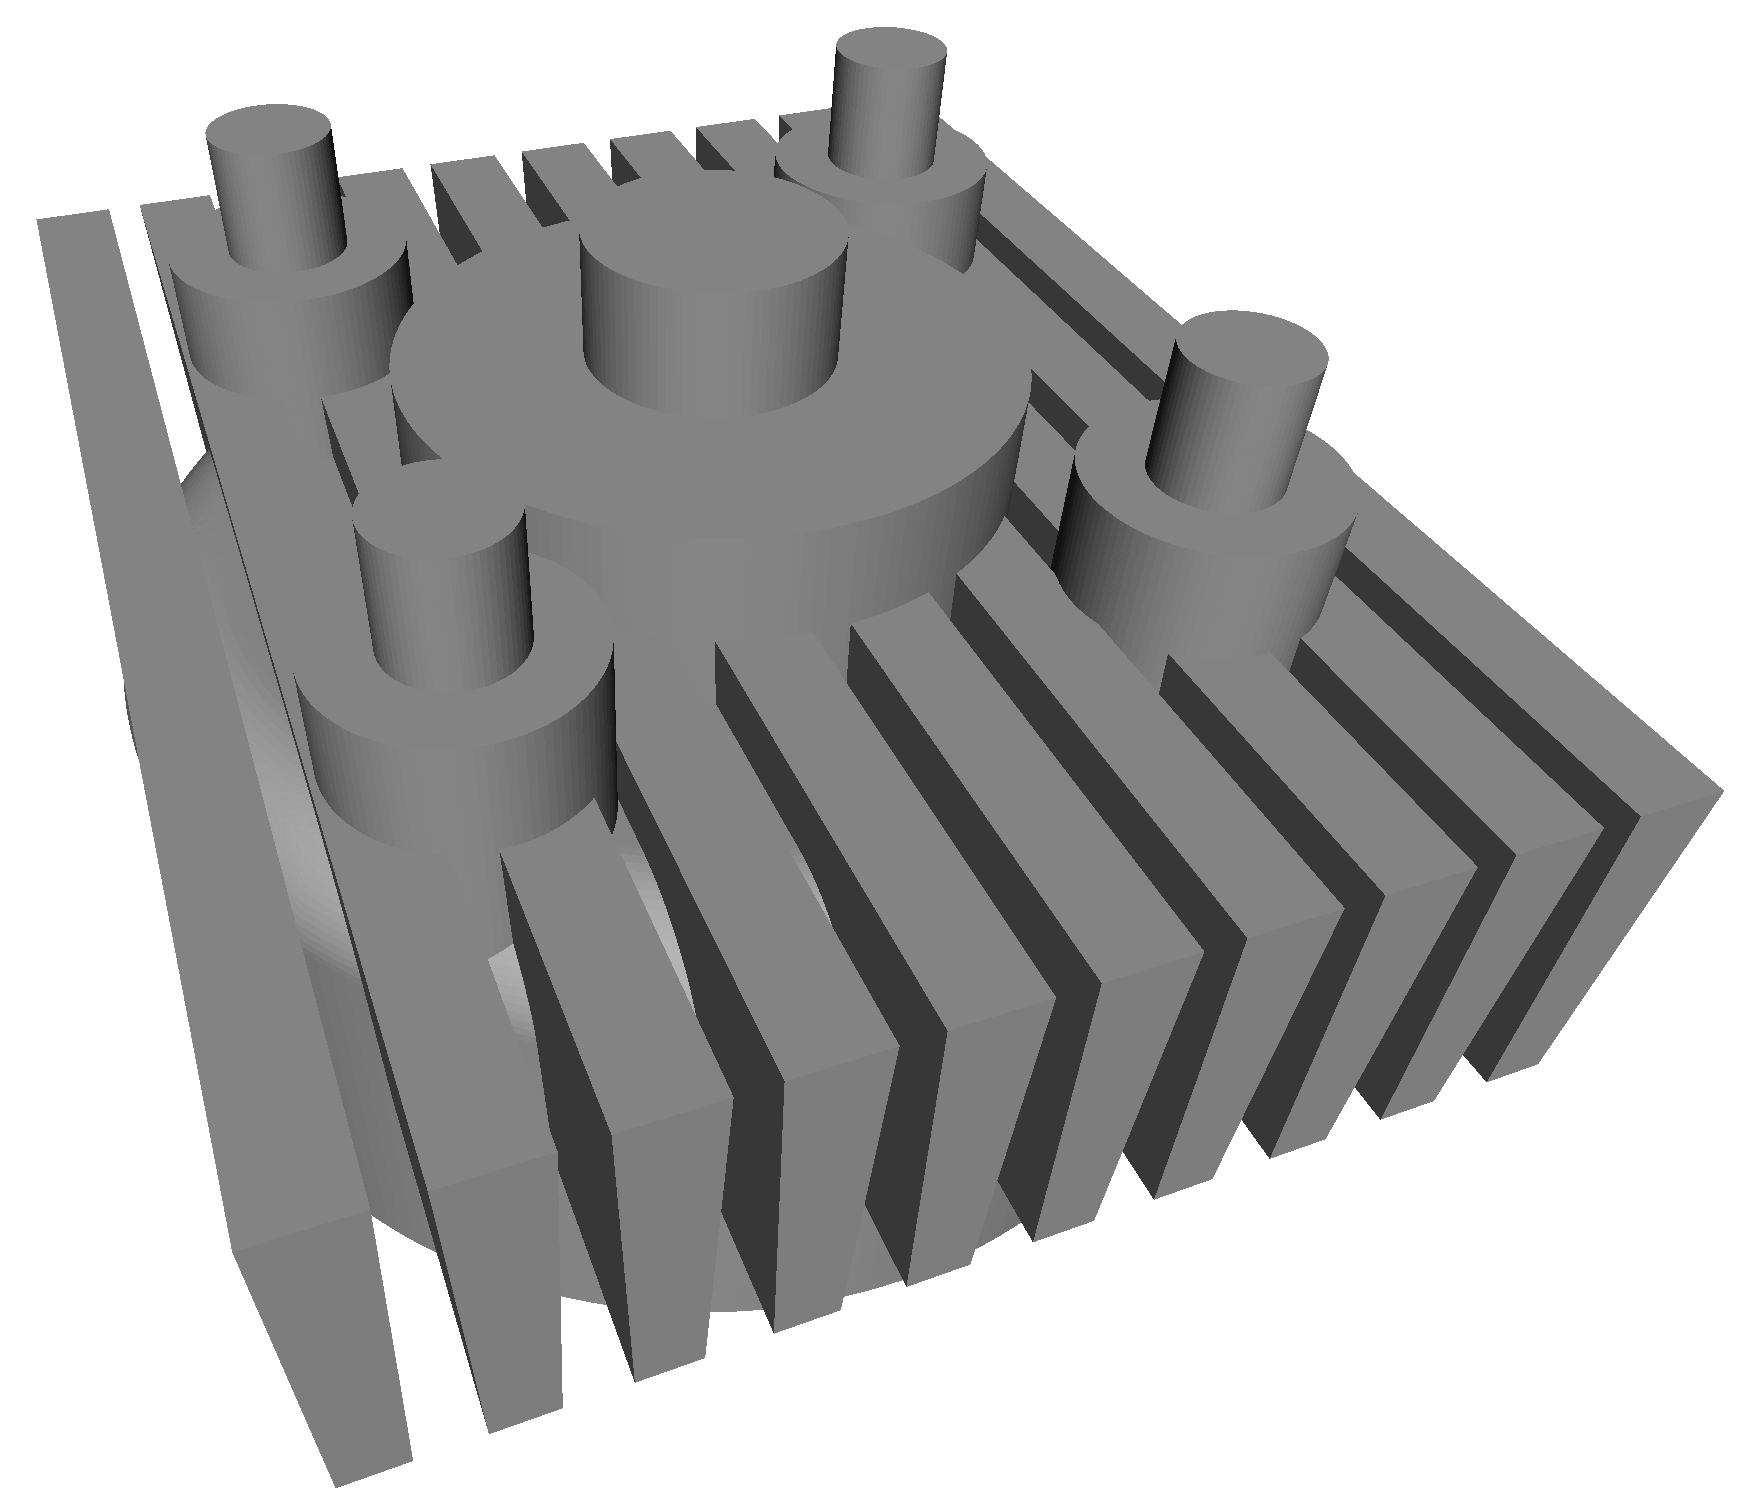
\includegraphics[width=\textwidth]{images/cylinder_head_stock_and_svs}
		\caption{Stock and SVs}
		\label{fig:cylinder_head_stock_sv}
	\end{subfigure}
	\begin{subfigure}[t]{0.3\textwidth}
		\centering
		\includegraphics[width=\textwidth]{images/cylinder_head_vml}
		\caption{VML}
		\label{fig:cylinder_head_classified}
	\end{subfigure}
	\begin{subfigure}[t]{0.3\textwidth}
		\centering
		\includegraphics[width=\textwidth]{images/cylinder_head_dexel_image}
		\caption{Tri-dexel image}
		\label{fig:cylinder_head_dexel_image}
	\end{subfigure}
	\begin{subfigure}[t]{0.3\textwidth}
		\centering
		\includegraphics[width=\textwidth]{images/cylinder_head_dexel_image_center}
		\caption{Tri-dexel image center}
		\label{fig:cylinder_head_dexel_image_center}
	\end{subfigure}
	\begin{subfigure}[t]{0.3\textwidth}
		\centering
		\includegraphics[width=\textwidth]{images/cylinder_head_dexel_image_fins}
		\caption{Tri-dexel image fins}
		\label{fig:cylinder_head_dexel_image_fins}
	\end{subfigure}
	\begin{subfigure}[t]{0.3\textwidth}
		\centering
		\includegraphics[width=\textwidth]{images/cylinder_head_reconstructed}
		\caption{Result}
		\label{fig:cylinder_head_reconstructed}
	\end{subfigure}
	\caption{
		Tri-dexel based surface reconstruction from the VML's data model of a cylinder head.
		Figure \ref{fig:cylinder_head_stock_sv} shows the stock and a few swept volumes creating the fins and drillings.
		Figure \ref{fig:cylinder_head_classified} shows the classification result after these solids have been mapped into the VML's regular grid.
		The removed triangles are clearly visible, especially at the swept volumes.
		By using a raycast of axis parallel rays along all three coordinate system axes a tri-dexel representation is created as shown in figure \ref{fig:cylinder_head_dexel_image}.
		The resolution of the grid spawning the rays is 30 along the longest dimension.
		Figure \ref{fig:cylinder_head_dexel_image_center} and \ref{fig:cylinder_head_dexel_image_fins} show details of the tri-dexel image.
		The former views the drilling at the center from above and the latter views the cylinder head's fins from the center.
		Finally, the reconstructed surface is shown in figure \ref{fig:cylinder_head_reconstructed}.
		Note the imperfections at the fin's edges and bases.
	}
	\label{fig:cylinder_head_dexel}
\end{figure}

Secondly, the tri-dexel representation is converted into a triangle mesh.
This procedure is mostly based on the paper already mentioned during the introduction \cite{tridexel_reconstruction}.
Each intersection point of three orthogonal dexels from the tri-dexel grid forms a grid point.
If a grid point lies within a dexel segment on any of these dexels, it is said to be occupied, \ie lies within the workpiece's volume.
8 grid points and their 12 connecting edges along with their dexel segments are grouped into cells of the grid.
Each grid cell is then processed independently.
Figure \ref{fig:tri_dexel_cell} shows the structure of a tri-dexel cell.
%
\begin{figure}
	\centering
	\includegraphics[width=0.5\textwidth]{images/tri_dexel_cell}
	\caption{
		A cell of a tri-dexel grid \cite{tridexel_reconstruction}.
		Occupied grid points are drawn in red, dexel nodes in green, dexel segments in blue.
		Each grid point is referenced using a number between 0 and 7 and has a list of neighboring grid points in counter-clockwise order, \cf left table.
	}
	\label{fig:tri_dexel_cell}
\end{figure}
%
Before a cell can be triangulated, a few consistency checks and corrections are applied to the cell.
This process is called regularization and ensures a successful triangulation into a water-tight mesh.
After ensuring the consistency of a cell, it can be triangulated.
For this purpose, a depth-first search process is iteratively started at non-occupied grid points of the cell to discover boundary loops.
Basically, the found loops can be triangulated right away to obtain a water tight mesh.
However, the quality of the triangulation can be further enhanced by taking normal information at the dexel nodes into account.
This is especially necessary to reconstruct features of the model.
This optional feature reconstruction pass is run on the loops found in the previous step and may create additional vertices.

\section{Implementation}
\label{sec:tri_dexel_implementation}

In order to run the tri-dexel surface reconstruction, the user must supply a resolution as parameter.
This resolution determines the size of the raycasted dexel images as well as the resulting tri-dexel grid.
For esthetic reasons, the specified resolution is only used for the longest dimension of the workpiece.
The resolution along the other dimensions is usually smaller in order to make the cells more cubic, although the implementation does not require cubic cells.


In addition to the types already specified by the VML, \cf figure \ref{fig:vml_datamodel}, the tri-dexel reconstruction algorithm requires a few more types.
Most of these type definitions and also the algorithms themselves are vastly simplified when compared with the underlying source code.
Especially parallelism, asynchrony, memory efficient handling of data structures and numeric stability enhancements have been intentionally left out in the discussed pseudo code.
The additional types needed for the tri-dexel implementation are shown in the class diagram in figure \ref{fig:tri_dexel_datamodel}.
%
\begin{figure}
	\centering
	\includegraphics[width=0.9\textwidth]{images/tri_dexel_datamodel}
	\caption{
		Simplified UML class diagram of the types needed for the tri-dexel reconstruction algorithm in addition to the types used by the VML, \cf figure \ref{fig:vml_datamodel}.
	}
	\label{fig:tri_dexel_datamodel}
\end{figure}
%
The most central data structure is the \var{TriDexelGrid} class.
It represents a tri-dexel representation of the complete VML workpiece which is already prepared for subsequent regularization and triangulation.
In addition to the tri-dexel grid's resolution \var{res} and bounding box \var{aabb}, the \var{TriDexelGrid} class further contains the occupancy information for each grid point in \var{occupancy}, \ie whether a grid point is spanned by a dexel or not, as well as the actual dexel segments between the grid points, stored in \var{edges}.
The \var{cells} method separates all this information into distinct and independent cells.
Each cell is an instance of the \var{Cell} class and contains the same information as the tri-dexel grid, but locally for a single cell.
A cell stores it's bounding box \var{box}, the point occupancy of each of the cell's corners in \var{occupancy}, the corners' coordinates in \var{realPoints} and the 12 edges of the cell, stored in \var{edges}.
Each edge of the cell is an instance of \var{Edge} and contains all spanning dexel segments, clamped to the interval between the edge's incident grid points.
Furthermore, a method \var{isBoundary} is provided to check if the cell is a boundary cell, \ie contains occupied and non-occupied grid points and therefore contains a part of the workpiece's surface.
The \var{TriDexelGrid} is constructed from the \var{TriDexelImage} class, which, fundamentally, contains the same information as the tri-dexel grid.
The difference is substantially clearer from the workflow's point of view.
Whereas the \var{TriDexelGrid} is already prepared for further processing, the \var{TriDexelImage} class only contains the raw result as created by raycasting the VML's data model from three orthogonal directions.
This data only consists of the resolution \var{res} used for raycasting as well as three dexel images \var{images} along the three coordinate system axes.
A \var{DexelImage} describes the result of a single raycast along the axis specified in \var{axis0}, where 0 denotes the x-, 1 the y- and 2 the z-axis.
The members \var{axis1Res} and \var{axis2Res} store the resolution of the dexel image along the two cyclically following axes after \var{axis0}.
For example, if \var{axis0} is 1, the y-axis, then \var{axis1Res} and \var{axis2Res} hold the resolutions along the axes 2 and 0, the z- and x-axis.
Finally, \var{dexels} contains all the dexels of the image.
Each \var{Dexel} instance is then essentially a list of nodes, stored in \var{nodes}.
The number of stored nodes after raycasting is always a multiple of two.
As dexel nodes are typically processed in pairs, as dexel segments, a convenience method \var{segments} is provided which groups adjacent nodes into instances of \var{DexelSegment}.
A \var{DexelSegment} contains these two nodes as \var{start} and \var{end} node.
Finally, the \var{Node} class holds the depth of the node along its dexel, \ie the distance of the node from the plane where the dexels originate, \cf figure \ref{fig:dexel_image}, as well as the normal vector of this surface entry/exit.
Unrelated to the tri-dexel types is the additional class \var{Ray} which represents a ray starting at the vertex \var{origin} and traveling into the direction stored by \var{direction}.

Based on the discussed tri-dexel types, the basic reconstruction algorithm is shown in algorithm \ref{alg:tri_dexel}.
%
\begin{algorithm}
	\centering
	\begin{algorithmic}[1]
		\Function{TriDexel}{$\var{grid}, \var{resolution}$}
			\State $\var{box} = \var{Extends}(\var{grid}.\var{aabb}.\var{lower} - \epsilon, \var{grid}.\var{aabb}.\var{upper} + \epsilon)$
			\State $\var{res} = \Call{UniformResolution}{\var{box}, \var{resolution}}$
			\State $\var{img} = \var{TriDexelImage}(\var{res})$
			\State $\Call{AxisParallelRaycast}{\var{grid}, \var{box}, \var{res},\hfill\break
				\hspace*{\dimexpr\algorithmicindent*2}(\var{axis}, \var{x}, \var{y}, \var{v}, \var{n}) \rightarrow \var{img}.\var{images}_{\var{axis}}.\var{dexels}_{\var{x}, \var{y}}.\var{nodes}.\var{add}(\var{Node}(\var{v}_{\var{axis}}, \var{n}))}$
			\State $\var{dgrid} = \Call{CreateTriDexelGrid}{\var{img}, \var{box}}$
			\State $\var{triangles} \gets \varnothing$
			\ForAll{$\var{c} \in \var{dgrid}.\var{cells}()$}
				\State $\Call{RegularizeCell}{\var{c}}$
				\State $\var{triangles} \gets \var{triangles} \cup \Call{TriangulateCell}{\var{c}}$
			\EndFor
			\State \Return $\var{triangles}$
		\EndFunction
	\end{algorithmic}
	\caption{
		Abstract workflow of the surface reconstruction using a tri-dexel approach.
	}
	\label{alg:tri_dexel}
\end{algorithm}
%
At the beginning, a slightly enlarged bounding box is calculated for the size of the tri-dexel grid and raycast.
In this way, edge cases with a surface exactly at the grid's border are avoided.
The \textproc{UniformResolution} function takes the user-specified resolution and the tri-dexel grid's bounding box and calculates three resolutions, one for each axis.
The longest one is equal to the specified resolution and the other two are calculated in such a way that the resulting cells of the tri-dexel grid are as cubic as possible.
This resolution is used to preallocate space for the tri-dexel image which is then filled in the subsequent raycasting process.
The remaining part of the algorithm closely follows the concept discussed in the previous section\ref{sec:tri_dexel_concept}.
The subsequent sections discuss the functions and procedures of the algorithm in the order they are used.


\subsection{Raycast}
\label{sec:tri_dexel_raycast}

The raycast is the prime algorithm for converting the VML's data model into a tri-dexel representation.
The raycast is performed with parallel, axis-aligned and equidistant rays.
All rays start at the intersection points of a uniform 2-dimensional grid placed on one side of the data model's slightly enlarged bounding box and end at the opposite side, \cf figure \ref{fig:dexel_image}.
Three of these raycasts along the three axes of the coordinate system result in three dexel images.
As the raycasting code is kept separated from the tri-dexel data structures, a function is passed to the raycasting code which is invoked each time a ray has found a surface intersection.
Therefore, the same code can be used to create other data structures as well. %TODO: ref point cloud creation

The entry routine and ray creation code of the raycasting algorithm is shown in algorithm \ref{alg:tri_dexel_raycast}.
%
\begin{algorithm}
	\centering
	\begin{algorithmic}[1]
		\Procedure{Raycast}{$\var{grid}, \var{box}, \var{res}, \var{hitFunc}$}
			\For{$\var{axis0} \gets 0 \To 2$}
				\State $\var{axis1} \gets (\var{axis0} + 1) \bmod 3$
				\State $\var{axis2} \gets (\var{axis0} + 2) \bmod 3$
				\State $\var{xCount} \gets \var{res}_{\var{axis1}}$
				\State $\var{yCount} \gets \var{res}_{\var{axis2}}$
				\State $\Delta \var{x} \gets (\var{box}.\var{upper}_{\var{axis1}} - \var{box}.\var{lower}_{\var{axis1}}) \div (\var{xCount} - 1)$
				\State $\Delta \var{y} \gets (\var{box}.\var{upper}_{\var{axis2}} - \var{box}.\var{lower}_{\var{axis2}}) \div (\var{yCount} - 1)$
				\For{$\var{y} \gets 0 \To \var{yCount} - 1$}
					\For{$\var{x} \gets 0 \To \var{xCount} - 1$}
						\State $ray = \Call{CreateRay}{\var{box}, \var{axis0}, \var{axis1}, \var{axis2}, \var{\Delta x}, \var{\Delta y}, \var{x}, \var{y}}$
						\State $\Call{CastRay}{\var{grid}, \var{axis0}, \var{axis1}, \var{axis2}, \var{ray},\hfill\break
							\hspace*{\dimexpr\algorithmicindent*5}(\var{v}, \var{n}) \rightarrow \var{hitFunc}(\var{axis0}, \var{x}, \var{y}, \var{v}, \var{n})}$
					\EndFor
				\EndFor
			\EndFor
		\EndProcedure
		\\
		\Function{CreateRay}{$\var{box}, \var{axis0}, \var{axis1}, \var{axis2}, \var{\Delta x}, \var{\Delta y}, \var{x}, \var{y}, \var{xCount}, \var{yCount}$}
			\State $\var{origin} \gets \var{box}.\var{lower}$
			\State $\var{origin}_{axis1} \gets \var{origin}_{\var{axis1}} + \var{x} * \var{\Delta x}$
			\State $\var{origin}_{axis2} \gets \var{origin}_{\var{axis2}} + \var{y} * \var{\Delta y}$
			\State $\var{direction} = \var{Vertex}(0, 0, 0)$
			\State $\var{direction}_{\var{axis0}} \gets 1$
			\State \Return $\var{Ray}(\var{origin}, \var{direction})$
		\EndFunction
		\\
		\Procedure{CastRay}{$\var{grid}, \var{axis0}, \var{axis1}, \var{axis2}, \var{ray}, \var{hitFunc}$}
			\State $\var{traverser} \gets \var{AxisAlignedTraverser}(\var{grid}, \var{ray}, \var{axis0}, \var{axis1}, \var{axis2})$
			\While{$\neg \var{traverser}.\var{reachedEnd}()$}
				\State $\var{cell} \gets \var{traverser}.\var{nextCell}()$
				\State $\Call{IntersectCell}{\var{cell}, \var{ray}, \var{axis0}, \var{axis1}, \var{axis2}, \var{hitFunc}}$
			\EndWhile
		\EndProcedure
	\end{algorithmic}
	\caption{
		Basic algorithm for performing a parallel raycast along all three coordinate system axes on the VML's data model.
	}
	\label{alg:tri_dexel_raycast}
\end{algorithm}
%
The outmost procedure \textproc{Raycast} takes four arguments: the VML's regular grid data structure, the slightly enlarged bounding box of the raycasted area, the resolution of the raycasted \enquote{image} as well as a function, which is called on every surface hit.
The algorithm starts of by iterating over the three coordinate system's axes.
The index of each axis is stored in the variable \var{axis0}, where 0 denotes the x-, 1 the y- and 2 the z-axis.
\var{axis0} is also called primary axis and is accompanied by \var{axis1} and \var{axis2} which hold the other two, secondary axes, in cyclic order.
Depending on the choice of primary and secondary axes, the resolution of the 2-dimensional grid spawning the rays is determined and assigned to \var{xCount} and \var{yCount}, for the horizontal and vertical resolution.
Afterwards, the distance between two incident rays along both secondary axes is computed.
Therefore, along both secondary axes, the size of the bounding box is computed and divided by the resolution minus one.
The result is assigned to the variables \var{\Delta x} and \var{\Delta y}.
Now the algorithm starts creating and casting all rays along their primary axis.
Two nested loops iterate over all points of the 2-dimensional grid spawning rays.
For each grid point at $\var{x}, \var{y}$ a ray is created using the \textproc{CreateRay} function.
Subsequently, the ray is cast into the VML's regular grid by invoking \textproc{CastRay}, passing a closure which is invoked each time a hit is recorded.

The \textproc{CreateRay} function's objective is to create an instance of \var{Ray} storing the ray's origin and direction.
The origin is calculated by starting from the bounding box's \var{lower} corner.
Along the primary axis, this value is already correct.
On the secondary axes, the origin, currently at the origin for ray $0, 0$, must be moved according to the ray's \var{x} and \var{y} coordinate.
In order to do so, \var{x} and \var{y} are multiplied by the distances between incident rays, \var{\Delta x} and \var{\Delta y}, and added to the origin's secondary axes.
%
Computing the ray's direction is simpler, as it is axis aligned.
Therefore, the direction is a unit vector along the primary axis, created by setting the corresponding component of a zeroed vector to one.
%
Finally, \var{origin} and \var{direction} are aggregated into an instance of \var{Ray} and returned.

After rays have been created, they are cast into the VML's regular grid data structure to find surface intersections using the \textproc{CastRay} procedure.
Traversing a ray through a regular grid is usually done using the 3D-DDA algorithm \cite{3DDDA}, \cf figure \ref{fig:traverser}.
However, as the rays are axis parallel, traversal essentially boils down to mapping the ray's origin to the appropriate grid cell and incrementing the 3-dimensional cell index along the primary axis until the other end of the grid is reached.
This logic is hidden behind the \var{AxisAlignedTraverser} class and is no further elaborated.
%
The ray is then intersected with each cell pulled from the traverser using the \textproc{IntersectCell} algorithm.
Fundamentally, the implementation is based on the inside counting scheme of the visualization code explained in figure \ref{fig:raycast}.
The important difference is that the raycast for visualization may terminate after the first intersection found.
Furthermore, minor inconsistencies are tolerable and may result in a few pixel errors on the final image.
However, when creating dexels, a consistent number of surface entries and exits as well as numerically correct ordering of the intersections is substantial.
Consequently, such an intersection routine must employ a great deal of numeric precautions and extra checks to deliver a correct result, even sacrificing intersections for the sake of consistency.
This procedure forms the heart of the raycasting algorithm.
As it is quite comprehensive and highly tailored to the VML's internal data structures, the detailed pseudocode of the \textproc{IntersectCell} routine is omitted from the thesis.


\subsection{Tri-dexel image and grid generation}
\label{sec:tri_dexel_dexel_image_generation}

Based on the generic, axis parallel raycasting routine, a tri-dexel image is created in the base algorithm \ref{alg:tri_dexel}.
Before the raycast is lauched, an instance of \var{TriDexelImage} is created, preallocating enough space to hold 3 dexel images, each holding a 2-dimensional grid of empty dexels.
When calling \textproc{AxisParallelRaycast} procedure, an anonymous function is passed which is invoked on every surface hit detected during raycasting.
This function receives the primary axis \var{axis}, \ie the axis along the rays where traversed, \var{x} and \var{y} coordinate on the 2-dimensional dexel grid as well as the intersection point \var{v} with the normal of the hit triangle \var{n}.
With this information, the tri-dexel image stored in \var{img} is populated.
Once raycasting has completed, the tri-dexel grid is generated from the tri-dexel image.
This conversion is more a reinterpretation and preparation of the information contained within the tri-dexel image.
Whereas the image contains the raw raycasting result, the tri-dexel grid already stores grid point occupancy information and cuts all dexels at cell borders.
This preparation eases the follow-up processing of individual cells.

Converting the tri-dexel image into a tri-dexel grid is done by the \textproc{CreateTriDexelGrid} function, which is shown in algorithm \ref{alg:tri_dexel_grid_generation}.
%
\begin{algorithm}
	\centering
	\begin{algorithmic}[1]
		\Function{CreateTriDexelGrid}{$\var{triImg}, \var{box}$}
			\State $\var{res} = \var{triImg}.\var{res}()$
			\State $\var{grid} = \var{TriDexelGrid}(\var{res}, \var{box})$
			\For{$\var{axis0} \gets 0 \To 2$}
				\State $\var{axis1} \gets (\var{axis0} + 1) \bmod 3$
				\State $\var{axis2} \gets (\var{axis0} + 2) \bmod 3$
				\For{$\var{axis1Val} \gets 0 \To \var{res}_{\var{axis1}} - 1$}
					\For{$\var{axis2Val} \gets 0 \To \var{res}_{\var{axis2}} - 1$}
						\State $\var{dexel} \gets \var{triImg.images}_{\var{axis0}}.\var{dexels}_{\var{axis1Val}, \var{axis2Val}}$
						\ForAll{$\var{seg} \in \var{dexel}.\var{segments}()$}
							\LineComment{Compute affected grid point range}
							\State $\var{start} \gets \floor{\Call{MapDepthToGrid}{\var{seg}.\var{start}.\var{depth}, \var{axis0}, \var{res}, \var{box}}}$
							\State $\var{end} \gets \floor{\Call{MapDepthToGrid}{\var{seg}.\var{end}.\var{depth}, \var{axis0}, \var{res}, \var{box}}}$
							\For{$\var{axis0Val} \gets \var{start} \To \var{end}$}
								\State $\var{gridFrom}$
								\State $\var{gridFrom}_{\var{axis0}} \gets \var{axis0Val}$
								\State $\var{gridFrom}_{\var{axis1}} \gets \var{axis1Val}$
								\State $\var{gridFrom}_{\var{axis2}} \gets \var{axis2Val}$
								\State $\var{gridTo} \gets \var{gridFrom}$
								\State $\var{gridTo}_{axis0} \gets \var{gridTo}_{\var{axis0}} + 1$
								\State $\var{depthFrom} = \Call{MapGridToDepth}{\var{gridFrom}_{\var{axis0}}, \var{axis0}, \var{res}, \var{box}}$
								\State $\var{depthTo}   = \Call{MapGridToDepth}{\var{gridTo}_{\var{axis0}}, \var{axis0}, \var{res}, \var{box}}$
								\LineComment{Point occupancy}
								\If{$\var{seg}.\var{start}.\var{depth} \leq \var{depthFrom} \leq \var{seg}.\var{end}.\var{depth}$}
									\State $\var{grid}.\var{occupancy}_{\var{gridFrom}} \gets \True$
								\EndIf
								\If{$\var{seg}.\var{start}.\var{depth} \leq \var{depthTo} \leq \var{seg}.\var{end}.\var{depth}$}
									\State $\var{grid}.\var{occupancy}_{\var{gridTo}} \gets \True$
								\EndIf
								\LineComment{Copy and clamp to cell border}
								\State $\var{s} \gets \var{seg}$
								\If{$\var{s}.\var{start}.\var{depth} \leq \var{depthFrom}$}
									\State $\var{s}.\var{start}.\var{depth} \gets \var{depthFrom}$
								\EndIf
								\If{$\var{s}.\var{end}.\var{depth} \geq \var{depthTo}$}
									\State $\var{s}.\var{end}.\var{depth} \gets \var{depthTo}$
								\EndIf
								\State $\var{grid}.\var{edges}_{\var{axis0}, \var{gridFrom}}.\var{segments}.\var{add}(\var{s})$
							\EndFor
						\EndFor
					\EndFor
				\EndFor
			\EndFor
		\EndFunction
		\Function{MapDepthToGrid}{\var{depth}, \var{axis0}, \var{res}, \var{box}}
			\State \Return $(\var{depth} - \var{box}.\var{lower}_{\var{axis0}}) \div (\var{box}.\var{upper}_{\var{axis0}} - \var{box}.\var{lower}_{\var{axis0}}) * (\var{res}_{\var{axis0}} - 1)$
		\EndFunction
		\Function{MapGridToDepth}{\var{gridCoord}, \var{axis0}, \var{res}, \var{box}}
			\State \Return $\var{gridCoord} \div (\var{res}_{\var{axis0}} - 1) * (\var{box}.\var{upper}_{\var{axis0}} - \var{box}.\var{lower}_{\var{axis0}}) + \var{box}.\var{lower}_{\var{axis0}}$
		\EndFunction
	\end{algorithmic}
	\caption{
		Creating a tri-dexel grid from the raycasted dexel images.
	}
	\label{alg:tri_dexel_grid_generation}
\end{algorithm}
%



\subsection{Regularization}
\label{sec:tri_dexel_regularization}

\begin{figure}
	\centering
	\includegraphics[width=0.9\textwidth]{images/tri_dexel_regularization}
	\caption{
		The four regularization rules applied to each tri-dexel cell before it is triangulated \cite{tridexel_reconstruction}.
	}
	\label{fig:tri_dexel_regularization}
\end{figure}


\begin{algorithm}
	\centering
	\begin{algorithmic}[1]
		\Function{RegularizeCell}{$\var{c}$}
		
		\EndFunction
	\end{algorithmic}
	\caption{
		Regularizing a cell of the tri-dexel grid by applying the four rules specified in figure \ref{fig:tri_dexel_regularization} \cite{tridexel_reconstruction}.
	}
	\label{alg:tri_dexel_regularization}
\end{algorithm}


\subsection{Triangulation}
\label{sec:tri_dexel_triangulation}

For this purpose, a depth-first search process is iteratively started at non-occupied grid points of the cell.
The search traverses the cell's edges and backtracks each time an occupied grid point and therefore a grid edge containing a dexel node is found.
The list of visited grid edges containing dexel nodes, in the order they where visited, forms a boundary loop.
A cell might contain multiple boundary loops, found when starting at different, non-occupied grid points.

\begin{figure}
	\centering
	\includegraphics[width=0.9\textwidth]{images/tri_dexel_triangulation}
	\caption{
		Triangulating a tri-dexel cell by finding boundary loops using depth-first search along the cube, starting at non-occupied nodes \cite{tridexel_reconstruction}.
	}
	\label{fig:tri_dexel_triangulation}
\end{figure}

\begin{algorithm}
	\centering
	\begin{algorithmic}[1]
		\Function{TriangulateCell}{$\var{c}$}
		
		\EndFunction
	\end{algorithmic}
	\caption{
		Basic triangulating routine for a tri-dexel cell.
		No refinement or feature reconstruction is done.
	}
	\label{alg:tri_dexel_triangulation}
\end{algorithm}

\subsection{Refinement and feature reconstruction}
\label{sec:tri_dexel_refinement}

This optional feature reconstruction pass is run on the loops found in the previous step.
Using the normals of each pair of adjacent dexel nodes of the loop, an additional intermediate/feature point may be created.
Using the normals of multiple nodes, a further apex vertex may be created per loop.
Finally, these enhanced loops are also triangulated.

\begin{figure}
	\centering
	\includegraphics[width=0.9\textwidth]{images/tri_dexel_refinement}
	\caption{
		Triangulating a tri-dexel cell by finding boundary loops using depth-first search along the cube, starting at non-occupied nodes \cite{tri_dexel_refinement}.
	}
	\label{fig:tri_dexel_refinement}
\end{figure}


\subsection{Subslicing *experimential*}
\label{sec:tri_dexel_subslicing}



\subsection{Parallelization}
\label{sec:tri_dexel_parallelization}

raycast, parallel cell processing


\section{Results}
\label{sec:tri_dexel_results}




\chapter{Ball pivoting algorithm}
\label{ch:bpa}

a.	Basic idea (1)
b.	Point cloud (3)
•	Triple orthogonal raycast, (adaptive?)
c.	Ball pivoting algorithm (8)
d.	(G2S algorithm) (6)
e.	 Feature reconstruction??


\chapter{Results (benchmarks and comparison)}
\label{ch:results}

a.	Test scenes with various properties (3)
b.	Screenshots and tables with results (5)


\chapter{Evaluation and discussion}



\chapter{Summary and outlook}



Outlook:
adaptivity, merging triangles in a post processing step

% ====================================================================================================
% ===   Back matter                                                                                ===
% ====================================================================================================

\addcontentsline{toc}{chapter}{List of Figures}
\renewcommand\listfigurename{List of Figures}
\listoffigures
\clearpage

\addcontentsline{toc}{chapter}{List of Listings}
\renewcommand\lstlistlistingname{List of Listings} 
\lstlistoflistings
\clearpage

\addcontentsline{toc}{chapter}{References}
\printbibliography[title=References]

\appendix
\include{appendix}

\end{document}